% Chapter 14: Causal inference for time series
% Advanced Time Series Analysis and Forecasting -- Master's programme Applied Statistics and Data Science, year 1, semester 2, Bucharest University of Economic Studies
% GENERATED by latex/build_chapter14.py -- edit the generator, not this file.

\newcommand{\coursename}{Advanced Time Series Analysis and Forecasting}
% Preambul comun ATS -- Analiza avansată a seriilor de timp și previziune / Advanced Time Series Analysis and Forecasting
% (Beamer, 16:9). Același design ca MFM, SFM și TSA (copiat din TSA, 5 octombrie 2026). Înainte de % Preambul comun ATS -- Analiza avansată a seriilor de timp și previziune / Advanced Time Series Analysis and Forecasting
% (Beamer, 16:9). Același design ca MFM, SFM și TSA (copiat din TSA, 5 octombrie 2026). Înainte de % Preambul comun ATS -- Analiza avansată a seriilor de timp și previziune / Advanced Time Series Analysis and Forecasting
% (Beamer, 16:9). Același design ca MFM, SFM și TSA (copiat din TSA, 5 octombrie 2026). Înainte de \input{../../latex/preamble} se definește
%   \newcommand{\coursename}{Advanced Time Series Analysis and Forecasting}          (EN)
%   \newcommand{\coursename}{Analiza avansată a seriilor de timp și previziune}       (RO)  și  \def\atslang{ro}
% Fișierele .tex se află în EN/Courses, EN/Seminars, RO/Cursuri, RO/Seminarii (două niveluri sub rădăcină).
% Deck-urile sînt generate de latex/build_chapterN.py / build_seminarN.py (vezi latex/ats_build.py).

\documentclass[9pt, aspectratio=169, t]{beamer}
\providecommand{\coursename}{Advanced Time Series Analysis and Forecasting}

% Ensure content fits on slides
\setbeamersize{text margin left=8mm, text margin right=8mm}
% Smaller institute font (title page)
\setbeamerfont{institute}{size=\footnotesize}

%=============================================================================
% THEME AND STYLE CONFIGURATION
%=============================================================================
\usetheme{default}
% Using default theme for clean header/footer control

% Color Palette (matching Redispatch PDF)
\definecolor{MainBlue}{RGB}{26, 58, 110}
\definecolor{AccentBlue}{RGB}{26, 58, 110}
\definecolor{IDAred}{RGB}{205, 0, 0}
\definecolor{DarkGray}{RGB}{51, 51, 51}
\definecolor{MediumGray}{RGB}{128, 128, 128}
\definecolor{LightGray}{RGB}{248, 248, 248}
\definecolor{VeryLightGray}{RGB}{235, 235, 235}
\definecolor{KeynoteGray}{RGB}{218, 218, 218}
\definecolor{SectionGray}{RGB}{120, 120, 120}
\definecolor{FooterGray}{RGB}{100, 100, 100}
\definecolor{Crimson}{RGB}{220, 53, 69}
\definecolor{Forest}{RGB}{46, 125, 50}
\definecolor{Amber}{RGB}{181, 133, 63}
\definecolor{Orange}{RGB}{230, 126, 34}
\definecolor{Purple}{RGB}{142, 68, 173}

% Gradient background (exact Keynote 315° gradient: white to RGB 218,218,218)
\setbeamertemplate{background}{%
    \begin{tikzpicture}[remember picture, overlay]
        \shade[shading=axis, shading angle=315,
        top color=white, bottom color=KeynoteGray]
        (current page.south west) rectangle (current page.north east);
    \end{tikzpicture}%
}
% Fallback solid color for compatibility
\setbeamercolor{background canvas}{bg=}

\setbeamercolor{palette primary}{bg=MainBlue, fg=white}
\setbeamercolor{palette secondary}{bg=MainBlue!85, fg=white}
\setbeamercolor{palette tertiary}{bg=MainBlue!70, fg=white}
\setbeamercolor{structure}{fg=MainBlue}
\setbeamercolor{title}{fg=IDAred}
\setbeamercolor{frametitle}{fg=IDAred, bg=}
\setbeamercolor{block title}{bg=MainBlue, fg=white}
\setbeamercolor{block body}{bg=VeryLightGray, fg=DarkGray}
\setbeamercolor{block title alerted}{bg=Crimson, fg=white}
\setbeamercolor{block body alerted}{bg=Crimson!8, fg=DarkGray}
\setbeamercolor{block title example}{bg=Forest, fg=white}
\setbeamercolor{block body example}{bg=Forest!8, fg=DarkGray}
\setbeamercolor{item}{fg=MainBlue}

% Footer colors (override Madrid theme blue)
\setbeamercolor{author in head/foot}{fg=FooterGray, bg=}
\setbeamercolor{title in head/foot}{fg=FooterGray, bg=}
\setbeamercolor{date in head/foot}{fg=FooterGray, bg=}
\setbeamercolor{section in head/foot}{fg=FooterGray, bg=}
\setbeamercolor{subsection in head/foot}{fg=FooterGray, bg=}

% Bullet styles (apply everywhere including blocks)
\setbeamertemplate{itemize item}{\color{MainBlue}$\boxdot$}
\setbeamertemplate{itemize subitem}{\color{MainBlue}$\blacktriangleright$}
\setbeamertemplate{itemize subsubitem}{\color{MainBlue}\tiny$\bullet$}
\setbeamertemplate{itemize/enumerate body begin}{\normalsize}
\setbeamertemplate{itemize/enumerate subbody begin}{\normalsize}

% Item spacing - compact style
\setlength{\leftmargini}{10pt}       % Level 1: minimal indent
\setlength{\leftmarginii}{10pt}      % Level 2: minimal additional indent
% Compact list spacing (zero extra space before/after lists in blocks)
\makeatletter
\def\@listi{\leftmargin\leftmargini \topsep 0pt \parsep 0pt \itemsep 0pt}
\def\@listii{\leftmargin\leftmarginii \topsep 0pt \parsep 0pt \itemsep 0pt}
\makeatother

\setbeamertemplate{navigation symbols}{}

%=============================================================================
% CUSTOM HEADLINE
%=============================================================================
\setbeamertemplate{headline}{%
    \vskip10pt%
    \hbox to \paperwidth{%
        \hskip0.5cm%
        {\small\color{FooterGray}\renewcommand{\hyperlink}[2]{##2}\insertsectionhead}%
        \hfill%
        \textcolor{FooterGray}{\small\insertframenumber}%
        \hskip0.5cm%
    }%
    \vskip4pt%
    {\color{FooterGray}\hrule height 0.4pt}%
}

%=============================================================================
% CUSTOM FOOTER
%=============================================================================
\usepackage{fontawesome5}

\setbeamertemplate{footline}{%
    {\color{FooterGray}\hrule height 0.4pt}%
    \vskip4pt%
    \hbox to \paperwidth{%
        \hskip0.5cm%
        \textcolor{FooterGray}{\small\coursename}%
        \hfill%
        \raisebox{-0.1em}{%
            \begin{tikzpicture}[x=0.08em, y=0.08em, line width=0.4pt]
                \draw[FooterGray] (0,3) -- (1,4) -- (2,3.5) -- (3,5) -- (4,4) -- (5,6) -- (6,5.5) -- (7,4) -- (8,5) -- (9,7) -- (10,6) -- (11,5) -- (12,6.5) -- (13,8) -- (14,7) -- (15,6) -- (16,7.5) -- (17,9) -- (18,8) -- (19,7) -- (20,8.5) -- (21,10) -- (22,9) -- (23,8) -- (24,9.5);
            \end{tikzpicture}%
        }%
        \hskip0.5cm%
    }%
    \vskip6pt%
}

%=============================================================================
% PACKAGES
%=============================================================================
\usepackage[utf8]{inputenc}
\DeclareUnicodeCharacter{03B1}{\ensuremath{\alpha}}
\usepackage[T1]{fontenc}
\usepackage{amsmath, amssymb, amsthm}
\usepackage{mathtools}
\usepackage{bm}
\usepackage{tikz}
\usetikzlibrary{arrows.meta, positioning, shapes, calc, decorations.pathreplacing, shadings}
\usepackage{booktabs}
\usepackage{multirow}
\usepackage{array}
\usepackage{graphicx}
\usepackage{animate}
\usepackage{hyperref}
\usepackage{colortbl}
\usepackage{listings}
\lstset{language=Python, basicstyle=\ttfamily\scriptsize, keywordstyle=\color{MainBlue}\bfseries,
  commentstyle=\color{Forest}, stringstyle=\color{Crimson}, breaklines=true,
  frame=none, backgroundcolor=\color{VeryLightGray}, xleftmargin=2mm}
\hypersetup{colorlinks=true, linkcolor=MainBlue, urlcolor=MainBlue}
\graphicspath{{../../logos/}{../../charts/}{../../photos/}}
\usepackage{xcolor}
\hfuzz=2pt  % Suppress tiny overfull warnings (<2pt)
\vfuzz=2pt  % Suppress tiny vertical overfull warnings (<2pt)

%=============================================================================
% QUANTLET COMMANDS
%   \quantlet{<displayed name>}{<url>}       (generic)
%   \atsquantlet{Ch_05}{ATS_ch5_garch}       -> https://github.com/danpele/Advanced-Time-Series/tree/main/Quantlets/Ch_05/ATS_ch5_garch
%   \qlurl{<folder>} is defined per chapter by the generator (Quantlets/Ch_NN/<folder>)
%=============================================================================
\newcommand{\atsrepo}{https://github.com/danpele/Advanced-Time-Series}
\newcommand{\atsqlbase}{https://github.com/danpele/Advanced-Time-Series/tree/main/Quantlets}
\newcommand{\quantlet}[2]{%
    \hfill\href{#2}{%
        \raisebox{-0.15em}{
\includegraphics[height=0.7em]{ql_logo.png}}%
        \textcolor{MainBlue}{\tiny\ #1}%
    }%
}
\newcommand{\atsquantlet}[2]{\quantlet{\detokenize{#2}}{\atsqlbase/#1/#2}}

%=============================================================================
% NOTEBOOKS (Google Colab)
%   \colaburl{notebooks/EN/chapter5_seminar_notebook.ipynb} -> the Colab link of a file in the ATS repo
%   \nb: the chapter notebook (each seminar deck redefines it with \renewcommand)
%=============================================================================
\newcommand{\colaburl}[1]{https://colab.research.google.com/github/danpele/Advanced-Time-Series/blob/main/#1}
\newcommand{\nb}{https://colab.research.google.com/github/danpele/Advanced-Time-Series/tree/main/notebooks/EN}
\newcommand{\nbname}{notebooks/EN}

%=============================================================================
% SLIDE HELPERS (used by the generators; the same as in MFM)
%=============================================================================
% local font size for list bodies (the preamble forces \normalsize)
\newcommand{\itemsize}[1]{\setbeamertemplate{itemize/enumerate body begin}{#1}\setbeamertemplate{itemize/enumerate subbody begin}{#1}}
\newcommand{\intitle}[1]{{\hypersetup{urlcolor=white}#1}}   % white links inside coloured title bars
\newcommand{\imgcap}[1]{{\scriptsize #1}\\[0.5mm]}          % caption under a photo
\newcommand{\imgcredit}[2]{{\tiny\color{FooterGray}\href{#1}{#2}}}   % image credit: source URL, author/licence
\newcommand{\aiprompt}[1]{{\ttfamily\color{MainBlue}#1}}     % a prompt to an AI assistant

%=============================================================================
% SEMINARS: student version by default; the instructor wrapper *_solutions.tex sets \solutionstrue
%=============================================================================
\makeatletter\@ifundefined{ifsolutions}{\expandafter\newif\csname ifsolutions\endcsname}{}\makeatother
\newcommand{\solonly}[1]{\ifsolutions #1\fi}
\newcommand{\propsub}{\ifsolutions\else\framesubtitle{\ifdefined\atslang Rezolvarea se discută la seminar\else Solution discussed in class\fi}\fi}

%=============================================================================
% APPENDIX AND CHAPTER LINKS (latex/appendix_links.py writes the calls; it also re-declares these
% macros before \begin{document}, so the decks compile with or without this preamble block)
%=============================================================================
\providecommand{\atsapplink}[3]{\hypertarget{#2}{}\hyperlink{#1}{\beamergotobutton{#3}}}
\providecommand{\atsappback}[2]{\begin{tikzpicture}[remember picture,overlay]\node[anchor=south east] at ([xshift=-3mm,yshift=7mm]current page.south east){\hyperlink{#1}{\beamerreturnbutton{#2}}};\end{tikzpicture}}
\providecommand{\atschlink}[2]{\href{#1}{#2}}
\providecommand{\atschlinkt}[2]{\href{#1}{\usebeamercolor[fg]{frametitle}#2}}

%=============================================================================
% QUANTINAR COMMAND: link către un curs Quantinar (subiecte avansate)
%=============================================================================
\newcommand{\quantinar}[2]{%
    \href{#2}{%
        \raisebox{-0.15em}{
\includegraphics[height=0.8em]{qr_logo.png}}%
        \textcolor{MainBlue}{\scriptsize\ #1}%
    }%
}

%=============================================================================
% CUSTOM TITLE PAGE
%=============================================================================
\defbeamertemplate*{title page}{hybrid}[1][]
{
    \vspace{0.2cm}
    % Logos row - top header (with clickable links)
    \begin{center}
        \href{https://www.ase.ro}{
\includegraphics[height=1.0cm]{ase_logo.png}}\hspace{0.3cm}%
        \href{https://theida.net}{
\includegraphics[height=1.0cm]{ida_logo.png}}\hspace{0.3cm}%
        \href{https://blockchain-research-center.com}{
\includegraphics[height=1.0cm]{brc_logo.png}}\hspace{0.3cm}%
        \href{https://www.ai4efin.ase.ro}{
\includegraphics[height=1.0cm]{ai4efin_logo.png}}\hspace{0.3cm}%
        \href{https://ipe.ro/new}{
\includegraphics[height=1.0cm]{acad_logo.png}}\hspace{0.3cm}%
        \href{https://www.digital-finance-msca.com}{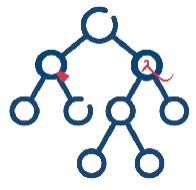
\includegraphics[height=1.0cm]{msca_logo.png}}%
    \end{center}

    \vspace{0.6cm}

    % Main title with Q logos on sides (with clickable links)
    \begin{center}
        \begin{minipage}{0.1\textwidth}
            \centering
            \href{https://quantlet.com}{
\includegraphics[height=1.1cm]{ql_logo.png}}
        \end{minipage}%
        \begin{minipage}{0.78\textwidth}
            \centering
            {\LARGE\bfseries\usebeamercolor[fg]{title}\inserttitle}

            \vspace{0.3cm}

            {\usebeamerfont{subtitle}\usebeamercolor[fg]{title}\insertsubtitle}
        \end{minipage}%
        \begin{minipage}{0.1\textwidth}
            \centering
            \href{https://quantinar.com}{
\includegraphics[height=1.1cm]{qr_logo.png}}
        \end{minipage}
    \end{center}

    \vspace{0.6cm}

    % Authors (left aligned)
    \hspace{0.5cm}{\usebeamerfont{author}\insertauthor}

    \vspace{0.3cm}

    % Institute/Affiliations (left aligned)
    \hspace{0.5cm}\begin{minipage}[t]{0.9\textwidth}
        \raggedright\small\insertinstitute
    \end{minipage}
}

%=============================================================================
% THEOREM ENVIRONMENTS
%=============================================================================
\theoremstyle{definition}
\setbeamertemplate{theorems}[numbered]
\ifdefined\atslang
\newtheorem{defn}{Definiție}
\newtheorem{thm}{Teoremă}
\newtheorem{prop}{Propoziție}
\newtheorem{rmk}{Observație}
\else
\newtheorem{defn}{Definition}
\newtheorem{thm}{Theorem}
\newtheorem{prop}{Proposition}
\newtheorem{rmk}{Remark}
\fi

%=============================================================================
% CENTRED MINIPAGE (no extra vertical space)
%=============================================================================
\newenvironment{cminipage}[1]{%
    \par\noindent\hfill\begin{minipage}{#1}\ignorespaces
}{%
    \end{minipage}\hfill\null\par
}

%=============================================================================
% CUSTOM COMMANDS
%=============================================================================
\newcommand{\E}{\mathbb{E}}
\newcommand{\Var}{\text{Var}}
\newcommand{\Cov}{\text{Cov}}
\newcommand{\Corr}{\text{Corr}}
\newcommand{\R}{\mathbb{R}}
\newcommand{\N}{\mathbb{N}}
\newcommand{\Z}{\mathbb{Z}}
\newcommand{\B}{\mathbf{B}}
\newcommand{\imark}{\textcolor{MainBlue}{\textbullet}}
\newcommand{\RMSE}{\text{RMSE}}
\newcommand{\MAE}{\text{MAE}}
\newcommand{\MAPE}{\text{MAPE}}

% Boldface vector/matrix commands (VAR, VECM, state space)
\newcommand{\bY}{\mathbf{Y}}
\newcommand{\bX}{\mathbf{X}}
\newcommand{\bA}{\mathbf{A}}
\newcommand{\bB}{\mathbf{B}}
\newcommand{\bepsilon}{\boldsymbol{\varepsilon}}
\newcommand{\bSigma}{\boldsymbol{\Sigma}}
\newcommand{\bPhi}{\boldsymbol{\Phi}}
\newcommand{\bGamma}{\boldsymbol{\Gamma}}
\newcommand{\bPi}{\boldsymbol{\Pi}}
\newcommand{\bc}{\mathbf{c}}
\newcommand{\balpha}{\boldsymbol{\alpha}}
\newcommand{\bbeta}{\boldsymbol{\beta}}
\newcommand{\bvarepsilon}{\boldsymbol{\varepsilon}}

% Seminar marks
\newcommand{\correct}{\textcolor{Forest}{\checkmark}}
\newcommand{\incorrect}{\textcolor{Crimson}{\texttimes}}
 se definește
%   \newcommand{\coursename}{Advanced Time Series Analysis and Forecasting}          (EN)
%   \newcommand{\coursename}{Analiza avansată a seriilor de timp și previziune}       (RO)  și  \def\atslang{ro}
% Fișierele .tex se află în EN/Courses, EN/Seminars, RO/Cursuri, RO/Seminarii (două niveluri sub rădăcină).
% Deck-urile sînt generate de latex/build_chapterN.py / build_seminarN.py (vezi latex/ats_build.py).

\documentclass[9pt, aspectratio=169, t]{beamer}
\providecommand{\coursename}{Advanced Time Series Analysis and Forecasting}

% Ensure content fits on slides
\setbeamersize{text margin left=8mm, text margin right=8mm}
% Smaller institute font (title page)
\setbeamerfont{institute}{size=\footnotesize}

%=============================================================================
% THEME AND STYLE CONFIGURATION
%=============================================================================
\usetheme{default}
% Using default theme for clean header/footer control

% Color Palette (matching Redispatch PDF)
\definecolor{MainBlue}{RGB}{26, 58, 110}
\definecolor{AccentBlue}{RGB}{26, 58, 110}
\definecolor{IDAred}{RGB}{205, 0, 0}
\definecolor{DarkGray}{RGB}{51, 51, 51}
\definecolor{MediumGray}{RGB}{128, 128, 128}
\definecolor{LightGray}{RGB}{248, 248, 248}
\definecolor{VeryLightGray}{RGB}{235, 235, 235}
\definecolor{KeynoteGray}{RGB}{218, 218, 218}
\definecolor{SectionGray}{RGB}{120, 120, 120}
\definecolor{FooterGray}{RGB}{100, 100, 100}
\definecolor{Crimson}{RGB}{220, 53, 69}
\definecolor{Forest}{RGB}{46, 125, 50}
\definecolor{Amber}{RGB}{181, 133, 63}
\definecolor{Orange}{RGB}{230, 126, 34}
\definecolor{Purple}{RGB}{142, 68, 173}

% Gradient background (exact Keynote 315° gradient: white to RGB 218,218,218)
\setbeamertemplate{background}{%
    \begin{tikzpicture}[remember picture, overlay]
        \shade[shading=axis, shading angle=315,
        top color=white, bottom color=KeynoteGray]
        (current page.south west) rectangle (current page.north east);
    \end{tikzpicture}%
}
% Fallback solid color for compatibility
\setbeamercolor{background canvas}{bg=}

\setbeamercolor{palette primary}{bg=MainBlue, fg=white}
\setbeamercolor{palette secondary}{bg=MainBlue!85, fg=white}
\setbeamercolor{palette tertiary}{bg=MainBlue!70, fg=white}
\setbeamercolor{structure}{fg=MainBlue}
\setbeamercolor{title}{fg=IDAred}
\setbeamercolor{frametitle}{fg=IDAred, bg=}
\setbeamercolor{block title}{bg=MainBlue, fg=white}
\setbeamercolor{block body}{bg=VeryLightGray, fg=DarkGray}
\setbeamercolor{block title alerted}{bg=Crimson, fg=white}
\setbeamercolor{block body alerted}{bg=Crimson!8, fg=DarkGray}
\setbeamercolor{block title example}{bg=Forest, fg=white}
\setbeamercolor{block body example}{bg=Forest!8, fg=DarkGray}
\setbeamercolor{item}{fg=MainBlue}

% Footer colors (override Madrid theme blue)
\setbeamercolor{author in head/foot}{fg=FooterGray, bg=}
\setbeamercolor{title in head/foot}{fg=FooterGray, bg=}
\setbeamercolor{date in head/foot}{fg=FooterGray, bg=}
\setbeamercolor{section in head/foot}{fg=FooterGray, bg=}
\setbeamercolor{subsection in head/foot}{fg=FooterGray, bg=}

% Bullet styles (apply everywhere including blocks)
\setbeamertemplate{itemize item}{\color{MainBlue}$\boxdot$}
\setbeamertemplate{itemize subitem}{\color{MainBlue}$\blacktriangleright$}
\setbeamertemplate{itemize subsubitem}{\color{MainBlue}\tiny$\bullet$}
\setbeamertemplate{itemize/enumerate body begin}{\normalsize}
\setbeamertemplate{itemize/enumerate subbody begin}{\normalsize}

% Item spacing - compact style
\setlength{\leftmargini}{10pt}       % Level 1: minimal indent
\setlength{\leftmarginii}{10pt}      % Level 2: minimal additional indent
% Compact list spacing (zero extra space before/after lists in blocks)
\makeatletter
\def\@listi{\leftmargin\leftmargini \topsep 0pt \parsep 0pt \itemsep 0pt}
\def\@listii{\leftmargin\leftmarginii \topsep 0pt \parsep 0pt \itemsep 0pt}
\makeatother

\setbeamertemplate{navigation symbols}{}

%=============================================================================
% CUSTOM HEADLINE
%=============================================================================
\setbeamertemplate{headline}{%
    \vskip10pt%
    \hbox to \paperwidth{%
        \hskip0.5cm%
        {\small\color{FooterGray}\renewcommand{\hyperlink}[2]{##2}\insertsectionhead}%
        \hfill%
        \textcolor{FooterGray}{\small\insertframenumber}%
        \hskip0.5cm%
    }%
    \vskip4pt%
    {\color{FooterGray}\hrule height 0.4pt}%
}

%=============================================================================
% CUSTOM FOOTER
%=============================================================================
\usepackage{fontawesome5}

\setbeamertemplate{footline}{%
    {\color{FooterGray}\hrule height 0.4pt}%
    \vskip4pt%
    \hbox to \paperwidth{%
        \hskip0.5cm%
        \textcolor{FooterGray}{\small\coursename}%
        \hfill%
        \raisebox{-0.1em}{%
            \begin{tikzpicture}[x=0.08em, y=0.08em, line width=0.4pt]
                \draw[FooterGray] (0,3) -- (1,4) -- (2,3.5) -- (3,5) -- (4,4) -- (5,6) -- (6,5.5) -- (7,4) -- (8,5) -- (9,7) -- (10,6) -- (11,5) -- (12,6.5) -- (13,8) -- (14,7) -- (15,6) -- (16,7.5) -- (17,9) -- (18,8) -- (19,7) -- (20,8.5) -- (21,10) -- (22,9) -- (23,8) -- (24,9.5);
            \end{tikzpicture}%
        }%
        \hskip0.5cm%
    }%
    \vskip6pt%
}

%=============================================================================
% PACKAGES
%=============================================================================
\usepackage[utf8]{inputenc}
\DeclareUnicodeCharacter{03B1}{\ensuremath{\alpha}}
\usepackage[T1]{fontenc}
\usepackage{amsmath, amssymb, amsthm}
\usepackage{mathtools}
\usepackage{bm}
\usepackage{tikz}
\usetikzlibrary{arrows.meta, positioning, shapes, calc, decorations.pathreplacing, shadings}
\usepackage{booktabs}
\usepackage{multirow}
\usepackage{array}
\usepackage{graphicx}
\usepackage{animate}
\usepackage{hyperref}
\usepackage{colortbl}
\usepackage{listings}
\lstset{language=Python, basicstyle=\ttfamily\scriptsize, keywordstyle=\color{MainBlue}\bfseries,
  commentstyle=\color{Forest}, stringstyle=\color{Crimson}, breaklines=true,
  frame=none, backgroundcolor=\color{VeryLightGray}, xleftmargin=2mm}
\hypersetup{colorlinks=true, linkcolor=MainBlue, urlcolor=MainBlue}
\graphicspath{{../../logos/}{../../charts/}{../../photos/}}
\usepackage{xcolor}
\hfuzz=2pt  % Suppress tiny overfull warnings (<2pt)
\vfuzz=2pt  % Suppress tiny vertical overfull warnings (<2pt)

%=============================================================================
% QUANTLET COMMANDS
%   \quantlet{<displayed name>}{<url>}       (generic)
%   \atsquantlet{Ch_05}{ATS_ch5_garch}       -> https://github.com/danpele/Advanced-Time-Series/tree/main/Quantlets/Ch_05/ATS_ch5_garch
%   \qlurl{<folder>} is defined per chapter by the generator (Quantlets/Ch_NN/<folder>)
%=============================================================================
\newcommand{\atsrepo}{https://github.com/danpele/Advanced-Time-Series}
\newcommand{\atsqlbase}{https://github.com/danpele/Advanced-Time-Series/tree/main/Quantlets}
\newcommand{\quantlet}[2]{%
    \hfill\href{#2}{%
        \raisebox{-0.15em}{
\includegraphics[height=0.7em]{ql_logo.png}}%
        \textcolor{MainBlue}{\tiny\ #1}%
    }%
}
\newcommand{\atsquantlet}[2]{\quantlet{\detokenize{#2}}{\atsqlbase/#1/#2}}

%=============================================================================
% NOTEBOOKS (Google Colab)
%   \colaburl{notebooks/EN/chapter5_seminar_notebook.ipynb} -> the Colab link of a file in the ATS repo
%   \nb: the chapter notebook (each seminar deck redefines it with \renewcommand)
%=============================================================================
\newcommand{\colaburl}[1]{https://colab.research.google.com/github/danpele/Advanced-Time-Series/blob/main/#1}
\newcommand{\nb}{https://colab.research.google.com/github/danpele/Advanced-Time-Series/tree/main/notebooks/EN}
\newcommand{\nbname}{notebooks/EN}

%=============================================================================
% SLIDE HELPERS (used by the generators; the same as in MFM)
%=============================================================================
% local font size for list bodies (the preamble forces \normalsize)
\newcommand{\itemsize}[1]{\setbeamertemplate{itemize/enumerate body begin}{#1}\setbeamertemplate{itemize/enumerate subbody begin}{#1}}
\newcommand{\intitle}[1]{{\hypersetup{urlcolor=white}#1}}   % white links inside coloured title bars
\newcommand{\imgcap}[1]{{\scriptsize #1}\\[0.5mm]}          % caption under a photo
\newcommand{\imgcredit}[2]{{\tiny\color{FooterGray}\href{#1}{#2}}}   % image credit: source URL, author/licence
\newcommand{\aiprompt}[1]{{\ttfamily\color{MainBlue}#1}}     % a prompt to an AI assistant

%=============================================================================
% SEMINARS: student version by default; the instructor wrapper *_solutions.tex sets \solutionstrue
%=============================================================================
\makeatletter\@ifundefined{ifsolutions}{\expandafter\newif\csname ifsolutions\endcsname}{}\makeatother
\newcommand{\solonly}[1]{\ifsolutions #1\fi}
\newcommand{\propsub}{\ifsolutions\else\framesubtitle{\ifdefined\atslang Rezolvarea se discută la seminar\else Solution discussed in class\fi}\fi}

%=============================================================================
% APPENDIX AND CHAPTER LINKS (latex/appendix_links.py writes the calls; it also re-declares these
% macros before \begin{document}, so the decks compile with or without this preamble block)
%=============================================================================
\providecommand{\atsapplink}[3]{\hypertarget{#2}{}\hyperlink{#1}{\beamergotobutton{#3}}}
\providecommand{\atsappback}[2]{\begin{tikzpicture}[remember picture,overlay]\node[anchor=south east] at ([xshift=-3mm,yshift=7mm]current page.south east){\hyperlink{#1}{\beamerreturnbutton{#2}}};\end{tikzpicture}}
\providecommand{\atschlink}[2]{\href{#1}{#2}}
\providecommand{\atschlinkt}[2]{\href{#1}{\usebeamercolor[fg]{frametitle}#2}}

%=============================================================================
% QUANTINAR COMMAND: link către un curs Quantinar (subiecte avansate)
%=============================================================================
\newcommand{\quantinar}[2]{%
    \href{#2}{%
        \raisebox{-0.15em}{
\includegraphics[height=0.8em]{qr_logo.png}}%
        \textcolor{MainBlue}{\scriptsize\ #1}%
    }%
}

%=============================================================================
% CUSTOM TITLE PAGE
%=============================================================================
\defbeamertemplate*{title page}{hybrid}[1][]
{
    \vspace{0.2cm}
    % Logos row - top header (with clickable links)
    \begin{center}
        \href{https://www.ase.ro}{
\includegraphics[height=1.0cm]{ase_logo.png}}\hspace{0.3cm}%
        \href{https://theida.net}{
\includegraphics[height=1.0cm]{ida_logo.png}}\hspace{0.3cm}%
        \href{https://blockchain-research-center.com}{
\includegraphics[height=1.0cm]{brc_logo.png}}\hspace{0.3cm}%
        \href{https://www.ai4efin.ase.ro}{
\includegraphics[height=1.0cm]{ai4efin_logo.png}}\hspace{0.3cm}%
        \href{https://ipe.ro/new}{
\includegraphics[height=1.0cm]{acad_logo.png}}\hspace{0.3cm}%
        \href{https://www.digital-finance-msca.com}{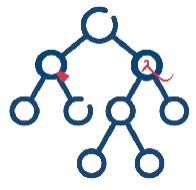
\includegraphics[height=1.0cm]{msca_logo.png}}%
    \end{center}

    \vspace{0.6cm}

    % Main title with Q logos on sides (with clickable links)
    \begin{center}
        \begin{minipage}{0.1\textwidth}
            \centering
            \href{https://quantlet.com}{
\includegraphics[height=1.1cm]{ql_logo.png}}
        \end{minipage}%
        \begin{minipage}{0.78\textwidth}
            \centering
            {\LARGE\bfseries\usebeamercolor[fg]{title}\inserttitle}

            \vspace{0.3cm}

            {\usebeamerfont{subtitle}\usebeamercolor[fg]{title}\insertsubtitle}
        \end{minipage}%
        \begin{minipage}{0.1\textwidth}
            \centering
            \href{https://quantinar.com}{
\includegraphics[height=1.1cm]{qr_logo.png}}
        \end{minipage}
    \end{center}

    \vspace{0.6cm}

    % Authors (left aligned)
    \hspace{0.5cm}{\usebeamerfont{author}\insertauthor}

    \vspace{0.3cm}

    % Institute/Affiliations (left aligned)
    \hspace{0.5cm}\begin{minipage}[t]{0.9\textwidth}
        \raggedright\small\insertinstitute
    \end{minipage}
}

%=============================================================================
% THEOREM ENVIRONMENTS
%=============================================================================
\theoremstyle{definition}
\setbeamertemplate{theorems}[numbered]
\ifdefined\atslang
\newtheorem{defn}{Definiție}
\newtheorem{thm}{Teoremă}
\newtheorem{prop}{Propoziție}
\newtheorem{rmk}{Observație}
\else
\newtheorem{defn}{Definition}
\newtheorem{thm}{Theorem}
\newtheorem{prop}{Proposition}
\newtheorem{rmk}{Remark}
\fi

%=============================================================================
% CENTRED MINIPAGE (no extra vertical space)
%=============================================================================
\newenvironment{cminipage}[1]{%
    \par\noindent\hfill\begin{minipage}{#1}\ignorespaces
}{%
    \end{minipage}\hfill\null\par
}

%=============================================================================
% CUSTOM COMMANDS
%=============================================================================
\newcommand{\E}{\mathbb{E}}
\newcommand{\Var}{\text{Var}}
\newcommand{\Cov}{\text{Cov}}
\newcommand{\Corr}{\text{Corr}}
\newcommand{\R}{\mathbb{R}}
\newcommand{\N}{\mathbb{N}}
\newcommand{\Z}{\mathbb{Z}}
\newcommand{\B}{\mathbf{B}}
\newcommand{\imark}{\textcolor{MainBlue}{\textbullet}}
\newcommand{\RMSE}{\text{RMSE}}
\newcommand{\MAE}{\text{MAE}}
\newcommand{\MAPE}{\text{MAPE}}

% Boldface vector/matrix commands (VAR, VECM, state space)
\newcommand{\bY}{\mathbf{Y}}
\newcommand{\bX}{\mathbf{X}}
\newcommand{\bA}{\mathbf{A}}
\newcommand{\bB}{\mathbf{B}}
\newcommand{\bepsilon}{\boldsymbol{\varepsilon}}
\newcommand{\bSigma}{\boldsymbol{\Sigma}}
\newcommand{\bPhi}{\boldsymbol{\Phi}}
\newcommand{\bGamma}{\boldsymbol{\Gamma}}
\newcommand{\bPi}{\boldsymbol{\Pi}}
\newcommand{\bc}{\mathbf{c}}
\newcommand{\balpha}{\boldsymbol{\alpha}}
\newcommand{\bbeta}{\boldsymbol{\beta}}
\newcommand{\bvarepsilon}{\boldsymbol{\varepsilon}}

% Seminar marks
\newcommand{\correct}{\textcolor{Forest}{\checkmark}}
\newcommand{\incorrect}{\textcolor{Crimson}{\texttimes}}
 se definește
%   \newcommand{\coursename}{Advanced Time Series Analysis and Forecasting}          (EN)
%   \newcommand{\coursename}{Analiza avansată a seriilor de timp și previziune}       (RO)  și  \def\atslang{ro}
% Fișierele .tex se află în EN/Courses, EN/Seminars, RO/Cursuri, RO/Seminarii (două niveluri sub rădăcină).
% Deck-urile sînt generate de latex/build_chapterN.py / build_seminarN.py (vezi latex/ats_build.py).

\documentclass[9pt, aspectratio=169, t]{beamer}
\providecommand{\coursename}{Advanced Time Series Analysis and Forecasting}

% Ensure content fits on slides
\setbeamersize{text margin left=8mm, text margin right=8mm}
% Smaller institute font (title page)
\setbeamerfont{institute}{size=\footnotesize}

%=============================================================================
% THEME AND STYLE CONFIGURATION
%=============================================================================
\usetheme{default}
% Using default theme for clean header/footer control

% Color Palette (matching Redispatch PDF)
\definecolor{MainBlue}{RGB}{26, 58, 110}
\definecolor{AccentBlue}{RGB}{26, 58, 110}
\definecolor{IDAred}{RGB}{205, 0, 0}
\definecolor{DarkGray}{RGB}{51, 51, 51}
\definecolor{MediumGray}{RGB}{128, 128, 128}
\definecolor{LightGray}{RGB}{248, 248, 248}
\definecolor{VeryLightGray}{RGB}{235, 235, 235}
\definecolor{KeynoteGray}{RGB}{218, 218, 218}
\definecolor{SectionGray}{RGB}{120, 120, 120}
\definecolor{FooterGray}{RGB}{100, 100, 100}
\definecolor{Crimson}{RGB}{220, 53, 69}
\definecolor{Forest}{RGB}{46, 125, 50}
\definecolor{Amber}{RGB}{181, 133, 63}
\definecolor{Orange}{RGB}{230, 126, 34}
\definecolor{Purple}{RGB}{142, 68, 173}

% Gradient background (exact Keynote 315° gradient: white to RGB 218,218,218)
\setbeamertemplate{background}{%
    \begin{tikzpicture}[remember picture, overlay]
        \shade[shading=axis, shading angle=315,
        top color=white, bottom color=KeynoteGray]
        (current page.south west) rectangle (current page.north east);
    \end{tikzpicture}%
}
% Fallback solid color for compatibility
\setbeamercolor{background canvas}{bg=}

\setbeamercolor{palette primary}{bg=MainBlue, fg=white}
\setbeamercolor{palette secondary}{bg=MainBlue!85, fg=white}
\setbeamercolor{palette tertiary}{bg=MainBlue!70, fg=white}
\setbeamercolor{structure}{fg=MainBlue}
\setbeamercolor{title}{fg=IDAred}
\setbeamercolor{frametitle}{fg=IDAred, bg=}
\setbeamercolor{block title}{bg=MainBlue, fg=white}
\setbeamercolor{block body}{bg=VeryLightGray, fg=DarkGray}
\setbeamercolor{block title alerted}{bg=Crimson, fg=white}
\setbeamercolor{block body alerted}{bg=Crimson!8, fg=DarkGray}
\setbeamercolor{block title example}{bg=Forest, fg=white}
\setbeamercolor{block body example}{bg=Forest!8, fg=DarkGray}
\setbeamercolor{item}{fg=MainBlue}

% Footer colors (override Madrid theme blue)
\setbeamercolor{author in head/foot}{fg=FooterGray, bg=}
\setbeamercolor{title in head/foot}{fg=FooterGray, bg=}
\setbeamercolor{date in head/foot}{fg=FooterGray, bg=}
\setbeamercolor{section in head/foot}{fg=FooterGray, bg=}
\setbeamercolor{subsection in head/foot}{fg=FooterGray, bg=}

% Bullet styles (apply everywhere including blocks)
\setbeamertemplate{itemize item}{\color{MainBlue}$\boxdot$}
\setbeamertemplate{itemize subitem}{\color{MainBlue}$\blacktriangleright$}
\setbeamertemplate{itemize subsubitem}{\color{MainBlue}\tiny$\bullet$}
\setbeamertemplate{itemize/enumerate body begin}{\normalsize}
\setbeamertemplate{itemize/enumerate subbody begin}{\normalsize}

% Item spacing - compact style
\setlength{\leftmargini}{10pt}       % Level 1: minimal indent
\setlength{\leftmarginii}{10pt}      % Level 2: minimal additional indent
% Compact list spacing (zero extra space before/after lists in blocks)
\makeatletter
\def\@listi{\leftmargin\leftmargini \topsep 0pt \parsep 0pt \itemsep 0pt}
\def\@listii{\leftmargin\leftmarginii \topsep 0pt \parsep 0pt \itemsep 0pt}
\makeatother

\setbeamertemplate{navigation symbols}{}

%=============================================================================
% CUSTOM HEADLINE
%=============================================================================
\setbeamertemplate{headline}{%
    \vskip10pt%
    \hbox to \paperwidth{%
        \hskip0.5cm%
        {\small\color{FooterGray}\renewcommand{\hyperlink}[2]{##2}\insertsectionhead}%
        \hfill%
        \textcolor{FooterGray}{\small\insertframenumber}%
        \hskip0.5cm%
    }%
    \vskip4pt%
    {\color{FooterGray}\hrule height 0.4pt}%
}

%=============================================================================
% CUSTOM FOOTER
%=============================================================================
\usepackage{fontawesome5}

\setbeamertemplate{footline}{%
    {\color{FooterGray}\hrule height 0.4pt}%
    \vskip4pt%
    \hbox to \paperwidth{%
        \hskip0.5cm%
        \textcolor{FooterGray}{\small\coursename}%
        \hfill%
        \raisebox{-0.1em}{%
            \begin{tikzpicture}[x=0.08em, y=0.08em, line width=0.4pt]
                \draw[FooterGray] (0,3) -- (1,4) -- (2,3.5) -- (3,5) -- (4,4) -- (5,6) -- (6,5.5) -- (7,4) -- (8,5) -- (9,7) -- (10,6) -- (11,5) -- (12,6.5) -- (13,8) -- (14,7) -- (15,6) -- (16,7.5) -- (17,9) -- (18,8) -- (19,7) -- (20,8.5) -- (21,10) -- (22,9) -- (23,8) -- (24,9.5);
            \end{tikzpicture}%
        }%
        \hskip0.5cm%
    }%
    \vskip6pt%
}

%=============================================================================
% PACKAGES
%=============================================================================
\usepackage[utf8]{inputenc}
\DeclareUnicodeCharacter{03B1}{\ensuremath{\alpha}}
\usepackage[T1]{fontenc}
\usepackage{amsmath, amssymb, amsthm}
\usepackage{mathtools}
\usepackage{bm}
\usepackage{tikz}
\usetikzlibrary{arrows.meta, positioning, shapes, calc, decorations.pathreplacing, shadings}
\usepackage{booktabs}
\usepackage{multirow}
\usepackage{array}
\usepackage{graphicx}
\usepackage{animate}
\usepackage{hyperref}
\usepackage{colortbl}
\usepackage{listings}
\lstset{language=Python, basicstyle=\ttfamily\scriptsize, keywordstyle=\color{MainBlue}\bfseries,
  commentstyle=\color{Forest}, stringstyle=\color{Crimson}, breaklines=true,
  frame=none, backgroundcolor=\color{VeryLightGray}, xleftmargin=2mm}
\hypersetup{colorlinks=true, linkcolor=MainBlue, urlcolor=MainBlue}
\graphicspath{{../../logos/}{../../charts/}{../../photos/}}
\usepackage{xcolor}
\hfuzz=2pt  % Suppress tiny overfull warnings (<2pt)
\vfuzz=2pt  % Suppress tiny vertical overfull warnings (<2pt)

%=============================================================================
% QUANTLET COMMANDS
%   \quantlet{<displayed name>}{<url>}       (generic)
%   \atsquantlet{Ch_05}{ATS_ch5_garch}       -> https://github.com/danpele/Advanced-Time-Series/tree/main/Quantlets/Ch_05/ATS_ch5_garch
%   \qlurl{<folder>} is defined per chapter by the generator (Quantlets/Ch_NN/<folder>)
%=============================================================================
\newcommand{\atsrepo}{https://github.com/danpele/Advanced-Time-Series}
\newcommand{\atsqlbase}{https://github.com/danpele/Advanced-Time-Series/tree/main/Quantlets}
\newcommand{\quantlet}[2]{%
    \hfill\href{#2}{%
        \raisebox{-0.15em}{
\includegraphics[height=0.7em]{ql_logo.png}}%
        \textcolor{MainBlue}{\tiny\ #1}%
    }%
}
\newcommand{\atsquantlet}[2]{\quantlet{\detokenize{#2}}{\atsqlbase/#1/#2}}

%=============================================================================
% NOTEBOOKS (Google Colab)
%   \colaburl{notebooks/EN/chapter5_seminar_notebook.ipynb} -> the Colab link of a file in the ATS repo
%   \nb: the chapter notebook (each seminar deck redefines it with \renewcommand)
%=============================================================================
\newcommand{\colaburl}[1]{https://colab.research.google.com/github/danpele/Advanced-Time-Series/blob/main/#1}
\newcommand{\nb}{https://colab.research.google.com/github/danpele/Advanced-Time-Series/tree/main/notebooks/EN}
\newcommand{\nbname}{notebooks/EN}

%=============================================================================
% SLIDE HELPERS (used by the generators; the same as in MFM)
%=============================================================================
% local font size for list bodies (the preamble forces \normalsize)
\newcommand{\itemsize}[1]{\setbeamertemplate{itemize/enumerate body begin}{#1}\setbeamertemplate{itemize/enumerate subbody begin}{#1}}
\newcommand{\intitle}[1]{{\hypersetup{urlcolor=white}#1}}   % white links inside coloured title bars
\newcommand{\imgcap}[1]{{\scriptsize #1}\\[0.5mm]}          % caption under a photo
\newcommand{\imgcredit}[2]{{\tiny\color{FooterGray}\href{#1}{#2}}}   % image credit: source URL, author/licence
\newcommand{\aiprompt}[1]{{\ttfamily\color{MainBlue}#1}}     % a prompt to an AI assistant

%=============================================================================
% SEMINARS: student version by default; the instructor wrapper *_solutions.tex sets \solutionstrue
%=============================================================================
\makeatletter\@ifundefined{ifsolutions}{\expandafter\newif\csname ifsolutions\endcsname}{}\makeatother
\newcommand{\solonly}[1]{\ifsolutions #1\fi}
\newcommand{\propsub}{\ifsolutions\else\framesubtitle{\ifdefined\atslang Rezolvarea se discută la seminar\else Solution discussed in class\fi}\fi}

%=============================================================================
% APPENDIX AND CHAPTER LINKS (latex/appendix_links.py writes the calls; it also re-declares these
% macros before \begin{document}, so the decks compile with or without this preamble block)
%=============================================================================
\providecommand{\atsapplink}[3]{\hypertarget{#2}{}\hyperlink{#1}{\beamergotobutton{#3}}}
\providecommand{\atsappback}[2]{\begin{tikzpicture}[remember picture,overlay]\node[anchor=south east] at ([xshift=-3mm,yshift=7mm]current page.south east){\hyperlink{#1}{\beamerreturnbutton{#2}}};\end{tikzpicture}}
\providecommand{\atschlink}[2]{\href{#1}{#2}}
\providecommand{\atschlinkt}[2]{\href{#1}{\usebeamercolor[fg]{frametitle}#2}}

%=============================================================================
% QUANTINAR COMMAND: link către un curs Quantinar (subiecte avansate)
%=============================================================================
\newcommand{\quantinar}[2]{%
    \href{#2}{%
        \raisebox{-0.15em}{
\includegraphics[height=0.8em]{qr_logo.png}}%
        \textcolor{MainBlue}{\scriptsize\ #1}%
    }%
}

%=============================================================================
% CUSTOM TITLE PAGE
%=============================================================================
\defbeamertemplate*{title page}{hybrid}[1][]
{
    \vspace{0.2cm}
    % Logos row - top header (with clickable links)
    \begin{center}
        \href{https://www.ase.ro}{
\includegraphics[height=1.0cm]{ase_logo.png}}\hspace{0.3cm}%
        \href{https://theida.net}{
\includegraphics[height=1.0cm]{ida_logo.png}}\hspace{0.3cm}%
        \href{https://blockchain-research-center.com}{
\includegraphics[height=1.0cm]{brc_logo.png}}\hspace{0.3cm}%
        \href{https://www.ai4efin.ase.ro}{
\includegraphics[height=1.0cm]{ai4efin_logo.png}}\hspace{0.3cm}%
        \href{https://ipe.ro/new}{
\includegraphics[height=1.0cm]{acad_logo.png}}\hspace{0.3cm}%
        \href{https://www.digital-finance-msca.com}{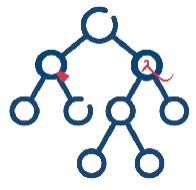
\includegraphics[height=1.0cm]{msca_logo.png}}%
    \end{center}

    \vspace{0.6cm}

    % Main title with Q logos on sides (with clickable links)
    \begin{center}
        \begin{minipage}{0.1\textwidth}
            \centering
            \href{https://quantlet.com}{
\includegraphics[height=1.1cm]{ql_logo.png}}
        \end{minipage}%
        \begin{minipage}{0.78\textwidth}
            \centering
            {\LARGE\bfseries\usebeamercolor[fg]{title}\inserttitle}

            \vspace{0.3cm}

            {\usebeamerfont{subtitle}\usebeamercolor[fg]{title}\insertsubtitle}
        \end{minipage}%
        \begin{minipage}{0.1\textwidth}
            \centering
            \href{https://quantinar.com}{
\includegraphics[height=1.1cm]{qr_logo.png}}
        \end{minipage}
    \end{center}

    \vspace{0.6cm}

    % Authors (left aligned)
    \hspace{0.5cm}{\usebeamerfont{author}\insertauthor}

    \vspace{0.3cm}

    % Institute/Affiliations (left aligned)
    \hspace{0.5cm}\begin{minipage}[t]{0.9\textwidth}
        \raggedright\small\insertinstitute
    \end{minipage}
}

%=============================================================================
% THEOREM ENVIRONMENTS
%=============================================================================
\theoremstyle{definition}
\setbeamertemplate{theorems}[numbered]
\ifdefined\atslang
\newtheorem{defn}{Definiție}
\newtheorem{thm}{Teoremă}
\newtheorem{prop}{Propoziție}
\newtheorem{rmk}{Observație}
\else
\newtheorem{defn}{Definition}
\newtheorem{thm}{Theorem}
\newtheorem{prop}{Proposition}
\newtheorem{rmk}{Remark}
\fi

%=============================================================================
% CENTRED MINIPAGE (no extra vertical space)
%=============================================================================
\newenvironment{cminipage}[1]{%
    \par\noindent\hfill\begin{minipage}{#1}\ignorespaces
}{%
    \end{minipage}\hfill\null\par
}

%=============================================================================
% CUSTOM COMMANDS
%=============================================================================
\newcommand{\E}{\mathbb{E}}
\newcommand{\Var}{\text{Var}}
\newcommand{\Cov}{\text{Cov}}
\newcommand{\Corr}{\text{Corr}}
\newcommand{\R}{\mathbb{R}}
\newcommand{\N}{\mathbb{N}}
\newcommand{\Z}{\mathbb{Z}}
\newcommand{\B}{\mathbf{B}}
\newcommand{\imark}{\textcolor{MainBlue}{\textbullet}}
\newcommand{\RMSE}{\text{RMSE}}
\newcommand{\MAE}{\text{MAE}}
\newcommand{\MAPE}{\text{MAPE}}

% Boldface vector/matrix commands (VAR, VECM, state space)
\newcommand{\bY}{\mathbf{Y}}
\newcommand{\bX}{\mathbf{X}}
\newcommand{\bA}{\mathbf{A}}
\newcommand{\bB}{\mathbf{B}}
\newcommand{\bepsilon}{\boldsymbol{\varepsilon}}
\newcommand{\bSigma}{\boldsymbol{\Sigma}}
\newcommand{\bPhi}{\boldsymbol{\Phi}}
\newcommand{\bGamma}{\boldsymbol{\Gamma}}
\newcommand{\bPi}{\boldsymbol{\Pi}}
\newcommand{\bc}{\mathbf{c}}
\newcommand{\balpha}{\boldsymbol{\alpha}}
\newcommand{\bbeta}{\boldsymbol{\beta}}
\newcommand{\bvarepsilon}{\boldsymbol{\varepsilon}}

% Seminar marks
\newcommand{\correct}{\textcolor{Forest}{\checkmark}}
\newcommand{\incorrect}{\textcolor{Crimson}{\texttimes}}


\newcommand{\qlurl}[1]{https://github.com/danpele/Advanced-Time-Series/tree/main/Quantlets/Ch_14/#1}

% Clickable citations (DOIs verified via Crossref)
\newcommand{\refAbG}{\href{https://doi.org/10.1257/000282803321455188}{Abadie and Gardeazabal (2003)}}
\newcommand{\refADHa}{\href{https://doi.org/10.1198/jasa.2009.ap08746}{Abadie, Diamond and Hainmueller (2010)}}
\newcommand{\refADHs}{\href{https://doi.org/10.18637/jss.v042.i13}{Abadie, Diamond and Hainmueller (2011)}}
\newcommand{\refADHb}{\href{https://doi.org/10.1111/ajps.12116}{Abadie, Diamond and Hainmueller (2015)}}
\newcommand{\refAba}{\href{https://doi.org/10.1257/jel.20191450}{Abadie (2021)}}
\newcommand{\refAJK}{\href{https://doi.org/10.1080/07350015.2016.1204919}{Angrist, Jordà and Kuersteiner (2018)}}
\newcommand{\refSDID}{\href{https://doi.org/10.1257/aer.20190159}{Arkhangelsky et al.\ (2021)}}
\newcommand{\refAI}{\href{https://doi.org/10.1257/jep.31.2.3}{Athey and Imbens (2017)}}
\newcommand{\refBBG}{\href{https://doi.org/10.1016/j.qref.2025.102006}{Babalos, Bouri and Gupta (2025)}}
\newcommand{\refBai}{\href{https://doi.org/10.3982/ECTA6135}{Bai (2009)}}
\newcommand{\refBBS}{\href{https://doi.org/10.1103/PhysRevLett.103.238701}{Barnett, Barrett and Seth (2009)}}
\newcommand{\refBaC}{\href{https://doi.org/10.1073/pnas.1700369114}{Baskerville and Cobey (2017)}}
\newcommand{\refASCM}{\href{https://doi.org/10.1080/01621459.2021.1929245}{Ben-Michael, Feller and Rothstein (2021)}}
\newcommand{\refBMKW}{\href{https://doi.org/10.1007/s10797-019-09566-5}{Benedek et al.\ (2020)}}
\newcommand{\refBoS}{\href{https://doi.org/10.1080/01621459.2018.1527225}{Bojinov and Shephard (2019)}}
\newcommand{\refBMSS}{\href{https://doi.org/10.1093/ej/uez020}{Born et al.\ (2019)}}
\newcommand{\refBrC}{\href{https://doi.org/10.1016/j.jeconom.2005.02.004}{Breitung and Candelon (2006)}}
\newcommand{\refCI}{\href{https://doi.org/10.1214/14-AOAS788}{Brodersen et al.\ (2015)}}
\newcommand{\refCSA}{\href{https://doi.org/10.1016/j.jeconom.2020.12.001}{Callaway and Sant’Anna (2021)}}
\newcommand{\refdCDH}{\href{https://doi.org/10.1257/aer.20181169}{de Chaisemartin and D’Haultfœuille (2020)}}
\newcommand{\refDML}{\href{https://doi.org/10.1111/ectj.12097}{Chernozhukov et al.\ (2018)}}
\newcommand{\refCWZ}{\href{https://doi.org/10.1080/01621459.2021.1920957}{Chernozhukov, Wüthrich and Zhu (2021)}}
\newcommand{\refDI}{\href{https://doi.org/10.3386/w22791}{Doudchenko and Imbens (2016)}}
\newcommand{\refDK}{\href{https://doi.org/10.1093/acprof:oso/9780199641178.001.0001}{Durbin and Koopman (2012)}}
\newcommand{\refEuroCT}{\href{https://ec.europa.eu/eurostat/databrowser/view/prc_hicp_ct/default/table}{Eurostat (2026b)}}
\newcommand{\refEuroM}{\href{https://ec.europa.eu/eurostat/web/hicp/methodology}{Eurostat (2026c)}}
\newcommand{\refFP}{\href{https://doi.org/10.3982/QE1596}{Ferman and Pinto (2021)}}
\newcommand{\refFiP}{\href{https://doi.org/10.1515/jci-2016-0026}{Firpo and Possebom (2018)}}
\newcommand{\refGew}{\href{https://doi.org/10.1080/01621459.1982.10477803}{Geweke (1982)}}
\newcommand{\refGB}{\href{https://doi.org/10.1016/j.jeconom.2021.03.014}{Goodman-Bacon (2021)}}
\newcommand{\refGra}{\href{https://doi.org/10.2307/1912791}{Granger (1969)}}
\newcommand{\refHam}{\href{https://doi.org/10.1515/9780691218632}{Hamilton (1994)}}
\newcommand{\refHar}{\href{https://doi.org/10.1017/CBO9781107049994}{Harvey (1989)}}
\newcommand{\refHCW}{\href{https://doi.org/10.1002/jae.1230}{Hsiao, Ching and Wan (2012)}}
\newcommand{\refIR}{\href{https://doi.org/10.1017/CBO9781139025751}{Imbens and Rubin (2015)}}
\newcommand{\refJor}{\href{https://doi.org/10.1257/0002828053828518}{Jordà (2005)}}
\newcommand{\refKL}{\href{https://doi.org/10.1017/9781108164818}{Kilian and Lütkepohl (2017)}}
\newcommand{\refLCG}{\href{https://doi.org/10.1093/ije/dyw098}{Lopez Bernal, Cummins and Gasparrini (2017)}}
\newcommand{\refMac}{\href{https://www.jstor.org/stable/2729691}{MacKinlay (1997)}}
\newcommand{\refMon}{\href{https://doi.org/10.1016/j.future.2016.12.009}{Mønster et al.\ (2017)}}
\newcommand{\refNW}{\href{https://doi.org/10.2307/1913610}{Newey and West (1987)}}
\newcommand{\refPea}{\href{https://doi.org/10.1017/CBO9780511803161}{Pearl (2009)}}
\newcommand{\refPMW}{\href{https://doi.org/10.3982/ECTA17813}{Plagborg-Møller and Wolf (2021)}}
\newcommand{\refRS}{\href{https://arxiv.org/abs/1903.01637}{Rambachan and Shephard (2021)}}
\newcommand{\refRSBP}{\href{https://doi.org/10.1016/j.jeconom.2023.03.008}{Roth et al.\ (2023)}}
\newcommand{\refRub}{\href{https://doi.org/10.1037/h0037350}{Rubin (1974)}}
\newcommand{\refPCMCI}{\href{https://doi.org/10.1126/sciadv.aau4996}{Runge et al.\ (2019a)}}
\newcommand{\refRunE}{\href{https://doi.org/10.1038/s41467-019-10105-3}{Runge et al.\ (2019b)}}
\newcommand{\refSch}{\href{https://doi.org/10.1103/PhysRevLett.85.461}{Schreiber (2000)}}
\newcommand{\refSV}{\href{https://doi.org/10.1504/IJMMNO.2014.059942}{Scott and Varian (2014)}}
\newcommand{\refSEC}{\href{https://www.sec.gov/files/rules/sro/nysearca/2024/34-99306.pdf}{SEC (2024)}}
\newcommand{\refSims}{\href{https://www.jstor.org/stable/1806097}{Sims (1972)}}
\newcommand{\refSGS}{\href{https://doi.org/10.7551/mitpress/1754.001.0001}{Spirtes, Glymour and Scheines (2000)}}
\newcommand{\refSW}{\href{https://doi.org/10.1111/ecoj.12593}{Stock and Watson (2018)}}
\newcommand{\refSug}{\href{https://doi.org/10.1126/science.1227079}{Sugihara et al.\ (2012)}}
\newcommand{\refSA}{\href{https://doi.org/10.1016/j.jeconom.2020.09.006}{Sun and Abraham (2021)}}
\newcommand{\refTY}{\href{https://doi.org/10.1016/0304-4076(94)01616-8}{Toda and Yamamoto (1995)}}
\newcommand{\refXu}{\href{https://doi.org/10.1017/pan.2016.2}{Xu (2017)}}
\newcommand{\refYDGS}{\href{https://doi.org/10.1038/srep14750}{Ye et al.\ (2015)}}
\newcommand{\refKPSb}{\href{https://doi.org/10.1186/s41937-017-0004-9}{Klößner et al.\ (2018)}}
\newcommand{\refFrP}{\href{https://doi.org/10.1103/PhysRevLett.99.204101}{Frenzel and Pompe (2007)}}
\newcommand{\refKSG}{\href{https://doi.org/10.1103/PhysRevE.69.066138}{Kraskov, Stögbauer and Grassberger (2004)}}
\newcommand{\refKKPS}{\href{https://doi.org/10.1080/07350015.2021.1930012}{Kaul et al.\ (2022)}}
\newcommand{\refAnd}{\href{https://doi.org/10.1111/1468-0262.00466}{Andrews (2003)}}
\newcommand{\refTak}{\href{https://doi.org/10.1007/BFb0091924}{Takens (1981)}}
\newcommand{\refADHd}{\href{https://doi.org/10.7910/DVN/24714}{Abadie, Diamond and Hainmueller (2014)}}
\newcommand{\refOECD}{\href{https://sdmx.oecd.org/public/rest/dataflow/OECD.SDD.NAD/DSD_NAMAIN1@DF_QNA/1.1}{OECD (2026)}}
\newcommand{\refEuroH}{\href{https://ec.europa.eu/eurostat/databrowser/view/prc_hicp_minr/default/table}{Eurostat (2026a)}}

\title[Advanced Time Series Analysis and Forecasting]{Advanced Time Series Analysis and Forecasting}
\subtitle{Chapter 14: Causal inference for time series}
\author[D.T. Pele]{Daniel Traian PELE}
\institute{Bucharest University of Economic Studies\\
IDA Institute Digital Assets\\
Blockchain Research Center\\
AI4EFin Artificial Intelligence for Energy Finance\\
Romanian Academy, Institute for Economic Forecasting\\
MSCA Digital Finance}
\date{}

%=============================================================================
\providecommand{\atsapplink}[3]{\hypertarget{#2}{}\hyperlink{#1}{\beamergotobutton{#3}}}  % APPLINKS-MACROS
\providecommand{\atsappback}[2]{\begin{tikzpicture}[remember picture,overlay]\node[anchor=south east] at ([xshift=-3mm,yshift=7mm]current page.south east){\hyperlink{#1}{\beamerreturnbutton{#2}}};\end{tikzpicture}}  % APPLINKS-MACROS
\providecommand{\atschlink}[2]{\href{#1}{#2}}  % APPLINKS-MACROS
\providecommand{\atschlinkt}[2]{\href{#1}{\usebeamercolor[fg]{frametitle}#2}}  % APPLINKS-MACROS
\begin{document}
%=============================================================================

{
\setbeamertemplate{headline}{}
\setbeamertemplate{footline}{}
\begin{frame}[noframenumbering]
    \titlepage
\end{frame}
}
% BEGIN-ACRONYMS (generat de latex/acronyms.py; nu editati manual)
\begin{frame}{Acronyms used in this material (1/2)}
\setbeamertemplate{itemize/enumerate body begin}{\footnotesize}
\begin{columns}[T]
\begin{column}{0.49\textwidth}
\begin{itemize}\setlength{\itemsep}{0pt}
    \item \textbf{ADH}: Abadie, Diamond and Hainmueller
    \item \textbf{AI}: Artificial Intelligence
    \item \textbf{AR}: AutoRegressive (model); in event studies: Abnormal Return
    \item \textbf{BET}: Bucharest Exchange Trading (index)
    \item \textbf{BNR}: Banca Națională a României (the National Bank of Romania)
    \item \textbf{BSTS}: Bayesian Structural Time Series
    \item \textbf{CAR}: Cumulative Abnormal Return
    \item \textbf{CCM}: Convergent Cross Mapping
    \item \textbf{CS}: Callaway and Sant'Anna (estimator)
    \item \textbf{DML}: Double/Debiased Machine Learning
\end{itemize}
\end{column}
\begin{column}{0.49\textwidth}
\begin{itemize}\setlength{\itemsep}{0pt}
    \item \textbf{ECOFIN}: Economic and Financial Affairs Council (of the EU)
    \item \textbf{EODHD}: EOD Historical Data (market-data provider)
    \item \textbf{EU}: European Union
    \item \textbf{EU-26}: the 26 EU countries other than Romania
    \item \textbf{GDP}: Gross Domestic Product
    \item \textbf{HAC}: Heteroskedasticity and Autocorrelation Consistent (standard errors)
    \item \textbf{HICP}: Harmonised Index of Consumer Prices
    \item \textbf{ITS}: Interrupted Time Series
    \item \textbf{LLM}: Large Language Model
\end{itemize}
\end{column}
\end{columns}
\end{frame}
\begin{frame}{Acronyms used in this material (2/2)}
\setbeamertemplate{itemize/enumerate body begin}{\footnotesize}
\begin{columns}[T]
\begin{column}{0.49\textwidth}
\begin{itemize}\setlength{\itemsep}{0pt}
    \item \textbf{LP}: Local Projection
    \item \textbf{MCI}: Momentary Conditional Independence
    \item \textbf{MCMC}: Markov Chain Monte Carlo
    \item \textbf{MSPE}: Mean Squared Prediction Error
    \item \textbf{OECD}: Organisation for Economic Co-operation and Development
    \item \textbf{OLS}: Ordinary Least Squares
    \item \textbf{PC1}: first Principal Component
    \item \textbf{PCMCI}: PC algorithm + Momentary Conditional Independence
    \item \textbf{RMSPE}: Root Mean Squared Prediction Error
    \item \textbf{SC}: Synthetic Control
\end{itemize}
\end{column}
\begin{column}{0.49\textwidth}
\begin{itemize}\setlength{\itemsep}{0pt}
    \item \textbf{SDID}: Synthetic Difference in Differences
    \item \textbf{SEC}: Securities and Exchange Commission
    \item \textbf{SVAR}: Structural Vector AutoRegression
    \item \textbf{TE}: Transfer Entropy
    \item \textbf{TWFE}: Two-Way Fixed Effects
    \item \textbf{UK}: United Kingdom
    \item \textbf{US}: United States
    \item \textbf{USA}: United States of America
    \item \textbf{VAR}: Vector AutoRegression
    \item \textbf{VAT}: Value Added Tax
    \item \textbf{VIX}: CBOE Volatility IndeX
\end{itemize}
\end{column}
\end{columns}
\end{frame}
% END-ACRONYMS

\begin{frame}{Today's question and route}
\itemsize{\small}
\begin{itemize}
    \item \textbf{Question}: when does a time-series analysis tell us what \textit{would have happened} without a shock or a policy, and how sure can we be?
    \begin{itemize}
        \item prediction is not intervention: a variable can forecast another without causing it
    \end{itemize}
    \item \textbf{Route} of the chapter
    \begin{itemize}
        \item Granger causality, potential outcomes for time series, transfer entropy
        \item causal discovery: PCMCI and convergent cross mapping, with their limits
        \item interrupted time series and event studies with dependent errors
        \item synthetic control and its successors; staggered DiD; CausalImpact; DML
    \end{itemize}
    \item We build on \atschlink{https://danpele.github.io/Advanced-Time-Series/EN/Courses/chapter0_refresher_inference.pdf}{Chapter 0} (HAC), \atschlink{https://danpele.github.io/Advanced-Time-Series/EN/Courses/chapter3_structural_var_local_projections.pdf}{Chapter 3} (SVAR, local projections, proxy SVAR) and \atschlink{https://danpele.github.io/Advanced-Time-Series/EN/Courses/chapter6_state_space_models_bayesian_filtering.pdf}{Chapter 6} (state space, BSTS); Seminar 14 comes before this lecture
\end{itemize}
\end{frame}

\begin{frame}{Learning outcomes}
\itemsize{\small}
\begin{itemize}
    \item Distinguish Granger causality from a dynamic causal effect, and state the conditions under which a time-series estimand has a causal meaning
    \item Run conditional Granger tests with HAC covariance, estimate transfer entropy, and read the output of PCMCI and convergent cross mapping critically
    \item Estimate interrupted-time-series and event-study effects with standard errors that respect serial dependence
    \item Build synthetic controls (classic, demeaned, augmented, synthetic DiD), run placebo inference, and replicate a published result
    \item Use CausalImpact-type state space counterfactuals and judge the identifying assumptions of every method honestly
\end{itemize}
\end{frame}

\begin{frame}{Reading, data and tools}
\itemsize{\small}
\begin{itemize}
    \item Causality and time series: \refGra; \refSims; \refRS; \refBoS; \refAJK; \refSW
    \begin{itemize}
        \item discovery: \refSch; \refPCMCI; \refRunE; \refSug
    \end{itemize}
    \item Policy evaluation
    \begin{itemize}
        \item synthetic control: \refADHa; \refADHb; \refAba; \refASCM; \refSDID
        \item staggered DiD and CausalImpact: \refCSA; \refCI; survey \refAI
    \end{itemize}
    \item Python Quantlets of this chapter: \href{https://github.com/danpele/Advanced-Time-Series/tree/main/Quantlets/Ch_14}{Quantlets/Ch\_14}
    \begin{itemize}
        \item \texttt{numpy}, \texttt{scipy} (synthetic control weights by quadratic programming) and \texttt{statsmodels} (state space); every estimator written out, no black box
    \end{itemize}
    \item Lecture notebook: \href{\colaburl{notebooks/EN/chapter14_lecture_notebook.ipynb}}{open in Google Colab}
\end{itemize}
\end{frame}

\begin{frame}{Data used in this chapter}
\itemsize{\footnotesize}
\begin{center}
\scriptsize
\begin{tabular}{>{\raggedright\arraybackslash}p{3.3cm}>{\raggedright\arraybackslash}p{5.6cm}>{\raggedright\arraybackslash}p{3.4cm}}
\toprule
\textbf{Series} & \textbf{Source, sample} & \textbf{Use} \\
\midrule
HICP inflation, 27 EU countries; HICP at constant tax rates & \refEuroH, \refEuroCT: monthly, 2015 -- August 2026 & ITS, synthetic control for Romania \\
GDP per capita, West Germany and 16 OECD countries & \refADHd: 1960--2003 & replication of ADH (2015) \\
Real GDP, UK and 23 OECD countries & \refOECD: quarterly, 1995--2019 & Brexit doppelganger \\
Daily index and crypto prices; EUR/RON & EODHD; BNR reference rate; to 18 September 2026 & Granger, PCMCI, event study, CausalImpact \\
\bottomrule
\end{tabular}
\end{center}
\begin{itemize}
    \item Treatment dates, sample windows and estimators are fixed before the post-treatment data are looked at; every placebo is reported
\end{itemize}
\end{frame}

\begin{frame}{Two languages of causality}
\itemsize{\small}
\begin{columns}[T]
\begin{column}{0.36\textwidth}
\centering

\includegraphics[height=0.28\textheight]{ch14_pearl_2013.jpg}\\[1mm]
\imgcap{Judea Pearl, Turing Award 2011}
\imgcredit{https://commons.wikimedia.org/wiki/File:Judea_Pearl_at_NIPS_2013_(11781981594)_(cropped).jpg}{Photo: Better Than Bacon (2013); CC BY 2.0; Wikimedia Commons}\\[1mm]\centering
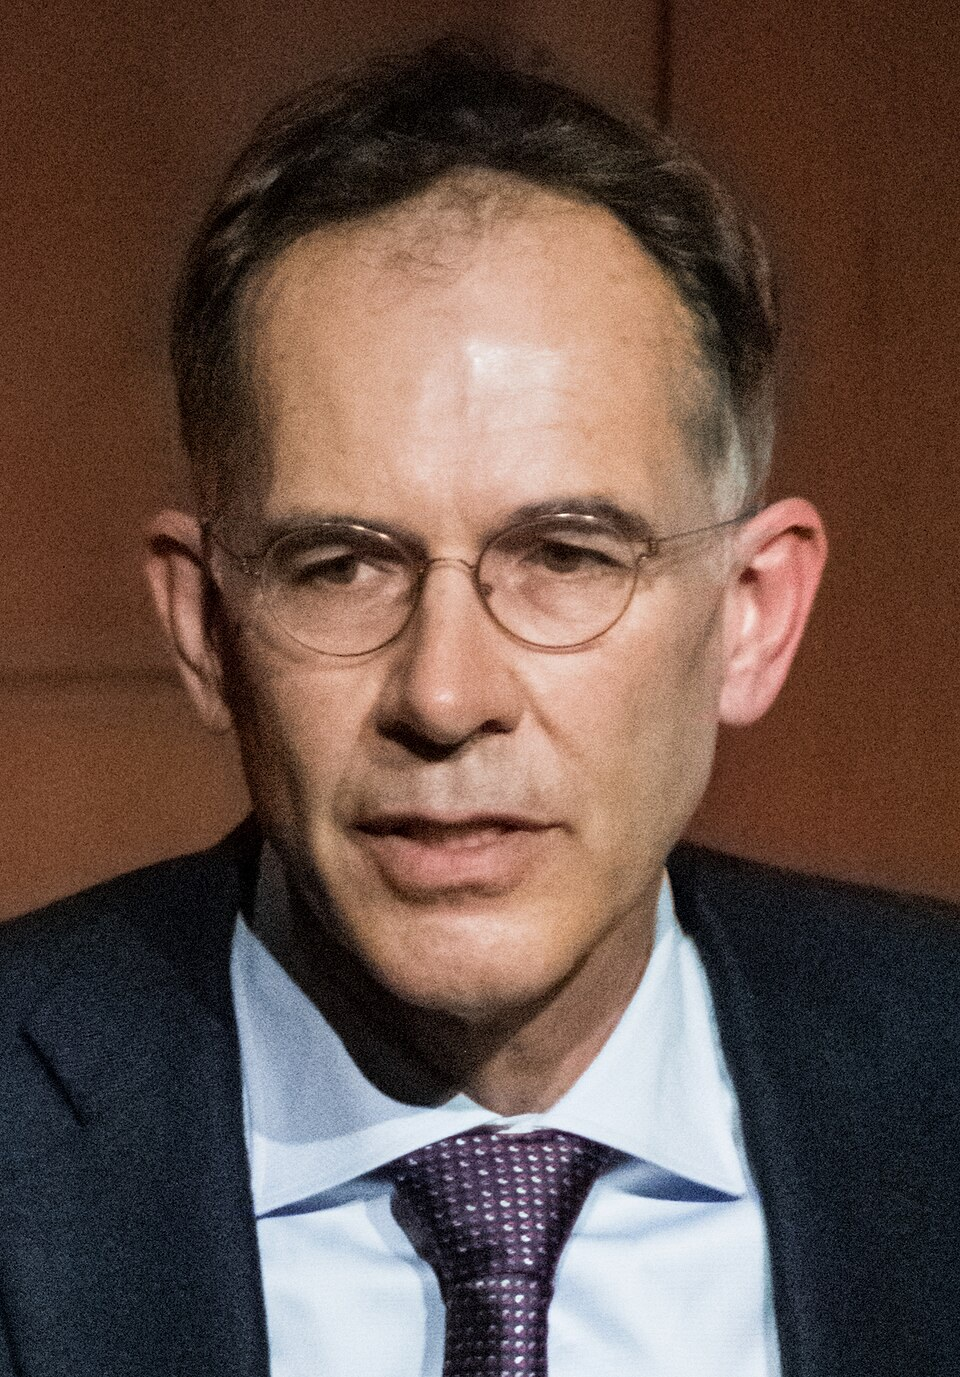
\includegraphics[height=0.20\textheight]{ch14_imbens_2022.jpg}\\[1mm]
\imgcap{Guido Imbens, Nobel Prize in Economics 2021}
\imgcredit{https://commons.wikimedia.org/wiki/File:Guido_Imbens_Lemley_Lecture_1_(cropped).jpg}{Photo: Filetime (2022); CC0; Wikimedia Commons}
\end{column}
\begin{column}{0.62\textwidth}
\begin{itemize}
    \item \textbf{Structural causal models} \refPea
    \begin{itemize}
        \item graphs and the $do(\cdot)$ operator: $do(X = x)$ sets $X$ by intervention instead of observing it
        \item conditions under which a causal effect is identified from observational data
    \end{itemize}
    \item \textbf{Potential outcomes} \refRub, \refIR
    \begin{itemize}
        \item $Y(1)$, $Y(0)$: the outcomes of one unit with and without treatment; only one of them is observed
        \item assignment mechanisms; design before analysis
    \end{itemize}
    \item \textbf{Time series} add order, dependence and a single realisation
    \begin{itemize}
        \item one country, one history, one treatment path
        \item Granger and PCMCI speak the graph language; synthetic control, DiD and CausalImpact speak potential outcomes
    \end{itemize}
\end{itemize}
\end{column}
\end{columns}
\end{frame}

\begin{frame}{Four case studies}
\itemsize{\footnotesize}
\begin{center}
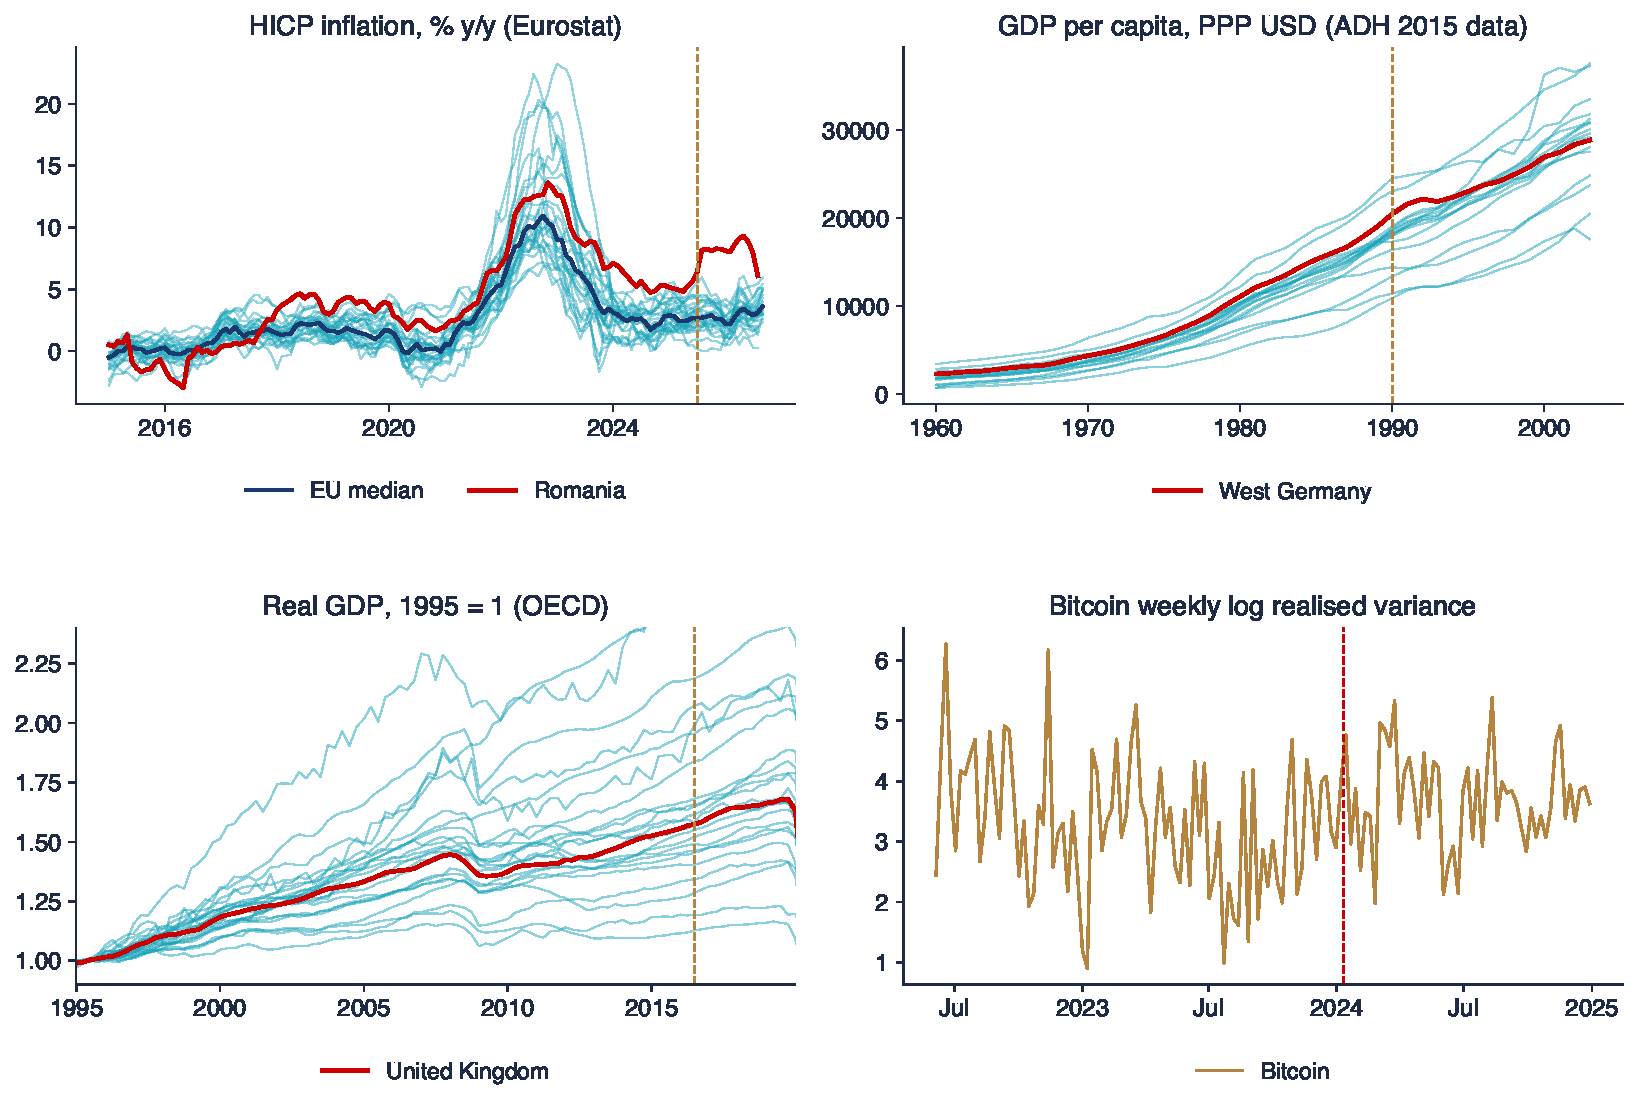
\includegraphics[width=0.97\textwidth,height=0.58\textheight,keepaspectratio]{ats_ch14_overview.pdf}
\end{center}
\vspace{-0.25cm}
\begin{itemize}
    \item Romanian inflation against 26 EU countries; West Germany against the OECD sample; UK real GDP against 23 OECD countries; Bitcoin realised variance around the spot ETF approval
\end{itemize}
\quantlet{ATS\_ch14\_romania}{\qlurl{ATS_ch14_romania}}
\end{frame}

\begin{frame}{Interpreting the four case studies}
\itemsize{\small}
\begin{itemize}
    \item Romania: annual HICP inflation 5.6\% in June 2025, 8.2\% in August 2025, peak 9.3\% in May 2026; 6.1\% in August 2026 (EU median 3.1\%)
    \item Each case has one treated unit and a pool of untreated units or controls observed over a long pre-period: the comparative-case-study design
    \item Romania is outside the range of the donors before the treatment (the highest inflation in the EU): a warning for every method that interpolates
    \item Bitcoin volatility is noisy and the controls are weak: the setting where an honest analysis may find nothing
\end{itemize}
\end{frame}


%=============================================================================
\section{Granger causality and causal effects}
%=============================================================================

\begin{frame}{Known from TSA and \atschlinkt{https://danpele.github.io/Advanced-Time-Series/EN/Courses/chapter3_structural_var_local_projections.pdf}{Chapter 3}, and new here}
\itemsize{\small}
\begin{itemize}
    \item Known: the bivariate Granger test in a VAR (\atschlink{https://danpele.github.io/Time-Series-Analysis/EN/Courses/chapter6_var_models_granger_causality.pdf}{TSA, Chapter 6}); SVAR identification, local projections and proxy SVAR (\atschlink{https://danpele.github.io/Advanced-Time-Series/EN/Courses/chapter3_structural_var_local_projections.pdf}{Chapter 3}); HAC (\atschlink{https://danpele.github.io/Advanced-Time-Series/EN/Courses/chapter0_refresher_inference.pdf}{Chapter 0}); Kalman filter and BSTS (\atschlink{https://danpele.github.io/Advanced-Time-Series/EN/Courses/chapter6_state_space_models_bayesian_filtering.pdf}{Chapter 6})
    \item New: what these tools can and cannot say about interventions
    \begin{itemize}
        \item potential outcomes for time series; non-anticipation; when an impulse response is a causal effect
        \item nonlinear and graph-based discovery; comparative case studies with one treated unit
    \end{itemize}
    \item Replications: Abadie, Diamond and Hainmueller (2015, Table 1, Figures 2--5); Born et al.\ (2019, Table 2, Figure 2); Sugihara et al.\ (2012, Figure 3)
\end{itemize}
\end{frame}

\begin{frame}{Granger causality: the definition (1/2)}
\itemsize{\small}
\begin{itemize}
    \item \refGra: $x$ \textbf{Granger-causes} $y$ if the past of $x$ lowers the mean squared error of the best one-step forecast of $y$ \[ \E\big[(y_{t+1} - \E[y_{t+1}\mid \mathcal I_t])^2\big] < \E\big[(y_{t+1} - \E[y_{t+1}\mid \mathcal I_t\setminus x])^2\big] \]
    \begin{itemize}
        \item $\mathcal I_t$: all the information available up to $t$; $\mathcal I_t\setminus x$: the same information without the past of $x$
        \item $\E[y_{t+1}\mid\cdot]$: the conditional mean, i.e.\ the best forecast in mean squared error
    \end{itemize}
    \item In practice $\mathcal I_t$ is a finite set of lags in a regression \[ y_t = c + \sum_{j=1}^p a_jy_{t-j} + \sum_{j=1}^p b_jx_{t-j} + \sum_{j=1}^p \gamma_j'z_{t-j} + u_t \]
    \begin{itemize}
        \item $p$: the number of lags; $a_j$, $b_j$: coefficients on the lags of $y$ and of $x$; $z_t$: a vector of other conditioning series, with coefficient vectors $\gamma_j$; $u_t$: the error
        \item null hypothesis of Granger non-causality: $H_0$: $b_1 = \dots = b_p = 0$
    \end{itemize}
\end{itemize}
\end{frame}

\begin{frame}{Granger causality: the definition (2/2)}
\itemsize{\small}
\begin{itemize}
    \item \textbf{Wald statistic}: a quadratic form of the estimated lag coefficients of $x$ \[ W = \hat b'\hat V_b^{-1}\hat b \;\to\; \chi^2_p \quad \text{under} \ H_0 \]
    \begin{itemize}
        \item $\hat b = (\hat b_1, \dots, \hat b_p)'$; $\hat V_b$: its estimated covariance matrix; reject $H_0$ for a large $W$ (small p-value)
        \item $\hat V_b$ HAC (\atschlink{https://danpele.github.io/Advanced-Time-Series/EN/Courses/chapter0_refresher_inference.pdf}{Chapter 0}) when $u_t$ is heteroskedastic, as for returns \refNW
    \end{itemize}
    \item Integrated or cointegrated series \refTY
    \begin{itemize}
        \item add as many extra lags as the maximal order of integration and test only the first $p$ lags
    \end{itemize}
    \item \textbf{Strength}: the Geweke measure \refGew, decomposable by frequency \refBrC{} (\atschlink{https://danpele.github.io/Advanced-Time-Series/EN/Courses/chapter11_spectral_wavelet_analysis.pdf}{Chapter 11}) \[ F_{x\to y} = \ln\big(\sigma^2_{\mathrm{restricted}}/\sigma^2_{\mathrm{full}}\big) \]
    \begin{itemize}
        \item $\sigma^2_{\mathrm{restricted}}$, $\sigma^2_{\mathrm{full}}$: residual variances of the regression without and with the lags of $x$; $F_{x\to y} \ge 0$, and 0 means no Granger causality
    \end{itemize}
\end{itemize}
\end{frame}

\begin{frame}{Granger causality is about prediction}
\itemsize{\small}
\begin{columns}[T]
\begin{column}{0.36\textwidth}
\centering
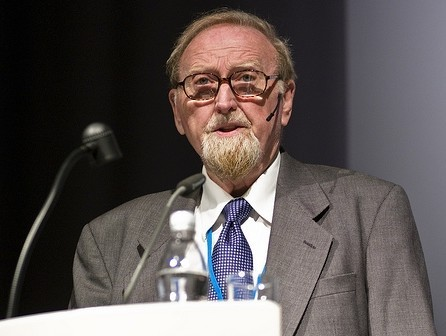
\includegraphics[height=0.44\textheight]{ch1_granger_2008.jpg}\\[1mm]
\imgcap{Clive Granger, Nobel Prize in Economics 2003}
\imgcredit{https://commons.wikimedia.org/wiki/File:Clive_Granger_by_Olaf_Storbeck.jpg}{Photo: Olaf Storbeck (2008); CC BY-SA 2.0; Wikimedia Commons}
\end{column}
\begin{column}{0.62\textwidth}
\begin{itemize}
    \item Four ways in which $x$ Granger-causes $y$ without causing it
    \begin{itemize}
        \item \textbf{common driver} $z$, omitted, reaching $x$ and $y$ at different lags
        \item \textbf{expectations}: asset prices move before the events they anticipate (stock prices ``cause'' GDP; \refSims)
        \item \textbf{timing}: different closing hours, aggregation and sampling turn instantaneous links into lagged ones
        \item \textbf{measurement error} in $y$ that $x$ helps to filter
    \end{itemize}
    \item And the reverse: a true effect can be invisible to the test
    \begin{itemize}
        \item nonlinear, contemporaneous, or offset by policy feedback
    \end{itemize}
\end{itemize}
\end{column}
\end{columns}
\end{frame}

\begin{frame}{A common driver creates Granger causality}
\itemsize{\footnotesize}
\begin{center}
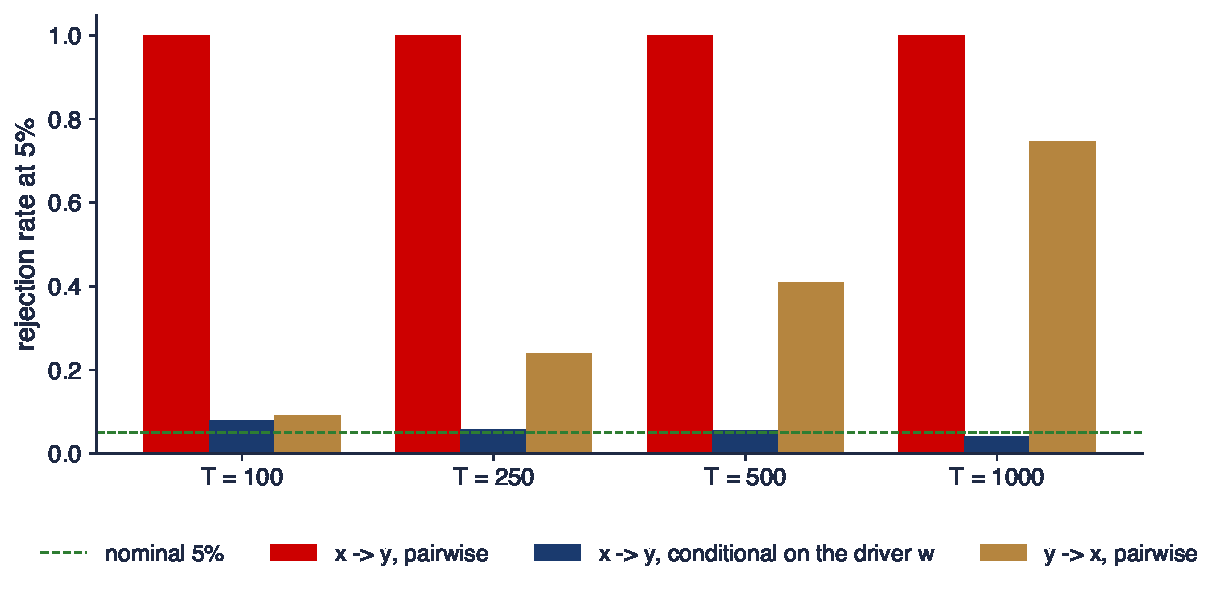
\includegraphics[width=0.97\textwidth,height=0.5\textheight,keepaspectratio]{ats_ch14_granger_sim.pdf}
\end{center}
\vspace{-0.25cm}
\begin{itemize}
    \item Simulated system: a driver $w_t = 0.9w_{t-1} + \eta_t$ (AR(1), $\phi = 0.9$); $x_t = w_{t-1} + e_t$, $y_t = w_{t-3} + u_t$; $\eta_t, e_t, u_t$: independent noise
    \item $x$ has no effect on $y$; tests with $p = 2$ lags (pairwise) and $p = 4$ (conditional on $w$), 500 replications
\end{itemize}
\quantlet{ATS\_ch14\_granger}{\qlurl{ATS_ch14_granger}}
\end{frame}

\begin{frame}{Interpreting the common-driver experiment}
\itemsize{\small}
\begin{itemize}
    \item Pairwise, $x$ ``Granger-causes'' $y$ in 100\% of the samples already at $T = 100$: $x$ carries news about $w$ two periods before $y$ does
    \item Conditional on the driver the rejection rate falls to the nominal level (4\% at $T = 1000$): Granger causality is relative to the information set
    \item The reverse test also rejects more and more (9\% at $T = 100$, 75\% at $T = 1000$): the past of $y$ is informative about the persistent driver as well
    \item Larger samples make a spurious finding more certain, not less: power is not validity
\end{itemize}
\end{frame}

\begin{frame}{Lead and lag between New York, Frankfurt and Bucharest}
\itemsize{\footnotesize}
\begin{center}
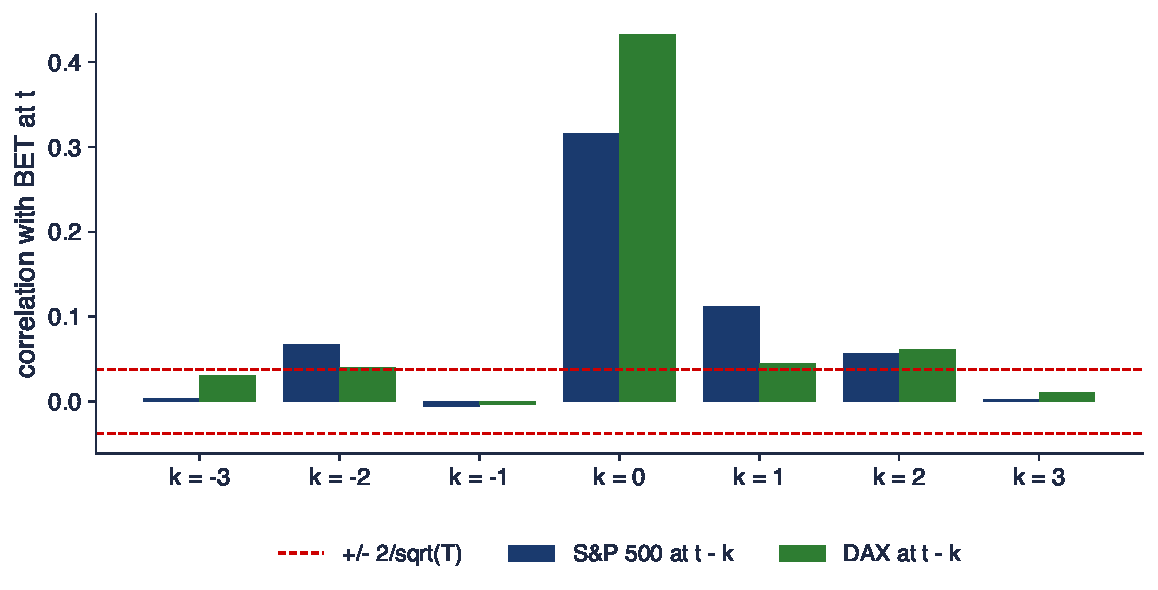
\includegraphics[width=0.97\textwidth,height=0.56\textheight,keepaspectratio]{ats_ch14_granger_markets.pdf}
\end{center}
\vspace{-0.25cm}
\begin{itemize}
    \item Daily log returns, common trading days 6 January 2015 -- 18 September 2026 ($T = 2\,815$); correlation of the BET at $t$ with the S\&P 500 and the DAX at $t - k$
\end{itemize}
\quantlet{ATS\_ch14\_granger}{\qlurl{ATS_ch14_granger}}
\end{frame}

\begin{frame}{Granger tests on the three indices}
\itemsize{\small}
\begin{center}
\footnotesize
\begin{tabular}{lccc}
\toprule
\textbf{Hypothesis} ($p = 2$) & \textbf{Wald (HAC)} & $p$\textbf{-value} & \textbf{conditioning} \\
\midrule
S\&P 500 $\not\to$ BET & 15.3 & $<$0.001 & -- \\
BET $\not\to$ S\&P 500 & 4.5 & 0.105 & -- \\
S\&P 500 $\not\to$ BET & 9.9 & 0.007 & DAX \\
DAX $\not\to$ BET & 1.6 & 0.449 & -- \\
S\&P 500 $\not\to$ DAX & 18.3 & $<$0.001 & -- \\
\bottomrule
\end{tabular}
\end{center}
\begin{itemize}
    \item The classical (non-HAC) Wald for S\&P 500 $\to$ BET is 34.3: ignoring heteroskedasticity would artificially double the evidence
    \item Interpretation: New York closes after Bucharest and Frankfurt; the lag-1 correlation (0.11) is news that arrives after the Bucharest close, not an effect of US prices on Romanian firms
    \item The DAX, which closes with Bucharest, shows contemporaneous correlation (0.43) and no lagged effect: timing creates the Granger result
\end{itemize}
\end{frame}

\begin{frame}{Potential outcomes for time series (1/2)}
\itemsize{\small}
\begin{itemize}
    \item \textbf{Assignment path}: the sequence of treatments (or shocks) $w_{1:T} = (w_1, \dots, w_T)$ \refRS, \refBoS
    \begin{itemize}
        \item $w_t$: the treatment at $t$, binary (policy on or off) or continuous (the size of a shock)
    \end{itemize}
    \item \textbf{Potential outcome} $Y_t(w_{1:T})$: the value $Y_t$ would take if the treatment path were $w_{1:T}$
    \begin{itemize}
        \item only the potential outcome of the path that actually happened is observed
    \end{itemize}
    \item \textbf{Non-anticipation}: the outcome today depends only on treatments up to today \[ Y_t(w_{1:T}) = Y_t(w_{1:t}) \]
    \begin{itemize}
        \item announcements violate it, unless the announcement itself is defined as the treatment
    \end{itemize}
\end{itemize}
\end{frame}

\begin{frame}{Potential outcomes for time series (2/2)}
\itemsize{\small}
\begin{itemize}
    \item \textbf{Dynamic causal effect} at horizon $h$: the change in $Y_{t+h}$ when only the treatment at $t$ changes from $w'$ to $w$ \[ \tau_{t,h} = Y_{t+h}(w_{1:t-1}, w, w_{t+1:t+h}) - Y_{t+h}(w_{1:t-1}, w', w_{t+1:t+h}) \]
    \begin{itemize}
        \item the past treatments $w_{1:t-1}$ and the later ones $w_{t+1:t+h}$ are kept fixed
        \item one history is observed: only averages over time (or over units) of $\tau_{t,h}$ are estimable
    \end{itemize}
    \item \refRS: suppose $w_t$ is \textbf{sequentially as good as random}, i.e.\ independent of the potential outcomes given the past
    \begin{itemize}
        \item then the impulse response and the local projection coefficient are weighted averages of $\tau_{t,h}$, without assuming linearity
    \end{itemize}
    \item The hard part is never the regression; it is the claim that the shock is unpredictable from the potential outcomes
\end{itemize}
\end{frame}

\begin{frame}{Identifying dynamic causal effects in macroeconomics}
\itemsize{\small}
\begin{itemize}
    \item \textbf{Narrative and high-frequency shocks} as instruments: local projections \refJor{} and proxy SVAR \refSW{} (\atschlink{https://danpele.github.io/Advanced-Time-Series/EN/Courses/chapter3_structural_var_local_projections.pdf}{Chapter 3})
    \begin{itemize}
        \item the instrument must be relevant, contemporaneously exogenous and uncorrelated with leads and lags of the other shocks \refSW
    \end{itemize}
    \item \textbf{Propensity scores for policy}: \refAJK{} model the Fed's decision given the forecasts it saw, and reweight outcomes (inverse probability weighting)
    \begin{itemize}
        \item identification by selection on observables: the Fed's information set is observed through the Greenbook
    \end{itemize}
    \item \textbf{Time-series experiments}: \refBoS{} give exact randomisation tests for one unit treated at random times (trading experiments)
    \item Local projections and VARs estimate the same population responses \refPMW: the choice is about bias and variance, not identification
\end{itemize}
\end{frame}

\begin{frame}{Transfer entropy (1/2)}
\itemsize{\small}
\begin{itemize}
    \item \refSch: the information that the past of $x$ adds about $y_t$, beyond the past of $y$ \[ TE_{x\to y} = I\big(y_t;\, x_{t-1}^{(l)} \mid y_{t-1}^{(k)}\big) = \E\Big[\ln\dfrac{p(y_t\mid y^{(k)}_{t-1}, x^{(l)}_{t-1})}{p(y_t\mid y^{(k)}_{t-1})}\Big] \ge 0 \]
    \item Notation
    \begin{itemize}
        \item $y^{(k)}_{t-1} = (y_{t-1}, \dots, y_{t-k})$: the last $k$ values of $y$; $x^{(l)}_{t-1}$: the last $l$ values of $x$
        \item $p(\cdot\mid\cdot)$: a conditional density; $I(A; B\mid C)$: the conditional mutual information of $A$ and $B$ given $C$, in nats (natural logarithm)
    \end{itemize}
    \item $TE_{x\to y} = 0$ if and only if $x$ adds nothing to the predictive distribution of $y$
    \begin{itemize}
        \item Granger non-causality in distribution, not only in the mean
    \end{itemize}
\end{itemize}
\end{frame}

\begin{frame}{Transfer entropy (2/2)}
\itemsize{\small}
\begin{itemize}
    \item \textbf{Gaussian case} \refBBS: transfer entropy is half the Geweke measure, so the linear Granger test is a TE test \[ TE_{x\to y} = \tfrac12\ln\big(\sigma^2_{\mathrm{restricted}}/\sigma^2_{\mathrm{full}}\big) = \tfrac12 F_{x\to y} \]
    \begin{itemize}
        \item proof in the \atsapplink{atsapp2}{atssrc1}{Appendix}
    \end{itemize}
    \item \textbf{Nonparametric estimation}: $k$-nearest-neighbour estimators \refKSG, \refFrP
    \begin{itemize}
        \item densities are replaced by distances to the nearest neighbours in the joint space
        \item significance by permuting the source in blocks, which keeps its autocorrelation
    \end{itemize}
    \item The same caveats as for Granger: an information flow is not an intervention
\end{itemize}
\end{frame}

\begin{frame}{A nonlinear coupling that linear Granger misses}
\itemsize{\footnotesize}
\begin{center}
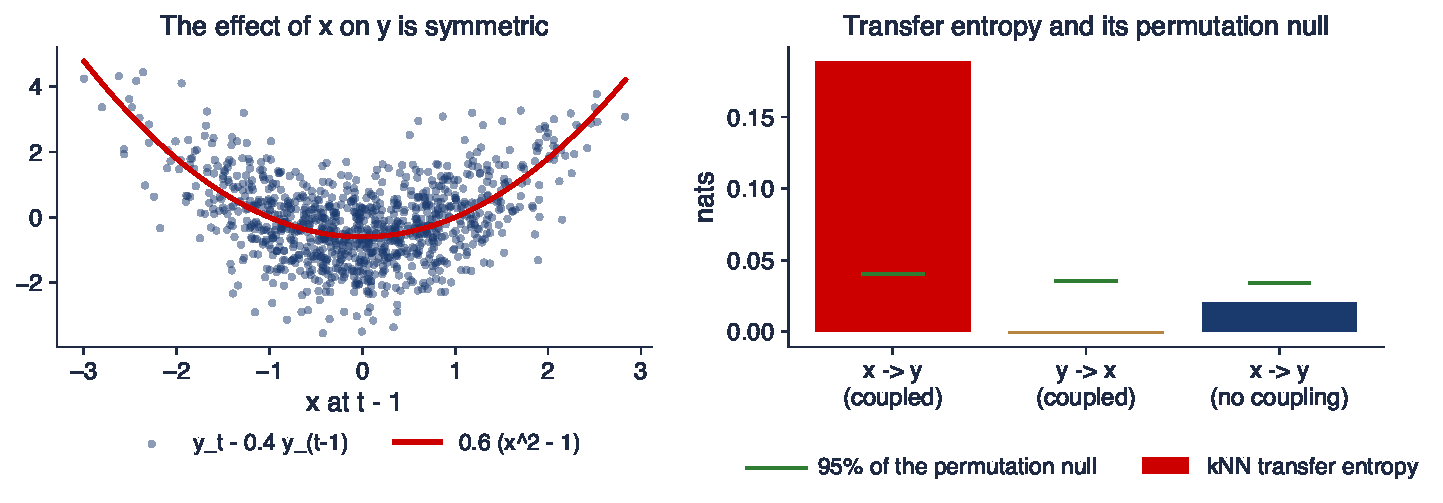
\includegraphics[width=0.97\textwidth,height=0.5\textheight,keepaspectratio]{ats_ch14_te.pdf}
\end{center}
\vspace{-0.25cm}
\begin{itemize}
    \item Simulated: $y_t = 0.4y_{t-1} + 0.6(x_{t-1}^2 - 1) + u_t$, $x$ a Gaussian AR(1) with unit variance, $u_t$ standard Normal noise, $T = 1\,000$
    \item $x_{t-1}^2 - 1$ has mean zero and no correlation with $x_{t-1}$; kNN TE with $k = 5$ neighbours, 199 block permutations
\end{itemize}
\quantlet{ATS\_ch14\_granger}{\qlurl{ATS_ch14_granger}}
\end{frame}

\begin{frame}{Interpreting transfer entropy}
\itemsize{\small}
\begin{itemize}
    \item Linear Granger: p-value 0.86; Gaussian TE 0.05$\times10^{-3}$ nats: the symmetric effect averages out in a linear regression
    \item kNN TE $x\to y$: 0.189 nats, permutation $p$ 0.005; reverse direction \ensuremath{-}0.001 ($p$ 0.76); without coupling 0.021 ($p$ 0.26)
    \item On the markets of the previous slide the Gaussian TE from the S\&P 500 to the BET is 6.1$\times10^{-3}$ nats: significant, but tiny as information
    \item TE needs much more data than Granger and a careful choice of $k$, history lengths and permutation blocks; pre-register them
\end{itemize}
\end{frame}

\begin{frame}{Recap: Granger causality and causal effects}
\itemsize{\small}
\begin{itemize}
    \item Granger causality is incremental predictability relative to an information set; enlarging the set can create or destroy it
    \item A causal effect needs potential outcomes, non-anticipation and an assignment that is as good as random given the past
    \item Transfer entropy extends Granger to distributions; for Gaussian processes the two coincide
\end{itemize}
\end{frame}


%=============================================================================
\section{Causal discovery in time series}
%=============================================================================

\begin{frame}{Time series graphs (1/2)}
\itemsize{\small}
\begin{itemize}
    \item \textbf{Nodes} $X^i_t$: variable $i$ at time $t$; an \textbf{arrow} $X^i_{t-\tau}\to X^j_t$ when $X^i_{t-\tau}$ is a direct cause of $X^j_t$ given the rest of the past \refRunE
    \begin{itemize}
        \item $\tau \ge 1$: the lag of the link; $\tau_{\max}$: the largest lag considered
        \item the graph is the same at every $t$ (causal stationarity); arrows only go forward in time
    \end{itemize}
    \item Three assumptions turn independences into arrows \refSGS
    \begin{itemize}
        \item \textbf{causal Markov}: each variable is independent of its non-effects given its parents (direct causes)
        \item \textbf{faithfulness}: no independence arises by cancellation of effects
        \item \textbf{causal sufficiency}: no hidden common causes
    \end{itemize}
\end{itemize}
\end{frame}

\begin{frame}{Time series graphs (2/2)}
\itemsize{\small}
\begin{itemize}
    \item Under these assumptions an arrow is a conditional dependence given the whole past \[ X^i_{t-\tau}\to X^j_t \iff X^i_{t-\tau} \not\perp X^j_t \mid \mathbf X^-_t\setminus\{X^i_{t-\tau}\} \]
    \begin{itemize}
        \item $\perp$: independence ($\not\perp$: dependence); $\mathbf X^-_t$: all variables at lags $1, \dots, \tau_{\max}$ before $t$
        \item this is the full conditional (VAR) Granger test
    \end{itemize}
    \item With $N$ variables and $\tau_{\max}$ lags the conditioning set has $N\tau_{\max}$ elements
    \begin{itemize}
        \item the power of the test collapses in high dimension: the motivation for PCMCI
    \end{itemize}
\end{itemize}
\end{frame}

\begin{frame}{PCMCI}
\itemsize{\small}
\begin{itemize}
    \item \refPCMCI: two steps, each a sequence of conditional independence tests (partial correlation here; nonlinear tests possible)
    \item \textbf{PC1} (condition selection), for each $X^j_t$
    \begin{itemize}
        \item start from all lagged candidates; remove those independent of $X^j_t$ given the $p$ strongest others, $p = 1, 2, \dots$
        \item the result $\hat{\mathcal P}(X^j_t)$ is a superset of the parents of $X^j_t$
    \end{itemize}
    \item \textbf{MCI} (momentary conditional independence): test each link given the parents of both ends \[ X^i_{t-\tau} \perp X^j_t \mid \hat{\mathcal P}(X^j_t)\setminus\{X^i_{t-\tau}\},\ \hat{\mathcal P}(X^i_{t-\tau}) \]
    \begin{itemize}
        \item conditioning on the parents of the \textbf{source} $X^i_{t-\tau}$ removes its autocorrelation: false positives stay near $\alpha$
        \item conditioning sets stay small, so power is kept in high dimension
    \end{itemize}
    \item Hidden confounders, contemporaneous links, nonstationarity and measurement error break the guarantees; the output is a hypothesis about a graph
\end{itemize}
\end{frame}

\begin{frame}{PCMCI against correlation and the full VAR}
\itemsize{\footnotesize}
\begin{center}
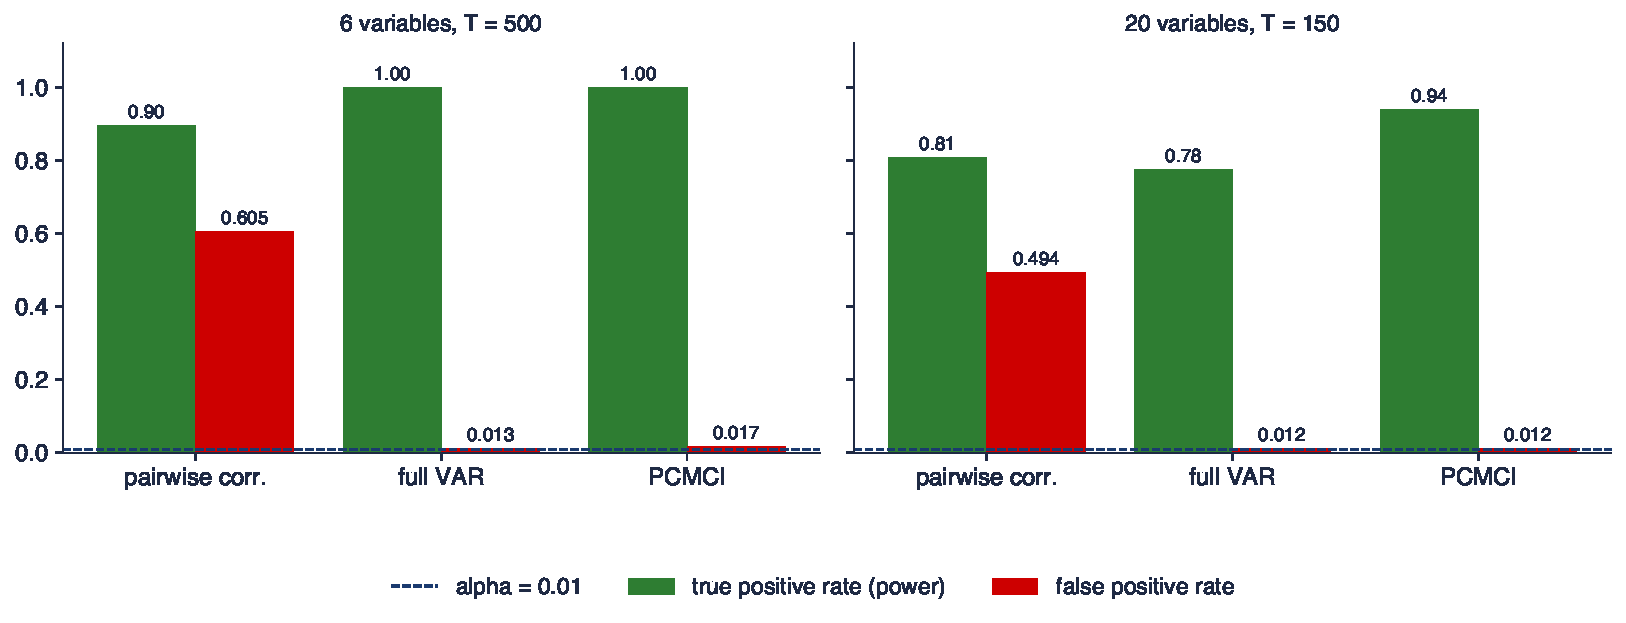
\includegraphics[width=0.97\textwidth,height=0.56\textheight,keepaspectratio]{ats_ch14_pcmci_sim.pdf}
\end{center}
\vspace{-0.25cm}
\begin{itemize}
    \item A known lagged system (a persistent common driver, chains and a collider), $\tau_{\max} = 3$, $\alpha = 0.01$, 50 replications; right: 14 extra independent AR(1) series
\end{itemize}
\quantlet{ATS\_ch14\_discovery}{\qlurl{ATS_ch14_discovery}}
\end{frame}

\begin{frame}{Interpreting the discovery experiment}
\itemsize{\small}
\begin{itemize}
    \item Lagged correlations find most true links but flag 0.605 of the absent ones: autocorrelation and the common driver make everything correlated
    \item Six variables, $T = 500$: the full VAR and PCMCI are equivalent (power 1.00 and 1.00; false positives 0.013 and 0.017)
    \item Twenty variables, $T = 150$: the VAR conditions on 60 regressors and its power falls to 0.78; PCMCI keeps 0.94 with false positives 0.012
    \item The advantage of PCMCI is a high-dimensional one; in small systems a well-specified VAR is enough
\end{itemize}
\end{frame}

\begin{frame}{A discovered graph of market volatility}
\itemsize{\footnotesize}
\begin{center}
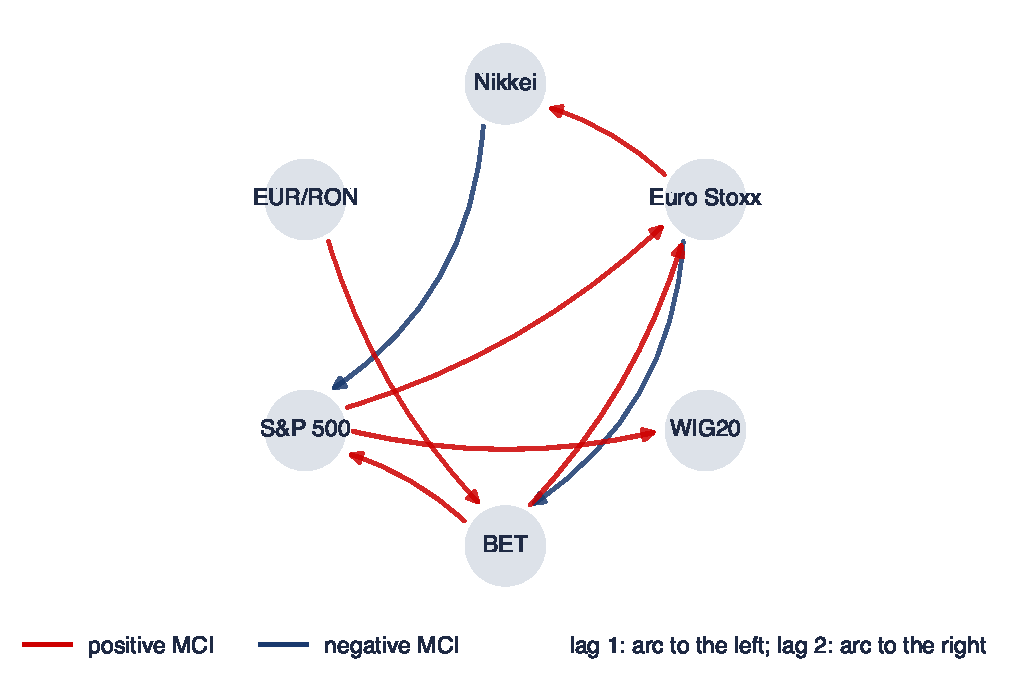
\includegraphics[width=0.97\textwidth,height=0.58\textheight,keepaspectratio]{ats_ch14_pcmci_vol.pdf}
\end{center}
\vspace{-0.25cm}
\begin{itemize}
    \item PCMCI on weekly log realised variances (sum of squared daily returns), 13 January 2008 -- 20 September 2026, $T = 973$ weeks, $\tau_{\max} = 2$, $\alpha = 0.01$; weeks remove the ordering of daily closes
\end{itemize}
\quantlet{ATS\_ch14\_discovery}{\qlurl{ATS_ch14_discovery}}
\end{frame}

\begin{frame}{Interpreting the volatility graph}
\itemsize{\small}
\begin{itemize}
    \item Lagged correlation tests are significant for 56 of the 60 possible lagged cross links; PCMCI keeps 8
    \item Volatility is a common factor: most of the raw dependence is explained by each market's own past and by the shared global shock within the week
    \item The surviving arrows are small partial correlations; contemporaneous spillovers within the week are invisible to a lagged-only analysis
    \item A hidden global factor (news, VIX) violates causal sufficiency: read the graph as a map of predictive links, not of spillover mechanisms
\end{itemize}
\end{frame}

\begin{frame}{Convergent cross mapping}
\itemsize{\footnotesize}
\begin{columns}[T]
\begin{column}{0.3\textwidth}
\centering

\includegraphics[height=0.42\textheight]{ch14_sugihara_2015.jpg}\\[1mm]
\imgcap{George Sugihara}
\imgcredit{https://commons.wikimedia.org/wiki/File:Sugihara_George.png}{Photo: J Park (2015); CC BY-SA 4.0; Wikimedia Commons}
\end{column}
\begin{column}{0.68\textwidth}
\begin{itemize}
    \item Deterministic coupled dynamics: Granger's separability fails, because the information of the cause is already in the effect \refSug
    \item Takens \refTak: the delay vectors of $y$ reconstruct the attractor of the whole system \[ M_y = \{(y_t, y_{t-\tau}, \dots, y_{t-(E-1)\tau})\} \]
    \begin{itemize}
        \item $E$: the embedding dimension; $\tau$: the delay between coordinates
    \end{itemize}
    \item If $x$ drives $y$, the neighbours of a point on $M_y$ identify $x_t$: \textbf{cross-map} $x$ from $M_y$
    \begin{itemize}
        \item simplex projection: a weighted average of $x$ at the $E + 1$ nearest neighbours; skill: the correlation $\rho$ between estimate and truth
    \end{itemize}
    \item Criterion: the skill must \textbf{converge} (increase) with the library size $L$, the number of points used to build $M_y$
    \item Note the direction: skill of $M_y \to x$ is evidence for $x \to y$
\end{itemize}
\end{column}
\end{columns}
\end{frame}

\begin{frame}{Cross mapping: a coupling and a common forcing}
\itemsize{\footnotesize}
\begin{center}
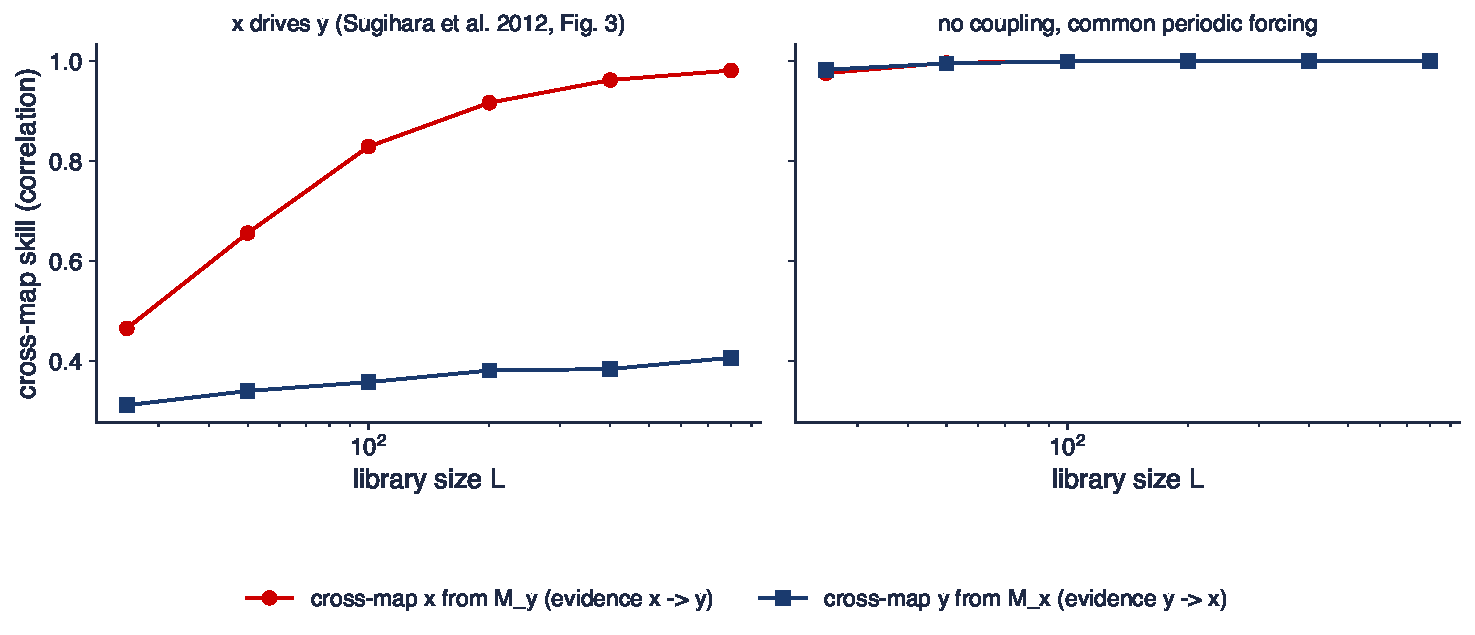
\includegraphics[width=0.97\textwidth,height=0.48\textheight,keepaspectratio]{ats_ch14_ccm.pdf}
\end{center}
\vspace{-0.25cm}
\begin{itemize}
    \item Coupled logistic maps of \refSug: $x_{t+1} = x_t(r_x - r_xx_t - \beta_{xy}y_t)$, $y_{t+1} = y_t(r_y - r_yy_t - \beta_{yx}x_t)$
    \item $r_x = 3.8$, $r_y = 3.5$: growth rates (chaotic regime); $\beta_{yx} = 0.32$: effect of $x$ on $y$; $\beta_{xy} = 0$: no effect of $y$ on $x$; right: two uncoupled maps with the same periodic forcing; $E = 2$
\end{itemize}
\quantlet{ATS\_ch14\_discovery}{\qlurl{ATS_ch14_discovery}}
\end{frame}

\begin{frame}{Interpreting cross mapping}
\itemsize{\small}
\begin{itemize}
    \item Left: skill for $x\to y$ rises from 0.47 ($L = 25$) to 0.98 ($L = 800$); the reverse stays near 0.41: the published pattern
    \item Right: no coupling at all, yet both directions reach 0.999 and 0.999: a shared periodic driver synchronises the maps and CCM reports bidirectional causality
    \item Known critiques: seasonality and synchrony \refBaC, noise and external forcing \refMon, the choice of lag \refYDGS
    \item Use CCM for low-noise nonlinear systems, with surrogate tests that preserve seasonality; never as a black-box causality detector for economic series
\end{itemize}
\end{frame}

\begin{frame}{Recap: Causal discovery}
\itemsize{\small}
\begin{itemize}
    \item A discovered graph is only as good as causal Markov, faithfulness and sufficiency; hidden common drivers are the rule in economics
    \item PCMCI controls false positives under autocorrelation and keeps power in high dimension
    \item CCM targets deterministic coupling; synchrony and common forcing produce false bidirectional links
\end{itemize}
\end{frame}


%=============================================================================
\section{Interrupted time series and event studies}
%=============================================================================

\begin{frame}{Interrupted time series (1/2)}
\itemsize{\small}
\begin{itemize}
    \item One series, an intervention at $T_0$ \refLCG; step 1: model the pre-period \[ y_t = f(t, \text{season}, x_t; \theta) + u_t, \qquad t \le T_0 \]
    \begin{itemize}
        \item $f$: trend, seasonal effects and covariates $x_t$, with parameters $\theta$; $u_t$: the error
    \end{itemize}
    \item Step 2: the effect is the gap between the outcome and the extrapolated model \[ \hat\tau_t = y_t - f(t, \cdot\,; \hat\theta), \qquad t > T_0 \]
    \begin{itemize}
        \item segmented regression is the special case with level and slope dummies after $T_0$
    \end{itemize}
    \item \textbf{Identification}
    \begin{itemize}
        \item nothing else changes at $T_0$; the pre-period model would have continued; no anticipation
    \end{itemize}
\end{itemize}
\end{frame}

\begin{frame}{Interrupted time series (2/2)}
\itemsize{\small}
\begin{itemize}
    \item \textbf{Inference with dependent errors}: the variance of the cumulative effect over $n$ periods \[ \mathrm{Var}\Big(\sum_{t=T_0+1}^{T_0+n}\hat\tau_t\Big) \approx n\,\Omega + a'\hat V_\theta a \]
    \begin{itemize}
        \item $\Omega$: the long-run variance of $u_t$ (\atschlink{https://danpele.github.io/Advanced-Time-Series/EN/Courses/chapter0_refresher_inference.pdf}{Chapter 0}); $\hat V_\theta$: the covariance of $\hat\theta$; $a$: the sum of the regressors of $f$ over the $n$ periods
        \item first term: noise of the outcomes; second term: estimation error of the counterfactual
    \end{itemize}
    \item With AR(1) errors, autocorrelation $\rho$ and $\sigma^2 = \mathrm{Var}(u_t)$ \[ \Omega = \sigma^2\,\frac{1 + \rho}{1 - \rho} \]
    \begin{itemize}
        \item i.i.d.\ standard errors are too small by the factor $\sqrt{(1 + \rho)/(1 - \rho)}$, e.g.\ 1.7 for $\rho = 0.5$
    \end{itemize}
\end{itemize}
\end{frame}

\begin{frame}{Romania 2025: two measures one month apart}
\itemsize{\small}
\begin{columns}[T]
\begin{column}{0.4\textwidth}
\centering
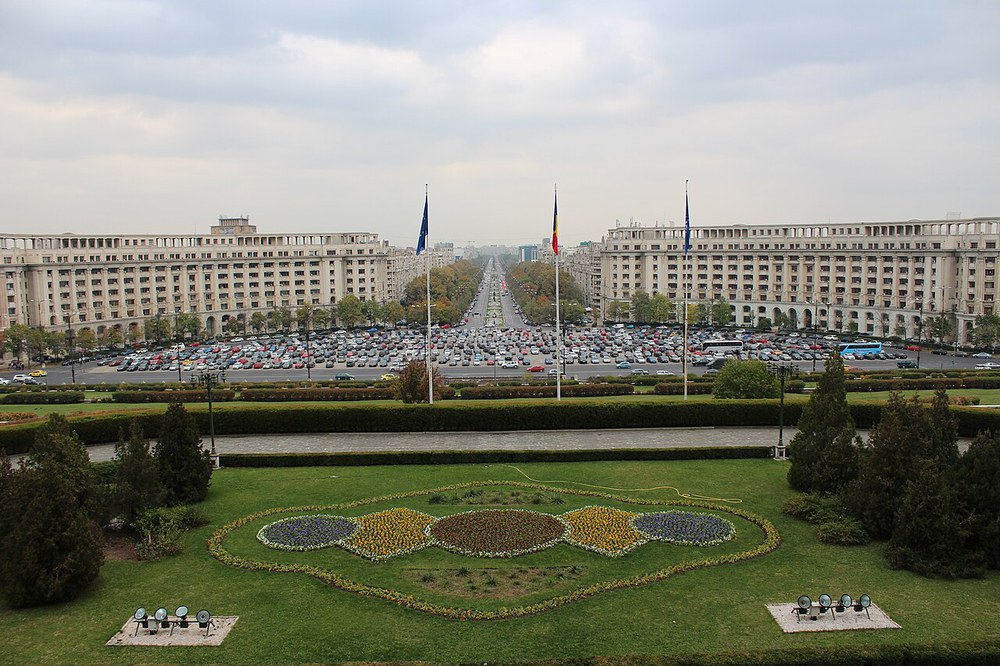
\includegraphics[height=0.40\textheight]{ch14_parliament_bucharest_2017.jpg}\\[1mm]
\imgcap{Palace of the Parliament, Bucharest}
\imgcredit{https://commons.wikimedia.org/wiki/File:Palace_of_the_Parliament_in_Bucharest_(51878975552).jpg}{Photo: William John Gauthier (2017); CC BY-SA 2.0; Wikimedia Commons}
\end{column}
\begin{column}{0.58\textwidth}
\begin{itemize}
    \item \textbf{1 July 2025}
    \begin{itemize}
        \item the cap on household electricity prices (in force since 2022) ends
        \item the household gas cap continues
    \end{itemize}
    \item \textbf{7 July 2025}
    \begin{itemize}
        \item the government assumes responsibility for a fiscal package in Parliament (Law 141/2025, published 25 July)
    \end{itemize}
    \item \textbf{1 August 2025}
    \begin{itemize}
        \item standard VAT 19\% $\to$ 21\%; reduced rates 5\% and 9\% $\to$ 11\%; excise duties up
    \end{itemize}
    \item Timing alone cannot separate the two; the HICP at constant tax rates can isolate the tax part
    \item Question: how much did the two measures add to Romanian inflation over the following year?
\end{itemize}
\end{column}
\end{columns}
\end{frame}

\begin{frame}{An interrupted time series for Romanian inflation}
\itemsize{\footnotesize}
\begin{center}
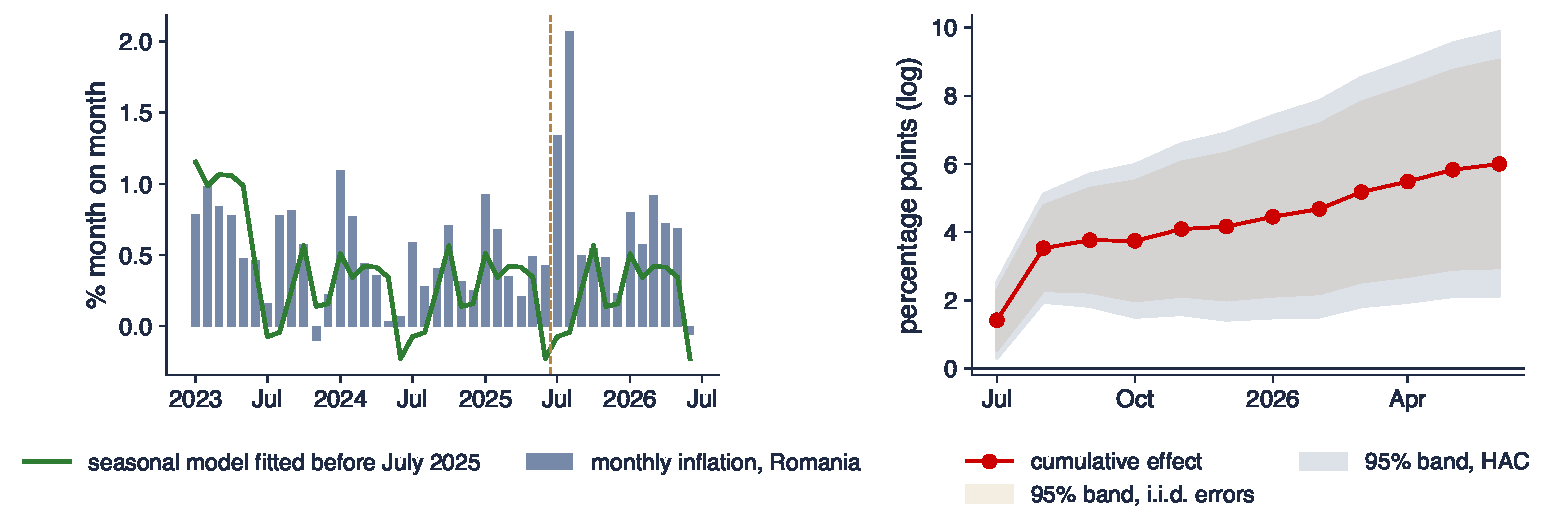
\includegraphics[width=0.97\textwidth,height=0.56\textheight,keepaspectratio]{ats_ch14_its.pdf}
\end{center}
\vspace{-0.25cm}
\begin{itemize}
    \item Monthly HICP inflation (log change); pre-period model: 12 month effects and a step for July 2021 -- June 2023, fitted on 126 months to June 2025; effects July 2025 -- June 2026
\end{itemize}
\quantlet{ATS\_ch14\_its\_event}{\qlurl{ATS_ch14_its_event}}
\end{frame}

\begin{frame}{Interpreting the interrupted time series}
\itemsize{\small}
\begin{itemize}
    \item July 2025: +1.41 pp above the seasonal norm; August 2025: +2.11 pp; later months +0.25 pp on average
    \item Cumulative effect over twelve months 6.0 pp; standard error 1.55 with i.i.d. errors, 1.98 with HAC (residual autocorrelation 0.33, long-run variance 1.63 times $\sigma^2$)
    \item The ITS counterfactual is Romania's own seasonal norm: it ignores everything else that happened in Europe after June 2025
    \item A control group is needed to remove common shocks: the synthetic control of Section 5 uses 26 EU countries
\end{itemize}
\end{frame}

\begin{frame}{Event studies with dependent errors}
\itemsize{\small}
\begin{itemize}
    \item \refMac, the \textbf{market model} estimated on days $[-250, -11]$ before the event \[ r_t = \alpha + \beta r^m_t + \varepsilon_t, \qquad AR_t = r_t - \hat\alpha - \hat\beta r^m_t, \qquad CAR[0, k] = \sum_{t=0}^k AR_t \]
    \begin{itemize}
        \item $r_t$: the return of the asset; $r^m_t$: the market return; $AR_t$: the abnormal return; $CAR[0, k]$: the cumulative abnormal return over days 0 to $k$
    \end{itemize}
    \item Variance of the CAR
    \begin{itemize}
        \item $(k + 1)\sigma^2$ under i.i.d.\ errors; $(k + 1)\Omega$ with serial correlation ($\Omega$: long-run variance)
        \item event-induced variance and clustered events need cross-sectional or bootstrap corrections
    \end{itemize}
    \item Identification: the event is a surprise on day 0 and nothing else happened
    \begin{itemize}
        \item anticipated news is priced before the window
    \end{itemize}
    \item Here: the BET index against the Euro Stoxx 50, four Romanian political and fiscal events of 2024--2025, window $[0, 2]$
\end{itemize}
\end{frame}

\begin{frame}{Romanian stocks around political and fiscal news}
\itemsize{\footnotesize}
\begin{center}
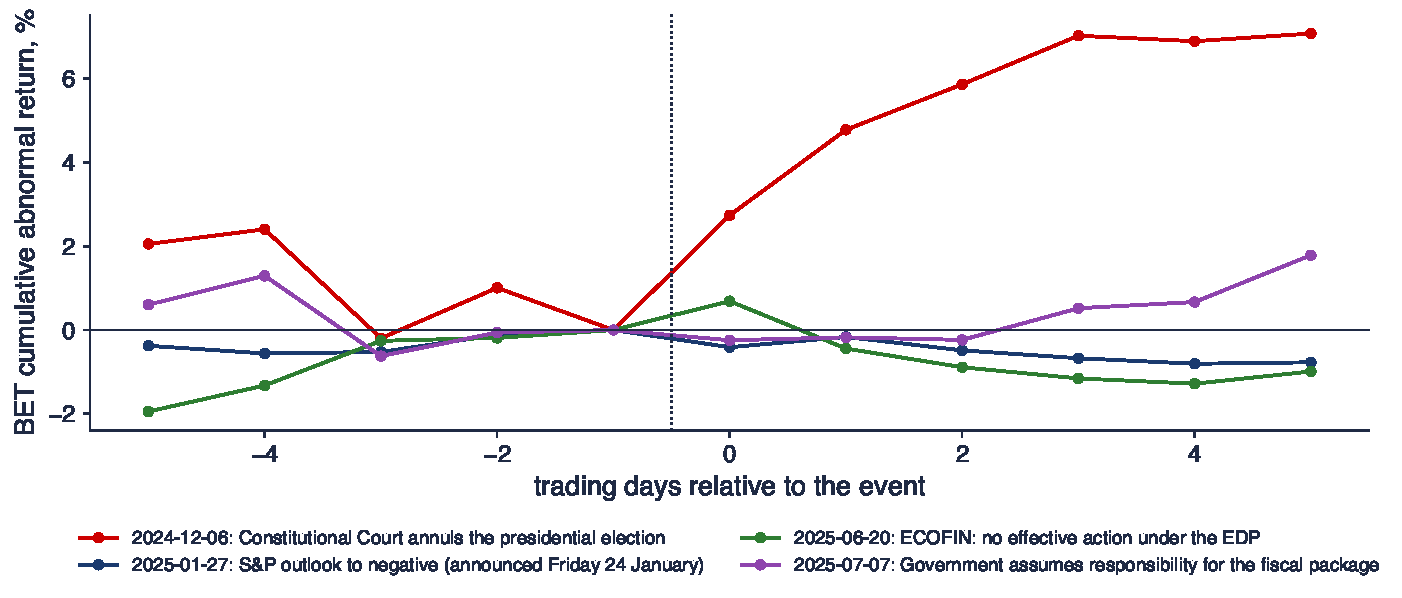
\includegraphics[width=0.97\textwidth,height=0.54\textheight,keepaspectratio]{ats_ch14_event.pdf}
\end{center}
\vspace{-0.25cm}
\begin{itemize}
    \item Cumulative abnormal return of the BET, normalised at day $-1$; market model on the Euro Stoxx 50; rating actions announced after the close on a Friday are dated on the next Monday
\end{itemize}
\quantlet{ATS\_ch14\_its\_event}{\qlurl{ATS_ch14_its_event}}
\end{frame}

\begin{frame}{Interpreting the event study}
\itemsize{\small}
\begin{itemize}
    \item Annulment of the presidential election (6 December 2024): CAR[0, 2] +5.9\%, $t$ = 5.25 (i.i.d.) and 5.08 (HAC): the market priced a lower political risk
    \item S\&P negative outlook: \ensuremath{-}0.5\% ($t$ = \ensuremath{-}0.33); ECOFIN decision: \ensuremath{-}0.9\% ($t$ = \ensuremath{-}0.52); fiscal package: \ensuremath{-}0.2\% ($t$ = \ensuremath{-}0.14)
    \item Fiscal news had been discussed for months: no surprise on day 0, no abnormal return; a null result here says nothing about the economic effect of the measures
    \item HAC and i.i.d.\ standard errors are close for daily returns (little autocorrelation); they differ for monthly macro data (previous section)
\end{itemize}
\end{frame}

\begin{frame}{Recap: Interrupted time series and event studies}
\itemsize{\small}
\begin{itemize}
    \item ITS and event studies compare a series with its own extrapolated past: valid only if nothing else changed at the same time
    \item Cumulative effects need the long-run variance of the errors, not $\sigma^2$
    \item Anticipation moves the effect before the window: dating the news is part of the identification
\end{itemize}
\end{frame}


%=============================================================================
\section{Synthetic control}
%=============================================================================

\begin{frame}{The synthetic control estimator (1/2)}
\itemsize{\small}
\begin{itemize}
    \item Units: $j = 1$ treated, $j = 2, \dots, J + 1$ the \textbf{donor pool}; treatment after period $T_0$ \refAbG, \refADHa
    \begin{itemize}
        \item $Y_{jt}(1)$, $Y_{jt}(0)$: potential outcomes of unit $j$ at $t$ with and without the treatment
    \end{itemize}
    \item Target: the effect on the treated unit after $T_0$ \[ \tau_{1t} = Y_{1t}(1) - Y_{1t}(0), \qquad t > T_0 \]
    \begin{itemize}
        \item $Y_{1t}(1) = Y_{1t}$ is observed; $Y_{1t}(0)$ must be estimated
    \end{itemize}
    \item \textbf{Synthetic control}: a weighted average of the donors stands in for $Y_{1t}(0)$ \[ \hat Y_{1t}(0) = \sum_{j=2}^{J+1} w_jY_{jt}, \qquad \hat\tau_{1t} = Y_{1t} - \hat Y_{1t}(0) \]
    \begin{itemize}
        \item $w_j \ge 0$: the weight of donor $j$, with $\sum_j w_j = 1$
    \end{itemize}
\end{itemize}
\end{frame}

\begin{frame}{The synthetic control estimator (2/2)}
\itemsize{\small}
\begin{itemize}
    \item \textbf{Weights}: the convex combination of donors closest to the treated unit in the pre-treatment predictors \[ w^*(V) = \arg\min_w\, (X_1 - X_0w)'V(X_1 - X_0w), \qquad w_j \ge 0,\ \sum_j w_j = 1 \]
    \begin{itemize}
        \item $X_1$: the vector of pre-treatment predictors of the treated unit (outcome averages, covariates); $X_0$: the matrix of the same predictors for the donors
        \item a quadratic programme on the simplex: weights are sparse and interpretable; no extrapolation outside the donors' range
    \end{itemize}
    \item $V = \mathrm{diag}(v)$: the importance of each predictor
    \begin{itemize}
        \item chosen to minimise the pre-period $\mathrm{MSPE} = \frac{1}{T_0}\sum_{t \le T_0}(Y_{1t} - \sum_j w_j^*(V)Y_{jt})^2$ (nested optimisation, \refADHs)
        \item MSPE: mean squared prediction error of the outcome; alternative: cross-validation on a training and a validation period \refADHb
        \item with all pre-period outcomes in $X$, the covariates get no weight \refKKPS
    \end{itemize}
\end{itemize}
\end{frame}

\begin{frame}{Why it works: the factor model}
\itemsize{\small}
\begin{itemize}
    \item \refADHa: the untreated outcomes follow a factor model (interactive fixed effects \refBai) \[ Y_{jt}(0) = \delta_t + \theta_tZ_j + \lambda_t\mu_j + \varepsilon_{jt} \]
    \begin{itemize}
        \item $\delta_t$: a common time effect; $Z_j$: observed covariates with time-varying coefficients $\theta_t$; $\lambda_t$: unobserved common factors; $\mu_j$: unobserved loadings of unit $j$; $\varepsilon_{jt}$: transitory shocks
        \item DiD assumes $\lambda_t$ constant (parallel trends); SC lets the common factors vary over time
    \end{itemize}
    \item If the weights reproduce the treated unit before $T_0$, $\sum_j w_jY_{jt} = Y_{1t}$ for all $t \le T_0$ and $\sum_j w_jZ_j = Z_1$, then
    \begin{itemize}
        \item the bias of $\hat\tau_{1t}$ is bounded by a term that \textbf{shrinks as $T_0$ grows}, relative to the scale of $\varepsilon$ (\atsapplink{atsapp1}{atssrc2}{Appendix})
        \item a good fit over a long pre-period is evidence that the loadings $\mu_j$ are matched
    \end{itemize}
    \item A short pre-period with a perfect fit can be overfitting the noise: the bound is then weak \refAba
\end{itemize}
\end{frame}

\begin{frame}{Feasibility conditions}
\itemsize{\small}
\begin{itemize}
    \item \textbf{Convex hull} \refAba
    \begin{itemize}
        \item the treated unit must lie inside the range of the donors; otherwise no convex combination fits it
    \end{itemize}
    \item \textbf{Donor pool}
    \begin{itemize}
        \item units with similar structure, not affected by the treatment (no spillovers), without large shocks of their own after $T_0$
    \end{itemize}
    \item \textbf{No anticipation}
    \begin{itemize}
        \item effects must not start before $T_0$; backdate $T_0$ to the announcement if needed
    \end{itemize}
    \item \textbf{Long pre-period} with a good fit
    \begin{itemize}
        \item \textbf{interpolation bias}: a mix of very different donors may not resemble the treated unit even if the averages match
    \end{itemize}
    \item Report
    \begin{itemize}
        \item weights, predictor balance, pre-period RMSPE, the placebo distribution, leave-one-out
    \end{itemize}
\end{itemize}
\end{frame}

\begin{frame}{Inference with one treated unit}
\itemsize{\small}
\begin{itemize}
    \item \textbf{In-space placebos} \refADHa: reassign the treatment to every donor in turn, refit, and compute the ratio \[ r_j = \mathrm{RMSPE}_{\mathrm{post}}/\mathrm{RMSPE}_{\mathrm{pre}}, \qquad \text{p-value} = \#\{j: r_j \ge r_1\}/(J + 1) \]
    \begin{itemize}
        \item RMSPE: root mean squared prediction error of the synthetic control, before (pre) and after (post) $T_0$; a large $r_j$: a large post-treatment gap relative to the pre-fit
        \item $\#\{\cdot\}$: the number of units; the smallest attainable p-value is $1/(J + 1)$; exact only under random assignment across units, otherwise a descriptive ranking \refFiP
    \end{itemize}
    \item \textbf{Other robustness checks}
    \begin{itemize}
        \item in-time placebos: a fictitious $T_0$ inside the pre-period should give no effect
        \item leave-one-out: drop each donor with positive weight and refit
    \end{itemize}
    \item \textbf{Conformal inference} \refCWZ: test $H_0$: $\tau_{1t} = \tau_0$ by permuting the residuals over time
    \begin{itemize}
        \item block permutations for dependence; confidence sets by inverting the test over $\tau_0$
    \end{itemize}
\end{itemize}
\end{frame}

\begin{frame}{Case study: the economic cost of German reunification}
\itemsize{\small}
\begin{columns}[T]
\begin{column}{0.38\textwidth}
\centering
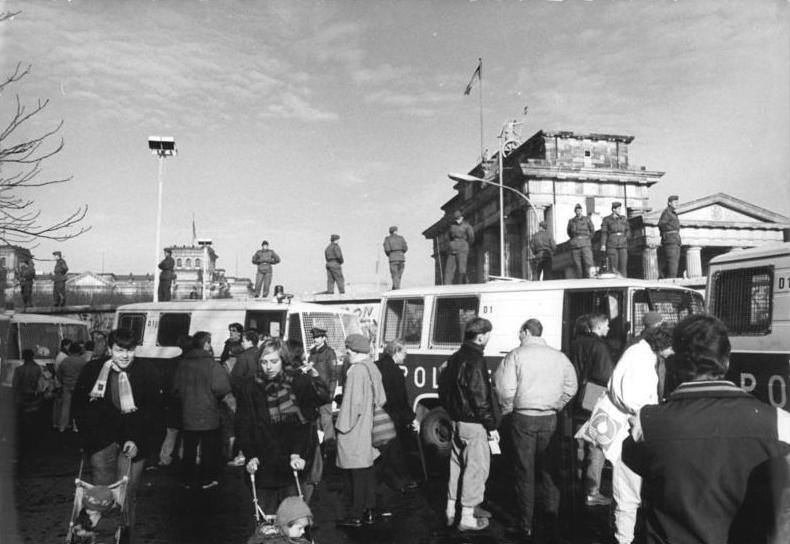
\includegraphics[height=0.42\textheight]{ch14_brandenburg_gate_1989.jpg}\\[1mm]
\imgcap{Brandenburg Gate, Berlin, 11 November 1989}
\imgcredit{https://commons.wikimedia.org/wiki/File:Bundesarchiv_Bild_183-1989-1111-009,_Berlin,_Brandenburger_Tor,_Polizeiabsperrung.jpg}{Photo: Peer Grimm, Bundesarchiv Bild 183-1989-1111-009 (1989); CC BY-SA 3.0 de; Wikimedia Commons}
\end{column}
\begin{column}{0.6\textwidth}
\begin{itemize}
    \item \refADHb
    \begin{itemize}
        \item did the 1990 reunification lower West German GDP per capita?
    \end{itemize}
    \item Data \refADHd
    \begin{itemize}
        \item West Germany and 16 OECD countries, 1960--2003
        \item predictors: GDP per capita, trade openness, inflation, industry share, schooling, investment rate
    \end{itemize}
    \item $V$ by cross-validation (Section 4 and the replication code)
    \begin{itemize}
        \item training predictors 1971--1980, validation outcomes 1981--1990
        \item final weights from the 1981--1990 predictors with that $V$
    \end{itemize}
    \item Erratum (2026)
    \begin{itemize}
        \item the outcome is GDP per capita in PPP \textit{current} USD, not 2002 USD as labelled in the article
    \end{itemize}
\end{itemize}
\end{column}
\end{columns}
\end{frame}

\begin{frame}{Replication: weights and predictor balance}
\itemsize{\small}
\begin{columns}[T]
\begin{column}{0.38\textwidth}
\begin{center}
\footnotesize
\begin{tabular}{lrr}
\toprule
\textbf{Donor} & \textbf{ours} & \textbf{ADH, Table 1} \\
\midrule
Austria & 0.42 & 0.42 \\
United States & 0.22 & 0.22 \\
Japan & 0.16 & 0.16 \\
Switzerland & 0.11 & 0.11 \\
Netherlands & 0.09 & 0.09 \\
\bottomrule
\end{tabular}
\end{center}

\end{column}
\begin{column}{0.6\textwidth}
\begin{center}
\footnotesize
\begin{tabular}{lrrr}
\toprule
\textbf{Predictor} & \textbf{West Germany} & \textbf{synthetic} & \textbf{OECD avg.} \\
\midrule
GDP per capita & 15809 & 15805 & 13669 \\
Trade openness & 56.8 & 56.9 & 59.8 \\
Inflation & 2.6 & 3.5 & 7.6 \\
Industry share & 34.5 & 34.4 & 33.8 \\
Schooling & 55.5 & 55.3 & 38.7 \\
Investment rate & 27.0 & 27.0 & 25.9 \\
\bottomrule
\end{tabular}
\end{center}

\end{column}
\end{columns}\begin{itemize}
    \item The cross-validated $V$ and the quadratic programme reproduce the published weights to two decimals; all other donors get zero weight
    \item The simple OECD average differs on every predictor: the unweighted comparison would be biased
\end{itemize}
\end{frame}

\begin{frame}{West Germany and its synthetic control}
\itemsize{\footnotesize}
\begin{center}
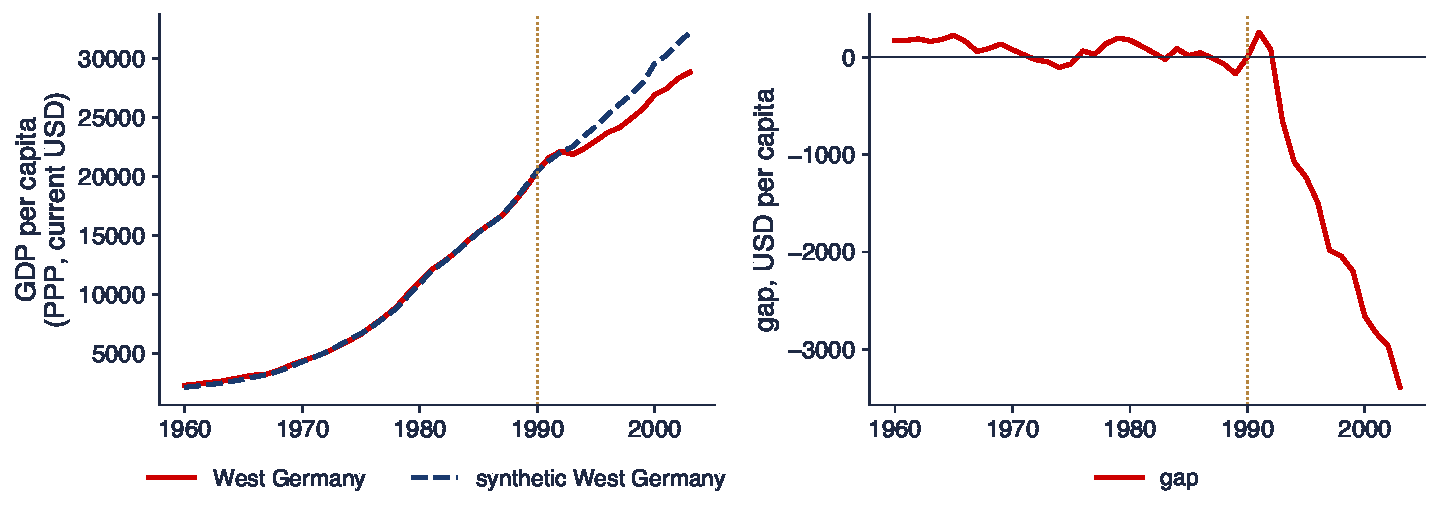
\includegraphics[width=0.97\textwidth,height=0.56\textheight,keepaspectratio]{ats_ch14_germany.pdf}
\end{center}
\vspace{-0.25cm}
\begin{itemize}
    \item Left: GDP per capita (PPP, current USD); right: the gap; pre-1990 RMSPE 121 USD
\end{itemize}
\quantlet{ATS\_ch14\_germany}{\qlurl{ATS_ch14_germany}}
\end{frame}

\begin{frame}{Interpreting the German replication}
\itemsize{\small}
\begin{itemize}
    \item The synthetic West Germany tracks the actual series for thirty years (1960--1989), then grows faster
    \item Average gap 1990--2003: 1588 USD per capita a year (5.6\% of the synthetic level); in 2003: 3391 USD (10.5\%)
    \item The paper reports a reduction of about 1,600 USD a year on average: the replication matches
    \item The donors (Austria, USA, Japan, Switzerland, Netherlands) are rich, industrial economies: the weights make economic sense, a check no algorithm does for us
\end{itemize}
\end{frame}

\begin{frame}{Placebos for the German case}
\itemsize{\footnotesize}
\begin{center}
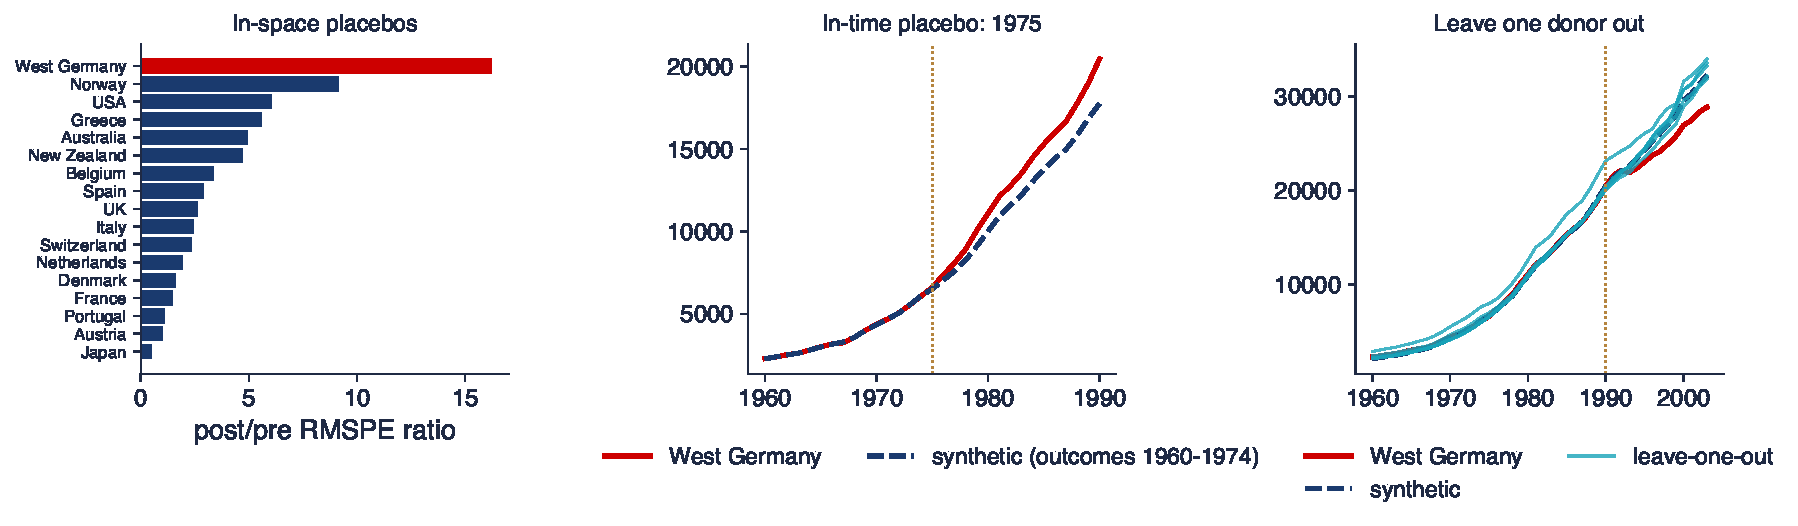
\includegraphics[width=0.97\textwidth,height=0.54\textheight,keepaspectratio]{ats_ch14_germany_placebo.pdf}
\end{center}
\vspace{-0.25cm}
\begin{itemize}
    \item Left: post/pre-1990 RMSPE ratio when each country is treated in turn (ADH 2015, Figure 6); centre: reunification moved to 1975 (as in Figure 4, outcome-only SC); right: one donor left out at a time (Figure 5)
\end{itemize}
\quantlet{ATS\_ch14\_germany}{\qlurl{ATS_ch14_germany}}
\end{frame}

\begin{frame}{Interpreting the German placebos}
\itemsize{\small}
\begin{itemize}
    \item West Germany has the largest ratio (16.2; next: Norway, 9.2): permutation p-value $1/17$ = 0.059, the smallest attainable
    \item Placebo reunification in 1975 (outcome-only SC on 1960--1974, pre-RMSPE 19 USD): West Germany grows faster than its synthetic control (average gap +9.9\% to 1990): no spurious cost appears
    \item With the published 1975 predictors the cross-validated $V$ is not identified: one starting value gives Austria as the donor, the best of eight gives United States \refKPSb
    \item Leaving out any donor keeps a negative gap in 2003, between 2965 and 5138 USD: the result does not hinge on one country
    \item With 17 units the permutation test cannot give $p < 0.059$
\end{itemize}
\end{frame}

\begin{frame}{Case study: the Brexit doppelganger}
\itemsize{\small}
\begin{columns}[T]
\begin{column}{0.3\textwidth}
\centering

\includegraphics[height=0.32\textheight]{ch14_brexit_count_2016.jpg}\\[1mm]
\imgcap{Counting the votes of the EU referendum, 23 June 2016}
\imgcredit{https://commons.wikimedia.org/wiki/File:At_the_Brexit_referendum_count_in_Borehamwood_(28176894300).jpg}{Photo: Steve Bowbrick (2016); CC BY 2.0; Wikimedia Commons}
\end{column}
\begin{column}{0.68\textwidth}
\begin{itemize}
    \item \refBMSS
    \begin{itemize}
        \item the referendum of 23 June 2016 as a natural experiment; outcome: UK real GDP
    \end{itemize}
    \item Design (Section 2.1)
    \begin{itemize}
        \item 23 OECD donors; quarterly real GDP, normalised to 1 in 1995
        \item pre-period 1995Q1--2016Q2; six covariate averages
        \item published weights (Table 2): United States 0.51; Italy 0.17; New Zealand 0.14; Hungary 0.11; Germany 0.05
    \end{itemize}
    \item Published result
    \begin{itemize}
        \item UK output 2.4\% below the doppelganger by the end of 2018
        \item significant by the end-of-sample instability test of \refAnd
    \end{itemize}
    \item Our replication
    \begin{itemize}
        \item the same donors and window; the current OECD vintage (to 2026Q2); the GDP path only (no covariates)
    \end{itemize}
\end{itemize}
\end{column}
\end{columns}
\end{frame}

\begin{frame}{The doppelganger on today's data}
\itemsize{\footnotesize}
\begin{center}
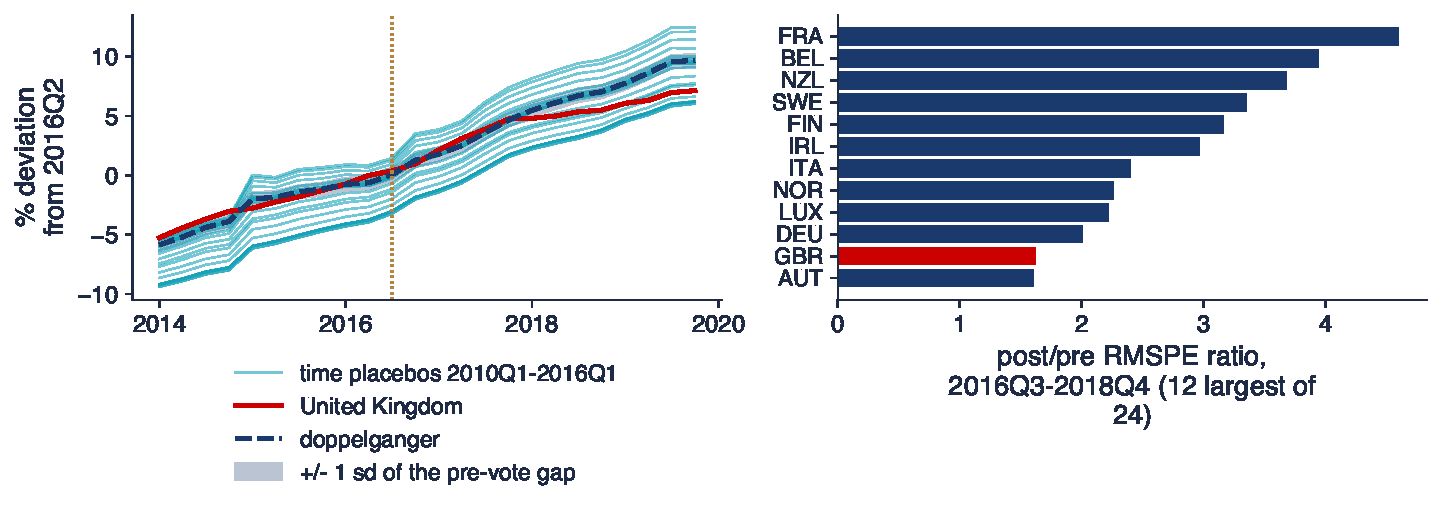
\includegraphics[width=0.97\textwidth,height=0.56\textheight,keepaspectratio]{ats_ch14_brexit.pdf}
\end{center}
\vspace{-0.25cm}
\begin{itemize}
    \item Left: UK real GDP and its doppelganger (\% from 2016Q2), with the doppelgangers of fictitious votes in every quarter 2010Q1--2016Q1; right: the 12 largest post/pre RMSPE ratios of the 24 countries
\end{itemize}
\quantlet{ATS\_ch14\_brexit}{\qlurl{ATS_ch14_brexit}}
\end{frame}

\begin{frame}{Interpreting the Brexit replication}
\itemsize{\small}
\begin{itemize}
    \item Weights on today's data: United States 0.36; Japan 0.19; Canada 0.16; Portugal 0.10; Hungary 0.09; the doppelganger changes with the data vintage
    \item Gap: 0.1\% in 2017Q4, $-$1.5\% in 2018Q4 (published: $-$2.4\%), $-$2.5\% in 2019Q4; pre-vote standard deviation 0.51\%
    \item The UK ranks 11 of 24 in the country placebos; the 25 time placebos give 2018Q4 gaps from \ensuremath{-}4.3\% to 1.9\%: on revised data the evidence is much weaker
    \item A replication changes the data (revisions), the specification (no covariates) and the inference (permutation instead of an end-of-sample test): report each deviation separately
\end{itemize}
\end{frame}

\begin{frame}{Recap: Synthetic control}
\itemsize{\small}
\begin{itemize}
    \item A convex combination of donors fitted on a long pre-period; justified by a factor model; transparent sparse weights
    \item Inference by placebos in space and time, leave-one-out, conformal methods; $p \ge 1/(J + 1)$
    \item German reunification replicates exactly; the Brexit gap is sensitive to data revisions and specification
\end{itemize}
\end{frame}


%=============================================================================
\section{Beyond synthetic control}
%=============================================================================

\begin{frame}{Intercepts and augmentation}
\itemsize{\small}
\begin{itemize}
    \item \textbf{Demeaned SC} \refDI, \refFP: allows a constant level difference $c$ between the treated unit and the donors \[ \hat Y_{1t}(0) = c + \sum_j w_jY_{jt} \]
    \begin{itemize}
        \item the weights are fitted on pre-period outcomes minus the pre-period mean of each unit
        \item solves the level part of the convex-hull problem; consistent under imperfect pre-fit when the factors are stationary \refFP
    \end{itemize}
    \item \textbf{Augmented SC} \refASCM: corrects the SC estimate by the remaining predictor imbalance, through a ridge regression \[ \hat Y^{\mathrm{aug}}_{1t}(0) = \sum_j\hat w_jY_{jt} + \Big(X_1 - \sum_j\hat w_jX_j\Big)'\hat\eta_t \]
    \begin{itemize}
        \item $\hat w_j$: the SC weights; $X_j$: the pre-period outcomes of unit $j$; $\hat\eta_t$: coefficients of a ridge regression of $Y_{jt}$ on $X_j$ across donors, with penalty $\lambda$
        \item equivalent to weights $\hat w + X_0(X_0'X_0 + \lambda I)^{-1}(X_1 - X_0'\hat w)$, which can be negative (controlled extrapolation)
        \item $\lambda \to \infty$ gives SC; $\lambda \to 0$ gives an outcome regression; the bias falls with the remaining imbalance
    \end{itemize}
\end{itemize}
\end{frame}

\begin{frame}{Synthetic difference in differences (1/2)}
\itemsize{\small}
\begin{itemize}
    \item \refSDID: a two-way fixed-effects regression in which units and periods are weighted \[ (\hat\tau, \hat\mu, \hat\alpha, \hat\beta) = \arg\min\sum_{j,t}\big(Y_{jt} - \mu - \alpha_j - \beta_t - W_{jt}\tau\big)^2\hat\omega_j\hat\lambda_t \]
    \begin{itemize}
        \item $W_{jt} = 1$ for the treated unit after $T_0$, 0 otherwise; $\tau$: the effect; $\mu$: the overall mean; $\alpha_j$: unit fixed effects; $\beta_t$: period fixed effects
    \end{itemize}
    \item \textbf{Unit weights} $\hat\omega_j$: SC with an intercept and a ridge penalty
    \begin{itemize}
        \item penalty $\zeta^2T_0\|\omega\|^2$ with $\zeta = (N_{\mathrm{tr}}T_{\mathrm{post}})^{1/4}\hat\sigma$; $N_{\mathrm{tr}}$: treated units; $T_{\mathrm{post}}$: post-periods; $\hat\sigma$: the noise level of the controls
    \end{itemize}
    \item \textbf{Time weights} $\hat\lambda_t$: the pre-periods that best predict the post-period mean of the controls
\end{itemize}
\end{frame}

\begin{frame}{Synthetic difference in differences (2/2)}
\itemsize{\small}
\begin{itemize}
    \item Three estimators as special cases
    \begin{itemize}
        \item DiD: $\omega$ and $\lambda$ uniform
        \item SC: unit weights $\omega$ only (uniform $\lambda$), no unit fixed effect
        \item SDID: both sets of weights, both fixed effects
    \end{itemize}
    \item One treated unit: placebo standard error
    \begin{itemize}
        \item each control in turn plays the treated unit; the standard deviation of the placebo estimates is the standard error (Algorithm 4)
    \end{itemize}
\end{itemize}
\end{frame}

\begin{frame}{Romania 2025: design of the synthetic control}
\itemsize{\small}
\begin{itemize}
    \item Outcome: annual HICP inflation (pp), $100(\ln P_t - \ln P_{t-12})$, Eurostat; treated: Romania; donors: the other 26 EU countries
    \begin{itemize}
        \item $P_t$: the HICP price index in month $t$; pp: percentage points
        \item the annual rate removes seasonality and makes a price-level shock visible for exactly twelve months
    \end{itemize}
    \item Pre-period: July 2023 -- June 2025 (24 months, after the 2021--2023 surge); treatment from July 2025; effect window July 2025 -- June 2026
    \begin{itemize}
        \item a built-in falsification: once the price-level jump leaves the 12-month window (August 2026), the gap must close
    \end{itemize}
    \item Estimators: SC, demeaned SC, ridge-augmented demeaned SC, SDID; inference: in-space placebos
    \item Threats: other countries' own energy and tax measures; anticipation of the VAT increase; Romania outside the donors' range
\end{itemize}
\end{frame}

\begin{frame}{Four counterfactuals for Romanian inflation}
\itemsize{\footnotesize}
\begin{center}
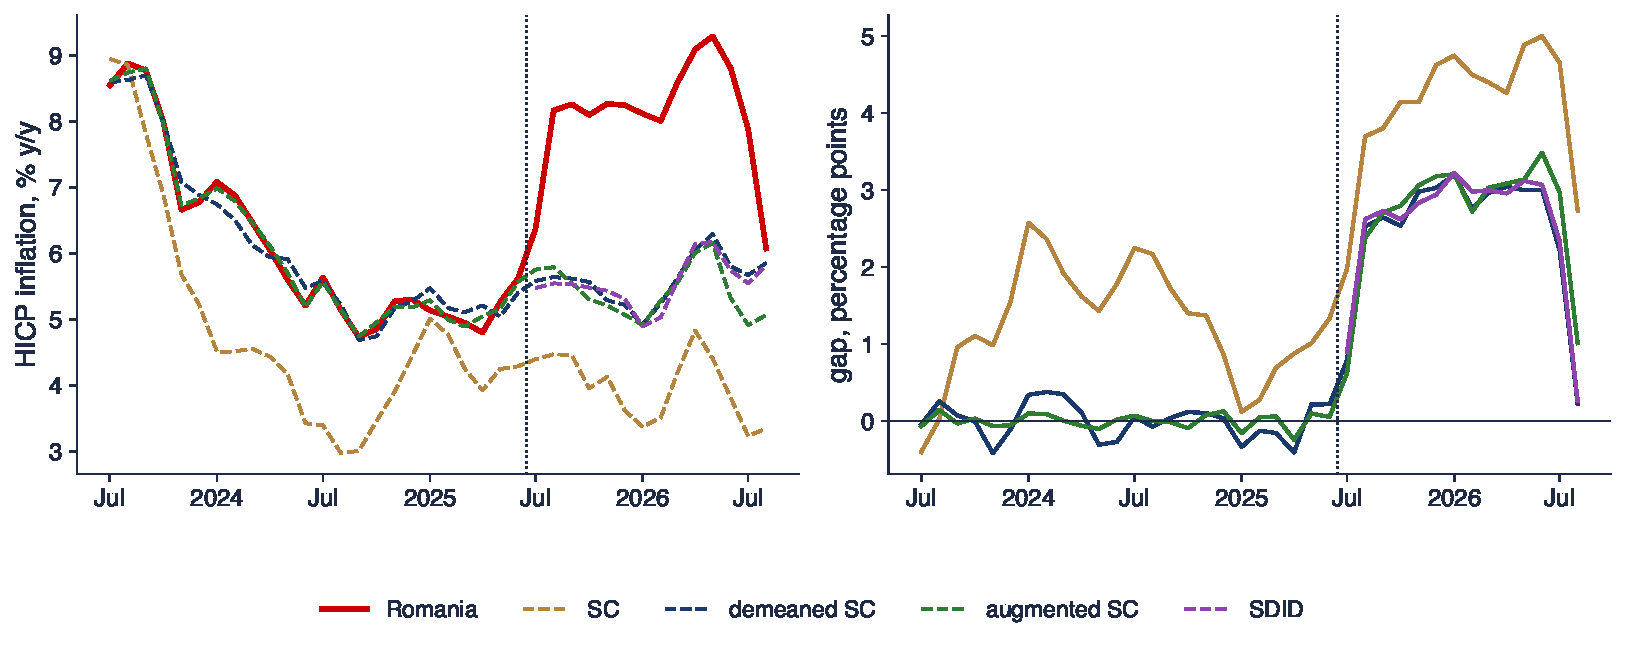
\includegraphics[width=0.97\textwidth,height=0.56\textheight,keepaspectratio]{ats_ch14_ro_sc.pdf}
\end{center}
\vspace{-0.25cm}
\begin{itemize}
    \item Left: Romania and the four estimated counterfactuals; right: the gaps; vertical line: June 2025; data to August 2026
\end{itemize}
\quantlet{ATS\_ch14\_romania}{\qlurl{ATS_ch14_romania}}
\end{frame}

\begin{frame}{Interpreting the four estimators}
\itemsize{\small}
\begin{center}
\scriptsize
\begin{tabular}{lcccc}
\toprule
\textbf{Estimator} & \textbf{pre RMSPE} & \textbf{August 2025} & \textbf{avg. Jul 2025 -- Jun 2026} & \textbf{August 2026} \\
\midrule
SC & 1.45 & 3.70 & 4.18 & 2.73 \\
demeaned SC & 0.23 & 2.53 & 2.70 & 0.22 \\
augmented SC & 0.09 & 2.38 & 2.78 & 1.01 \\
SDID & -- & 2.62 & 2.75 ($se$ 0.70) & 0.26 \\
\bottomrule
\end{tabular}
\end{center}
\begin{itemize}
    \item Classic SC puts all weight on Croatia 0.85; Hungary 0.15: Romania is outside the convex hull, the pre-fit is poor and the effect is overstated
    \item With an intercept the fit is good (weights France 0.38; Slovenia 0.25; Sweden 0.13; Malta 0.10, ...); augmented SC ($\lambda = 1$, 9 negative weights) and SDID agree: 2.7--2.8 pp over twelve months
    \item Falsification: in August 2026 the gap falls to 0.22 (demeaned SC) and 0.26 (SDID); the augmented SC keeps 1.01, the price of extrapolating with negative weights
\end{itemize}
\end{frame}

\begin{frame}{Placebo inference for Romania}
\itemsize{\footnotesize}
\begin{center}
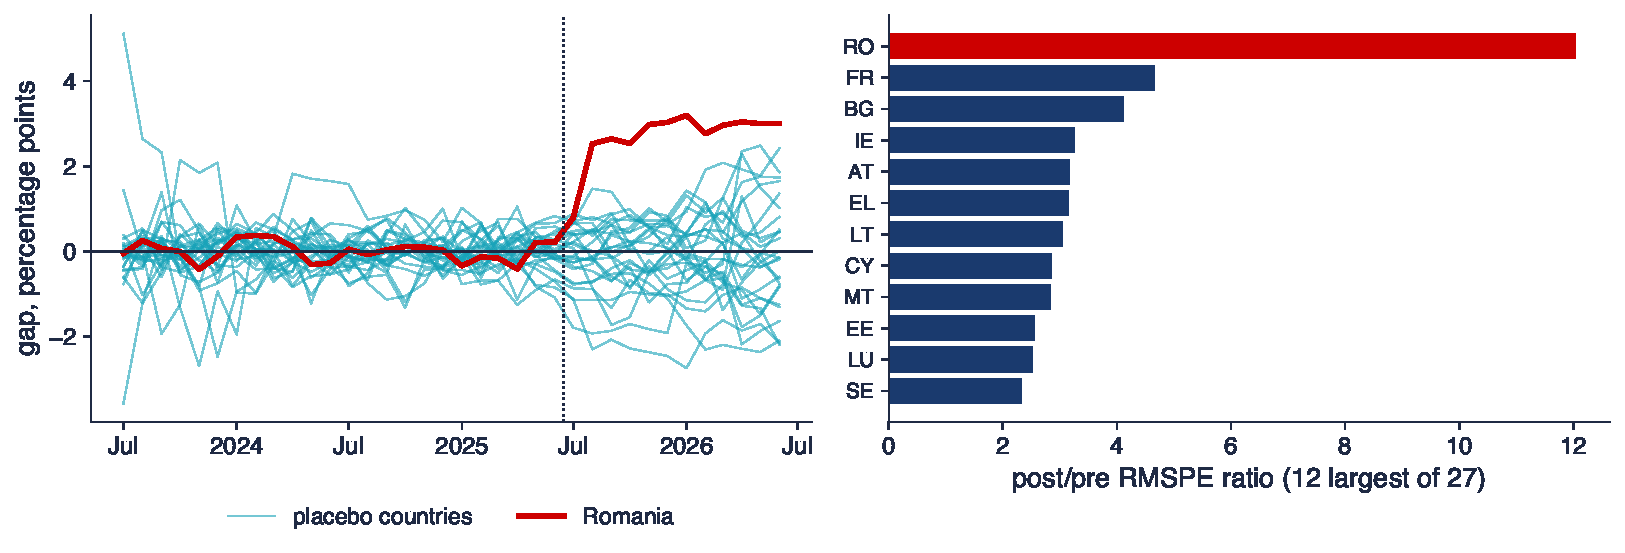
\includegraphics[width=0.97\textwidth,height=0.56\textheight,keepaspectratio]{ats_ch14_ro_placebo.pdf}
\end{center}
\vspace{-0.25cm}
\begin{itemize}
    \item Demeaned SC applied to every EU country in turn; left: gaps; right: the 12 largest post/pre RMSPE ratios over July 2025 -- June 2026
\end{itemize}
\quantlet{ATS\_ch14\_romania}{\qlurl{ATS_ch14_romania}}
\end{frame}

\begin{frame}{Interpreting the Romanian placebos}
\itemsize{\small}
\begin{itemize}
    \item Romania has the largest ratio (12.0; next France, 4.7): $p = 1/27$ = 0.037
    \item No placebo country shows a jump of this size in July--August 2025: the effect is not a common European shock
    \item The permutation p-value treats Romania as one of 27 exchangeable units; it is a measure of rarity, not a sampling-based confidence statement
    \item Other countries' measures in the window (tax changes, the end of their own caps) bias the effect towards zero if they raised inflation there
\end{itemize}
\end{frame}

\begin{frame}{How much was the tax?}
\itemsize{\footnotesize}
\begin{center}
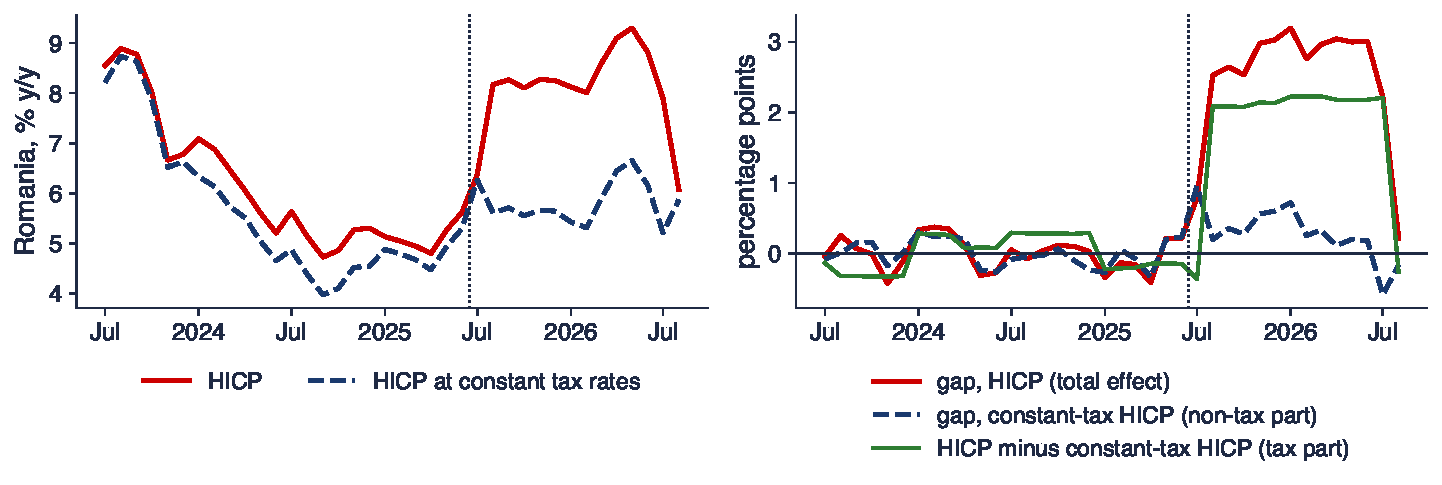
\includegraphics[width=0.97\textwidth,height=0.54\textheight,keepaspectratio]{ats_ch14_ro_tax.pdf}
\end{center}
\vspace{-0.25cm}
\begin{itemize}
    \item Left: Romanian HICP and HICP at constant tax rates (\refEuroCT); right: the total gap, the gap of the constant-tax inflation (same demeaned SC on all countries) and the tax wedge
\end{itemize}
\quantlet{ATS\_ch14\_romania}{\qlurl{ATS_ch14_romania}}
\end{frame}

\begin{frame}{Interpreting the tax decomposition}
\itemsize{\small}
\begin{itemize}
    \item The constant-tax index assumes full and immediate pass-through of tax changes: the tax wedge jumps by 2.09 pp in August 2025, when the VAT rose
    \item Average over twelve months: total 2.70 pp = tax wedge 1.95 pp + constant-tax gap 0.40 pp: about 72\% of the effect is mechanical tax
    \item The non-tax part peaks in July 2025 (0.96 pp): the end of the electricity cap, which is a price, not a tax
    \item Pass-through of VAT to consumer prices is often incomplete and asymmetric \refBMKW; the constant-tax index is an accounting benchmark, not a measured pass-through
\end{itemize}
\end{frame}

\begin{frame}{Staggered adoption and two-way fixed effects (1/2)}
\itemsize{\small}
\begin{itemize}
    \item Many units adopt at different dates $g$ (their cohort); the static TWFE regression \[ Y_{it} = \alpha_i + \beta_t + \tau D_{it} + u_{it} \]
    \begin{itemize}
        \item $D_{it} = 1$ if unit $i$ is treated at $t$; $\alpha_i$, $\beta_t$: unit and period fixed effects; $\tau$: a single treatment effect
    \end{itemize}
    \item \refGB: $\hat\tau$ is a weighted average of all 2$\times$2 DiDs
    \begin{itemize}
        \item including ``forbidden'' ones that use already-treated units as controls
        \item with effects that grow over time some weights are negative \refdCDH: $\hat\tau$ can even have the wrong sign
    \end{itemize}
\end{itemize}
\end{frame}

\begin{frame}{Staggered adoption and two-way fixed effects (2/2)}
\itemsize{\small}
\begin{itemize}
    \item \refCSA: group-time effects, each compared only with never-treated units \[ ATT(g, t) = \E[Y_t - Y_{g-1}\mid G = g] - \E[Y_t - Y_{g-1}\mid \text{never treated}] \]
    \begin{itemize}
        \item $G$: the adoption date of a unit; $Y_{g-1}$: the outcome in the last period before adoption; $ATT$: average treatment effect on the treated
        \item then aggregate by exposure ($t - g$) or by cohort
    \end{itemize}
    \item Related: interaction-weighted event studies \refSA; a guide to the new DiD literature \refRSBP
    \item Pre-trend tests have low power; report the sensitivity of the effect to violations of parallel trends
\end{itemize}
\end{frame}

\begin{frame}{TWFE against Callaway and Sant'Anna}
\itemsize{\footnotesize}
\begin{center}
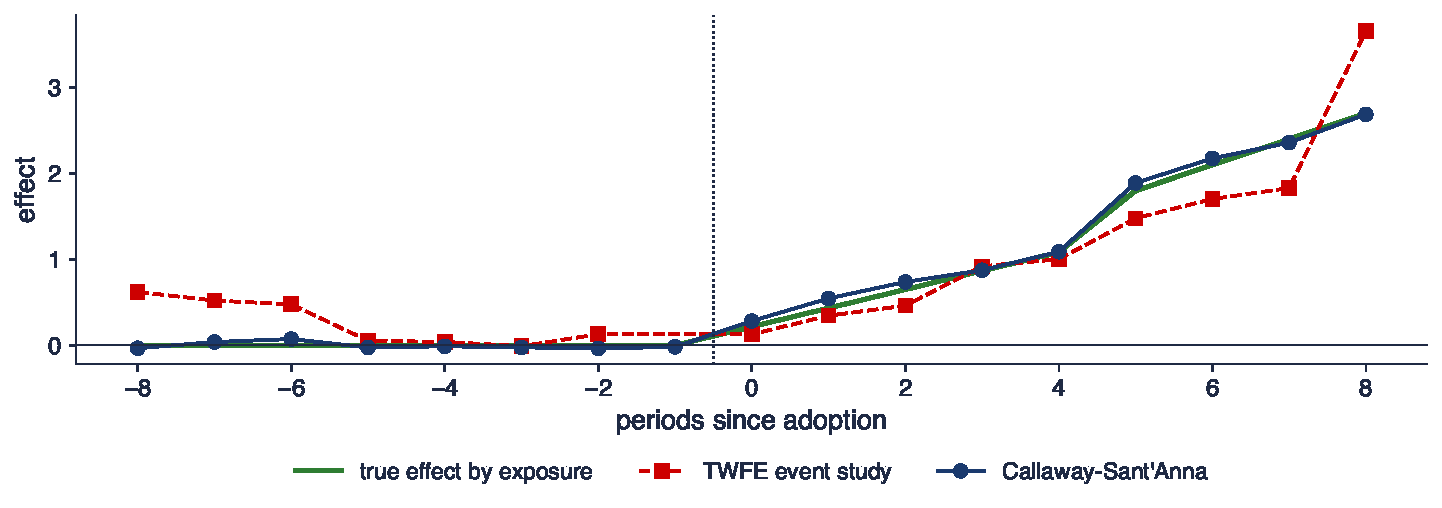
\includegraphics[width=0.97\textwidth,height=0.56\textheight,keepaspectratio]{ats_ch14_staggered.pdf}
\end{center}
\vspace{-0.25cm}
\begin{itemize}
    \item Simulated panel: three cohorts adopting in periods 6, 11 and 16 and a never-treated group; effects grow with exposure, faster for early adopters
\end{itemize}
\quantlet{ATS\_ch14\_did\_dml}{\qlurl{ATS_ch14_did_dml}}
\end{frame}

\begin{frame}{Interpreting staggered adoption}
\itemsize{\small}
\begin{itemize}
    \item Static TWFE: 0.55; true average effect on the treated: 1.99; Callaway--Sant'Anna: 2.04
    \item TWFE uses early adopters as controls for late adopters while their effect is still growing: those comparisons subtract part of the effect
    \item The TWFE event study is distorted at long exposures (binned endpoint 3.66 against 2.70); CS gives 2.69
    \item With one treated country (Romania) there is no staggering; with EU-wide policies adopted at different dates, there is
\end{itemize}
\end{frame}

\begin{frame}{Recap: Beyond synthetic control}
\itemsize{\small}
\begin{itemize}
    \item An intercept fixes level differences; ridge augmentation corrects the remaining imbalance; SDID combines unit and time weights
    \item Romania 2025: 2.7--2.8 pp more annual inflation for twelve months, most of it the mechanical VAT effect, and a falsification that holds
    \item Staggered adoption breaks TWFE; use group-time estimators
\end{itemize}
\end{frame}


%=============================================================================
\section{Bayesian structural time series and CausalImpact}
%=============================================================================

\begin{frame}{The CausalImpact model (1/2)}
\itemsize{\small}
\begin{itemize}
    \item \refCI: the outcome is a trend plus a seasonal component plus a regression on control series \[ y_t = \mu_t + \gamma_t + \beta'x_t + \varepsilon_t, \qquad \mu_{t+1} = \mu_t + \delta_t + \eta_t, \qquad \delta_{t+1} = \delta_t + \zeta_t \]
    \begin{itemize}
        \item $\mu_t$: local level; $\delta_t$: local slope; $\gamma_t$: seasonal component; $x_t$: control series with coefficients $\beta$; $\varepsilon_t, \eta_t, \zeta_t$: independent Normal noises
    \end{itemize}
    \item A structural time series model \refHar{} in state space form, filtered and smoothed by Kalman (\atschlink{https://danpele.github.io/Advanced-Time-Series/EN/Courses/chapter6_state_space_models_bayesian_filtering.pdf}{Chapter 6}, \refDK)
    \begin{itemize}
        \item a spike-and-slab prior on $\beta$ selects the controls \refSV; the posterior is computed by MCMC
    \end{itemize}
\end{itemize}
\end{frame}

\begin{frame}{The CausalImpact model (2/2)}
\itemsize{\small}
\begin{itemize}
    \item Fit on the pre-period; simulate the post-period counterfactual $y^{(s)}_t(0)$ from the posterior predictive, given the observed $x_t$
    \begin{itemize}
        \item $s$: the index of a simulated path; effects $y_t - y^{(s)}_t(0)$, pointwise and cumulative
        \item credible intervals from the quantiles of the simulated effects
    \end{itemize}
    \item \textbf{Identification}
    \begin{itemize}
        \item the controls are \textbf{not affected} by the treatment
        \item their relation with $y$ is stable after $T_0$
    \end{itemize}
\end{itemize}
\end{frame}

\begin{frame}{Our implementation}
\itemsize{\small}
\begin{itemize}
    \item \texttt{statsmodels} \texttt{UnobservedComponents}: local level + regression on the controls, maximum likelihood on the pre-period
    \begin{itemize}
        \item 1000 counterfactual paths: parameters drawn from their asymptotic normal distribution, then the state simulated forward from the end of the pre-period given the observed controls
    \end{itemize}
    \item Differences from the R package: no spike-and-slab selection, no MCMC; parameter uncertainty by a Gaussian approximation
    \begin{itemize}
        \item the transparent version keeps every step visible; with few controls the two give similar intervals
    \end{itemize}
    \item Outputs: average effect with a 95\% interval, cumulative effect, and the tail probability that the counterfactual mean exceeds the observed one
\end{itemize}
\end{frame}

\begin{frame}{Case study: the US spot Bitcoin ETFs}
\itemsize{\small}
\begin{columns}[T]
\begin{column}{0.34\textwidth}
\centering

\includegraphics[height=0.40\textheight]{ch14_bitcoin_atm_2016.jpg}\\[1mm]
\imgcap{A Bitcoin ATM, Prague}
\imgcredit{https://commons.wikimedia.org/wiki/File:Bitcoin_ATM_Prague.jpg}{Photo: Perituss (2016); CC0; Wikimedia Commons}
\end{column}
\begin{column}{0.64\textwidth}
\begin{itemize}
    \item \textbf{10 January 2024} \refSEC
    \begin{itemize}
        \item the SEC approves eleven spot Bitcoin ETPs (exchange-traded products); trading starts on 11 January
    \end{itemize}
    \item Question
    \begin{itemize}
        \item did the approval change Bitcoin volatility (institutional demand, arbitrage between spot and ETF)?
    \end{itemize}
    \item Design
    \begin{itemize}
        \item outcome: weekly log realised variance of Bitcoin
        \item controls: the same measure for the S\&P 500, Nasdaq 100, gold and EUR/USD
        \item pre-period January 2023 -- 7 January 2024 (53 weeks); post: 25 weeks to June 2024
    \end{itemize}
    \item Anticipation (dotted lines)
    \begin{itemize}
        \item BlackRock filed on 15 June 2023; a court ruled for Grayscale on 29 August 2023
    \end{itemize}
\end{itemize}
\end{column}
\end{columns}
\end{frame}

\begin{frame}{CausalImpact for the spot ETF approval}
\itemsize{\footnotesize}
\begin{center}
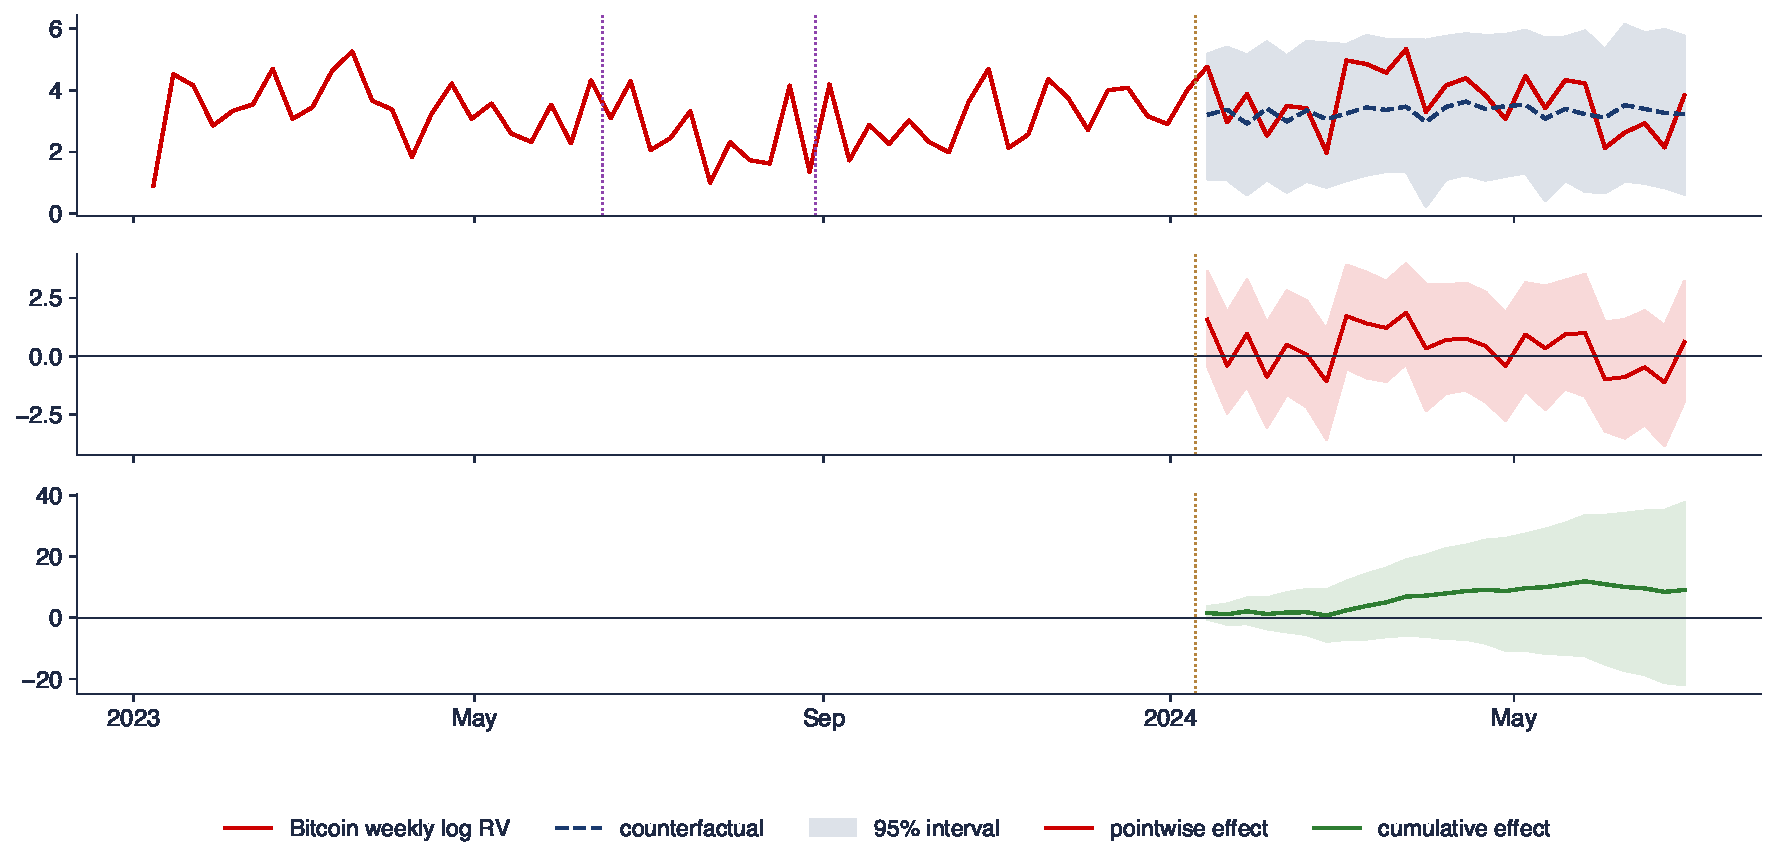
\includegraphics[width=0.97\textwidth,height=0.6\textheight,keepaspectratio]{ats_ch14_btc.pdf}
\end{center}
\vspace{-0.25cm}
\begin{itemize}
    \item Top: observed and counterfactual log RV with a 95\% interval; middle: pointwise effect; bottom: cumulative effect
\end{itemize}
\quantlet{ATS\_ch14\_causalimpact}{\qlurl{ATS_ch14_causalimpact}}
\end{frame}

\begin{frame}{Interpreting the ETF analysis}
\itemsize{\small}
\begin{itemize}
    \item Average effect on weekly log RV: 0.36 (95\% interval [\ensuremath{-}0.87, 1.50]), tail probability 0.26: no detectable change
    \item The level variance is small (0.011) against the irregular one (0.94): weekly crypto volatility is mostly noise, and the controls explain little
    \item The finding agrees with a peer-reviewed study: no effect on Bitcoin's own volatility \refBBG
    \item Absence of evidence is not evidence of absence: with this noise, a 50\% change in volatility would not be detected
\end{itemize}
\end{frame}

\begin{frame}{Placebo dates and the choice of controls}
\itemsize{\footnotesize}
\begin{center}
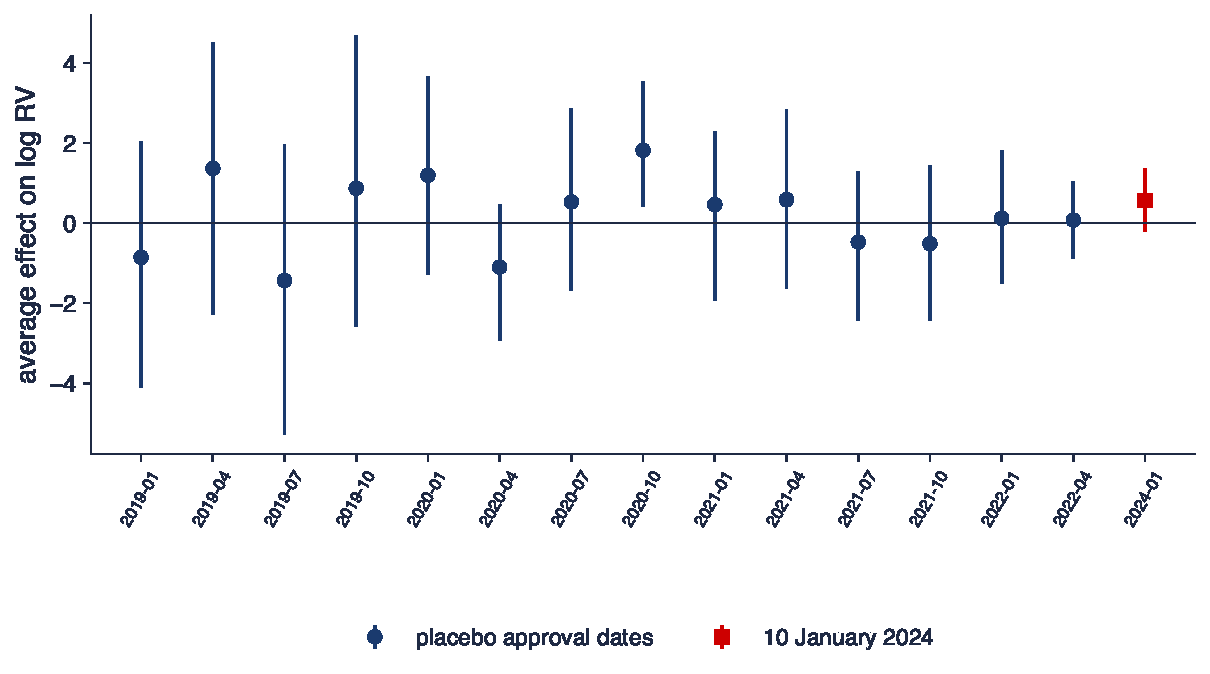
\includegraphics[width=0.97\textwidth,height=0.54\textheight,keepaspectratio]{ats_ch14_btc_placebo.pdf}
\end{center}
\vspace{-0.25cm}
\begin{itemize}
    \item The same analysis with 14 fictitious approval dates in 2019--2022 (53 pre-weeks, 25 post-weeks each) and the true date with the same window lengths
\end{itemize}
\quantlet{ATS\_ch14\_causalimpact}{\qlurl{ATS_ch14_causalimpact}}
\end{frame}

\begin{frame}{Interpreting the placebo dates}
\itemsize{\small}
\begin{itemize}
    \item Only 1 of the 14 placebo intervals excludes zero; the placebo estimates have a standard deviation of 0.97: the real estimate is inside their range
    \item With Ether as an extra control: 0.18 [\ensuremath{-}0.47, 0.87]; but Ether may itself respond to the approval: a treated control biases the effect towards zero
    \item Moving $T_0$ back to the BlackRock filing (June 2023): \ensuremath{-}0.02 [\ensuremath{-}1.74, 1.62]: still nothing, so anticipation does not hide a large effect
    \item Placebo dates calibrate the credible intervals: if many placebos look ``significant'', the model is misspecified
\end{itemize}
\end{frame}

\begin{frame}{Recap: BSTS and CausalImpact}
\itemsize{\small}
\begin{itemize}
    \item A state space forecast of the untreated path from control series; uncertainty from parameters and states
    \item Its key assumption is about the controls: unaffected and stably related; check with placebo dates
    \item The spot ETF approval did not change Bitcoin volatility detectably; the design could not see small effects
\end{itemize}
\end{frame}


%=============================================================================
\section{Double machine learning and honest identification}
%=============================================================================

\begin{frame}{Double/debiased machine learning for time series (1/2)}
\itemsize{\small}
\begin{itemize}
    \item \refDML: the \textbf{partially linear model} \[ y_t = \theta d_t + g(X_t) + u_t, \qquad d_t = m(X_t) + v_t \]
    \begin{itemize}
        \item $d_t$: the treatment; $\theta$: its effect; $X_t$: control variables; $g$, $m$: unknown \textbf{nuisance functions}, learned by machine learning; $u_t, v_t$: errors
    \end{itemize}
    \item \textbf{Orthogonal score}: regress the residual of $y$ on the residual of $d$ \[ \psi = \big(y_t - \ell(X_t) - \theta(d_t - m(X_t))\big)\big(d_t - m(X_t)\big), \qquad \ell(X) = \E[y\mid X] \]
    \begin{itemize}
        \item $\hat\theta$ solves $\frac1T\sum_t\psi_t = 0$; first-order insensitive to errors in $\ell$ and $m$
    \end{itemize}
\end{itemize}
\end{frame}

\begin{frame}{Double/debiased machine learning for time series (2/2)}
\itemsize{\small}
\begin{itemize}
    \item \textbf{Cross-fitting}: the nuisance functions are fitted on other folds than the one where $\psi$ is evaluated
    \begin{itemize}
        \item for time series use \textbf{contiguous blocks} with a gap around the held-out block
        \item standard error from a HAC variance of $\psi$
    \end{itemize}
    \item DML removes regularisation and overfitting bias; it does not create identification
    \begin{itemize}
        \item $d_t$ must be unconfounded given $X_t$
    \end{itemize}
\end{itemize}
\end{frame}

\begin{frame}{DML against a linear adjustment}
\itemsize{\footnotesize}
\begin{center}
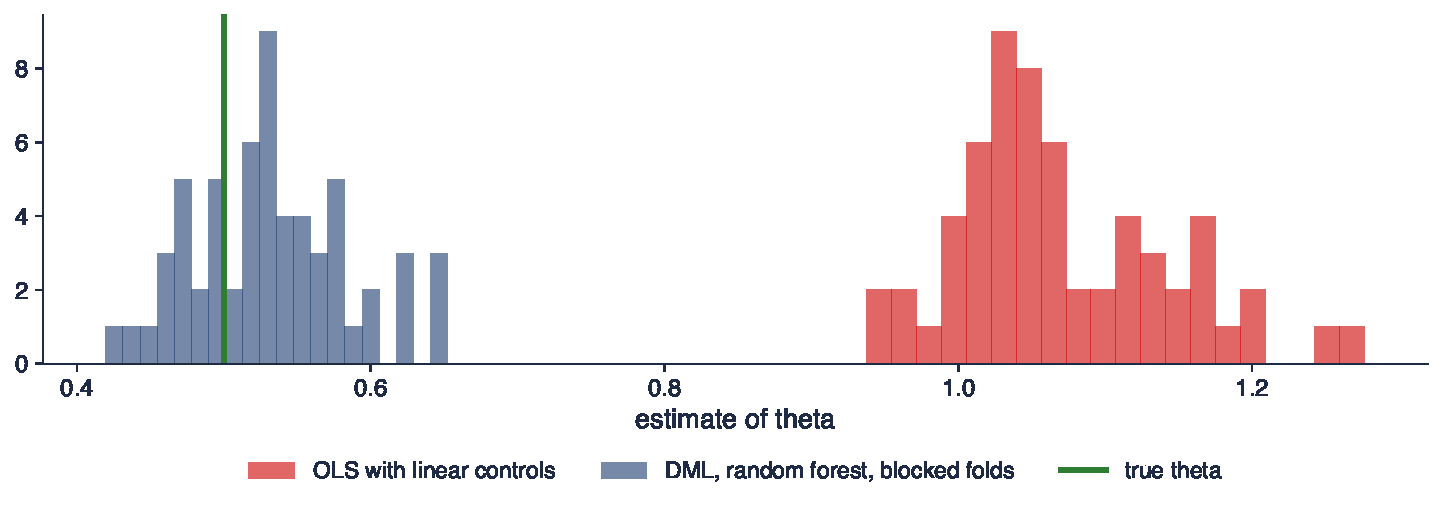
\includegraphics[width=0.97\textwidth,height=0.54\textheight,keepaspectratio]{ats_ch14_dml.pdf}
\end{center}
\vspace{-0.25cm}
\begin{itemize}
    \item Simulated dependent data: 10 VAR(1) covariates, nonlinear $g$ and $m$, AR(1) errors, $\theta = 0.5$, $T = 1\,000$, 60 replications; random forests with five blocked folds
\end{itemize}
\quantlet{ATS\_ch14\_did\_dml}{\qlurl{ATS_ch14_did_dml}}
\end{frame}

\begin{frame}{Interpreting the DML experiment}
\itemsize{\small}
\begin{itemize}
    \item OLS with linear controls: mean estimate 1.07, far from 0.5: the nonlinear confounding is not removed
    \item DML: mean 0.53, standard deviation 0.05; 95\% HAC intervals cover the true value in 88\% of the replications
    \item The remaining bias comes from the forests' errors on a finite sample; it shrinks with $T$
    \item In macro time series the treatment is rarely unconfounded given observables: DML is a tool for the estimation step, after identification is argued
\end{itemize}
\end{frame}

\begin{frame}{Identification, method by method}
\itemsize{\small}
\begin{center}
\scriptsize
\begin{tabular}{>{\raggedright\arraybackslash}p{2.6cm}>{\raggedright\arraybackslash}p{5.4cm}>{\raggedright\arraybackslash}p{4.4cm}}
\toprule
\textbf{Method} & \textbf{Key assumption} & \textbf{Check} \\
\midrule
Granger, PCMCI & no hidden common causes; correct timing; faithfulness & add candidate confounders; change the frequency \\
ITS, event study & nothing else changes at $T_0$; no anticipation & placebo dates; news timeline \\
Synthetic control, SDID & factor model; donors unaffected; treated unit in the donors' range & pre-fit, placebos, leave-one-out \\
DiD (staggered) & parallel trends; no anticipation & pre-trends with sensitivity analysis \\
CausalImpact & controls unaffected; stable relation & placebo dates; alternative control sets \\
SVAR, LP, DML & as good as random given the past or an instrument & narrative evidence; instrument strength \\
\bottomrule
\end{tabular}
\end{center}
\end{frame}

\begin{frame}{Honest reporting}
\itemsize{\small}
\begin{itemize}
    \item State the estimand (which effect, on which unit, over which horizon) before choosing the method
    \item Fix treatment dates, windows, donors and estimators before looking at post-treatment data; publish the pre-registration
    \item Report every placebo, every specification and every deviation from the published design; a specification curve shows them together
    \item Separate statistical uncertainty (intervals) from identification uncertainty (assumptions); the second is usually larger
    \item Read \refAI{} and \refAba{} before writing a policy evaluation
\end{itemize}
\end{frame}


%=============================================================================
\section{AI for scientific discovery}
%=============================================================================

\begin{frame}{An open question}
\itemsize{\small}
\begin{itemize}
    \item The question
    \begin{itemize}
        \item how much of Romania's 2025--2026 inflation surge was caused by the end of the electricity cap and the VAT increase?
        \item how robust is the answer to the choice of method?
    \end{itemize}
    \item A testable form
    \begin{itemize}
        \item formal: $H_0$: the average gap over July 2025 -- June 2026 is zero; the claim ``between 2 and 3.5 pp'' must hold for every pre-registered estimator with a good pre-fit
        \item falsified if a reasonable specification gives less than 2 pp or a placebo country matches Romania
    \end{itemize}
    \item Why it matters
    \begin{itemize}
        \item monetary policy must tell one-off price-level effects from persistent inflation
        \item second-round effects decide interest rates
        \item literature to start from: \refADHb, \refASCM, \refSDID, \refBMKW
    \end{itemize}
\end{itemize}
\end{frame}

\begin{frame}{The discovery loop with an AI assistant}
\itemsize{\footnotesize}
\begin{itemize}
    \item An AI assistant (an LLM such as Claude, ChatGPT, Gemini or Copilot) speeds up each step; Semantic Scholar and Elicit help with the literature
    \begin{itemize}
        \item \textbf{literature}: \aiprompt{List peer-reviewed studies since 2015 that estimate VAT pass-through to consumer prices with synthetic control or DiD; give DOIs and the estimated pass-through.} Then check every DOI on Crossref
        \item \textbf{design}: \aiprompt{Write a pre-registration: outcome, donors, exclusions, pre-period, estimators, placebo tests, what counts as a robust effect.}
        \item \textbf{code and replication}: reproduce first the German weights (Austria 0.42; USA 0.22; ...) before running anything on Romania
        \item \textbf{critique}: \aiprompt{Act as a hostile referee: which EU countries had their own energy or tax measures in 2025--2026, and how would each bias the estimate?}
    \end{itemize}
    \item Report: what was asked, what was kept, what was rejected (AI\_USE.md, AI\_ERRORS.md)
\end{itemize}
\end{frame}

\begin{frame}{What the human checks}
\itemsize{\small}
\begin{itemize}
    \item Every reference exists and says what is claimed (DOI resolves, title matches, the result is in the paper)
    \item Policy dates are taken from official sources (Monitorul Oficial, Eurostat, SEC), not from the assistant's memory
    \item The donor pool excludes countries with their own large shocks in the window, and the exclusions are written before the results are seen
    \item Placebo tests are run with exactly the same code and settings as the main estimate
    \item An AI claim that ``the synthetic control proves the VAT caused 3 pp of inflation'' is rewritten as an estimate with assumptions
\end{itemize}
\end{frame}

\begin{frame}{Mini-case: a specification curve for Romania}
\itemsize{\footnotesize}
\begin{center}
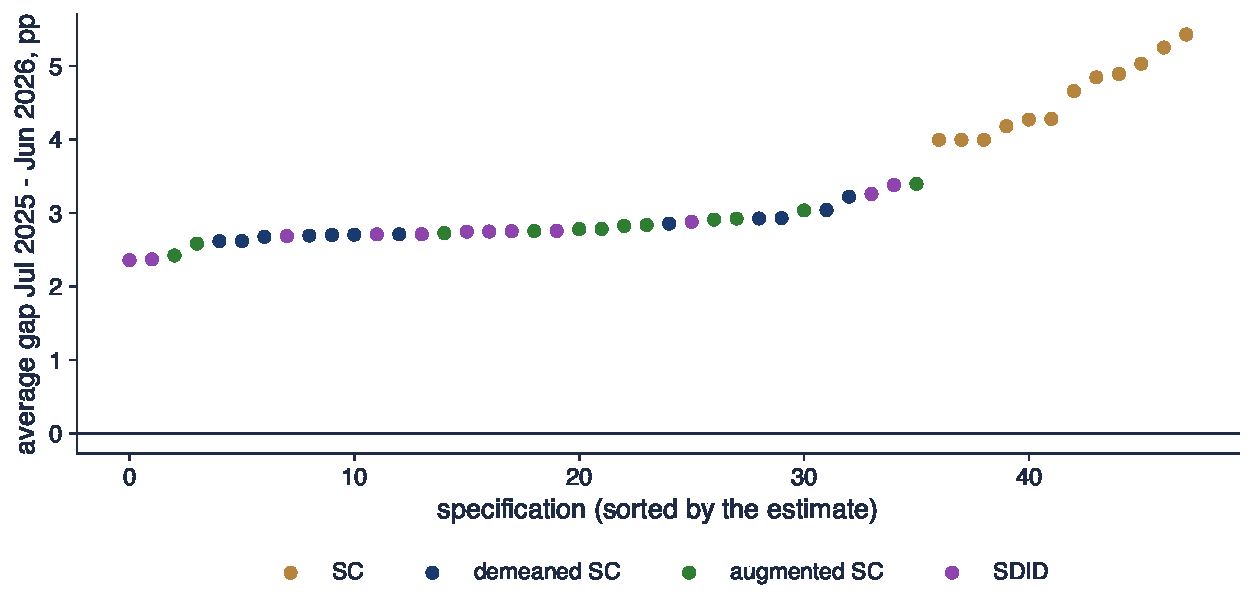
\includegraphics[width=0.97\textwidth,height=0.54\textheight,keepaspectratio]{ats_ch14_ai_case.pdf}
\end{center}
\vspace{-0.25cm}
\begin{itemize}
    \item 48 specifications: four estimators $\times$ three donor pools (EU-26, euro area, non-euro EU) $\times$ four pre-periods (from 2017, 2019, July 2023, 2024; the 2021--2023 surge excluded)
    \item Without classic SC: from 2.36 to 3.40 pp, median 2.75; classic SC: median 4.47 (poor pre-fit); 0 specifications give a non-positive effect: the hypothesis survives
\end{itemize}
\quantlet{ATS\_ch14\_ai\_case}{\qlurl{ATS_ch14_ai_case}}
\end{frame}

\begin{frame}{Project idea}
\itemsize{\small}
\begin{itemize}
    \item \textbf{Tax pass-through in Central and Eastern Europe with synthetic controls}: replicate first, then extend
    \begin{itemize}
        \item replicate: \refADHb{} (Table 1, Figures 2--5) with the public data, then this chapter's Romanian estimate
        \item extend: product-level HICP (food, energy, services) to measure pass-through by VAT rate
        \item other episodes (Hungary 2012, Croatia 2023 euro adoption); conformal intervals \refCWZ
        \item pre-register: donors and exclusions, windows, estimators, placebos, the robustness rule
    \end{itemize}
    \item Deliverables follow the course rules: repository, report, AI\_USE.md, AI\_ERRORS.md, oral defence
\end{itemize}
\end{frame}


%=============================================================================
\section{Wrap-up}
%=============================================================================

\begin{frame}{Key takeaways}
\itemsize{\small}
\begin{itemize}
    \item Granger causality and its relatives (TE, PCMCI, CCM) describe predictive structure; causal claims need assumptions about the assignment
    \item Interrupted series and event studies use the unit's own past; dependence enlarges their standard errors
    \item Synthetic control and its successors use other units; placebos are the inference, a long pre-fit is the justification
    \item Replication exposes fragility: German reunification holds, the Brexit gap depends on data vintage
    \item Romania 2025: a robust 2.7--2.8 pp twelve-month effect, mostly mechanical VAT; Bitcoin ETFs: no detectable effect on volatility
\end{itemize}
\end{frame}

\begin{frame}{Self-assessment}
\itemsize{\small}
\begin{columns}[T]
\begin{column}{0.58\textwidth}
\begin{block}{Questions}
\begin{itemize}
    \item Why can adding a variable to the information set remove a Granger causality?
    \item What does conditioning on the parents of the source achieve in the MCI test?
    \item Why does classic synthetic control fail for Romanian inflation?
    \item What is the smallest placebo p-value with 23 donors?
    \item Why can a static TWFE estimate have the wrong sign under staggered adoption?
\end{itemize}
\end{block}
\end{column}
\begin{column}{0.38\textwidth}
\begin{block}{Next: \atschlink{https://danpele.github.io/Advanced-Time-Series/EN/Courses/chapter15_review_project_defence.pdf}{Chapter 15}}
\begin{itemize}
    \item Review and project defence
    \item one synthesis per chapter; the replication project and the oral defence
\end{itemize}
\end{block}
\end{column}
\end{columns}
\end{frame}


%=============================================================================
\section{Appendix}
%=============================================================================

\begin{frame}{Appendix: the bias bound of synthetic control}
\hypertarget{atsapp1}{}\atsappback{atssrc2}{Back}
\itemsize{\small}
\begin{itemize}
    \item Factor model $Y_{jt}(0) = \delta_t + \lambda_t\mu_j + \varepsilon_{jt}$ ($F$ factors); weights with $\sum_jw_jY_{jt} = Y_{1t}$, $t \le T_0$
    \item Stack the pre-period: $\lambda^P(\mu_1 - \sum_jw_j\mu_j) = -(\varepsilon^P_1 - \sum_jw_j\varepsilon^P_j)$; if $\lambda^{P\prime}\lambda^P$ is invertible, solve for the loading imbalance
    \item Then $Y_{1t}(0) - \sum_jw_jY_{jt} = \lambda_t(\lambda^{P\prime}\lambda^P)^{-1}\lambda^{P\prime}\sum_jw_j\varepsilon^P_j - \dots + (\varepsilon_{1t} - \sum_jw_j\varepsilon_{jt})$
    \item The first term has mean zero only approximately (the weights depend on the $\varepsilon^P$); ADH (2010, Appendix B) bound it by a quantity of order $J^{1/p}\bar m_p^{1/p}F\,\bar\lambda^2/(\xi T_0^{1 - 1/p})$: small when $T_0$ is large relative to $J$
\end{itemize}
\end{frame}

\begin{frame}{Appendix: Gaussian transfer entropy equals half the Geweke measure}
\hypertarget{atsapp2}{}\atsappback{atssrc1}{Back}
\itemsize{\small}
\begin{itemize}
    \item For jointly Gaussian variables $I(Y; X\mid Z) = \frac12\ln\dfrac{\mathrm{Var}(Y\mid Z)}{\mathrm{Var}(Y\mid X, Z)}$ (the entropy of a Gaussian is $\frac12\ln(2\pi e\sigma^2)$)
    \item With $Y = y_t$, $X = x^{(l)}_{t-1}$, $Z = y^{(k)}_{t-1}$, the conditional variances are the residual variances of the restricted and full Granger regressions
    \item Hence $TE_{x\to y} = \frac12F_{x\to y}$, and $2T\cdot\widehat{TE} \approx T\hat F \approx W$, the likelihood-ratio form of the Granger Wald test \refBBS
    \item Non-Gaussian data break the equality: TE then detects dependence that a linear test misses (Section 1)
\end{itemize}
\end{frame}


%=============================================================================
\section{References}
%=============================================================================

\begin{frame}{References (1/5)}
\itemsize{\tiny}
\begin{itemize}
    \item Abadie, A., Diamond, A., \& Hainmueller, J. (2015). Comparative politics and the synthetic control method. \textit{American Journal of Political Science}, 59(2), 495--510. \href{https://doi.org/10.1111/ajps.12116}{doi:10.1111/ajps.12116}
    \item Abadie, A., Diamond, A., \& Hainmueller, J. (2014). Replication data for: Comparative politics and the synthetic control method. Harvard Dataverse, version 2.1 (CC0); erratum and updated archive, version 3 (2026). \href{https://doi.org/10.7910/DVN/24714}{doi:10.7910/DVN/24714}
    \item Abadie, A., Diamond, A., \& Hainmueller, J. (2011). Synth: An R package for synthetic control methods in comparative case studies. \textit{Journal of Statistical Software}, 42(13), 1--17. \href{https://doi.org/10.18637/jss.v042.i13}{doi:10.18637/jss.v042.i13}
    \item Abadie, A., Diamond, A., \& Hainmueller, J. (2010). Synthetic control methods for comparative case studies: Estimating the effect of California’s tobacco control program. \textit{Journal of the American Statistical Association}, 105(490), 493--505. \href{https://doi.org/10.1198/jasa.2009.ap08746}{doi:10.1198/jasa.2009.ap08746}
    \item Abadie, A., \& Gardeazabal, J. (2003). The economic costs of conflict: A case study of the Basque Country. \textit{American Economic Review}, 93(1), 113--132. \href{https://doi.org/10.1257/000282803321455188}{doi:10.1257/000282803321455188}
    \item Abadie, A. (2021). Using synthetic controls: Feasibility, data requirements, and methodological aspects. \textit{Journal of Economic Literature}, 59(2), 391--425. \href{https://doi.org/10.1257/jel.20191450}{doi:10.1257/jel.20191450}
    \item Andrews, D. W. K. (2003). End-of-sample instability tests. \textit{Econometrica}, 71(6), 1661--1694. \href{https://doi.org/10.1111/1468-0262.00466}{doi:10.1111/1468-0262.00466}
    \item Angrist, J. D., Jordà, Ò., \& Kuersteiner, G. M. (2018). Semiparametric estimates of monetary policy effects: String theory revisited. \textit{Journal of Business \& Economic Statistics}, 36(3), 371--387. \href{https://doi.org/10.1080/07350015.2016.1204919}{doi:10.1080/07350015.2016.1204919}
    \item Arkhangelsky, D., Athey, S., Hirshberg, D. A., Imbens, G. W., \& Wager, S. (2021). Synthetic difference-in-differences. \textit{American Economic Review}, 111(12), 4088--4118. \href{https://doi.org/10.1257/aer.20190159}{doi:10.1257/aer.20190159}
    \item Athey, S., \& Imbens, G. W. (2017). The state of applied econometrics: Causality and policy evaluation. \textit{Journal of Economic Perspectives}, 31(2), 3--32. \href{https://doi.org/10.1257/jep.31.2.3}{doi:10.1257/jep.31.2.3}
    \item Babalos, V., Bouri, E., \& Gupta, R. (2025). Does the introduction of US spot Bitcoin ETFs affect spot returns and volatility of major cryptocurrencies? \textit{The Quarterly Review of Economics and Finance}, 102, 102006. \href{https://doi.org/10.1016/j.qref.2025.102006}{doi:10.1016/j.qref.2025.102006}
    \item Bai, J. (2009). Panel data models with interactive fixed effects. \textit{Econometrica}, 77(4), 1229--1279. \href{https://doi.org/10.3982/ECTA6135}{doi:10.3982/ECTA6135}
    \item Barnett, L., Barrett, A. B., \& Seth, A. K. (2009). Granger causality and transfer entropy are equivalent for Gaussian variables. \textit{Physical Review Letters}, 103(23), 238701. \href{https://doi.org/10.1103/PhysRevLett.103.238701}{doi:10.1103/PhysRevLett.103.238701}
    \item Baskerville, E. B., \& Cobey, S. (2017). Does influenza drive absolute humidity? \textit{Proceedings of the National Academy of Sciences}, 114(12), E2270--E2271. \href{https://doi.org/10.1073/pnas.1700369114}{doi:10.1073/pnas.1700369114}
\end{itemize}
\end{frame}

\begin{frame}{References (2/5)}
\itemsize{\tiny}
\begin{itemize}
    \item Benedek, D., De Mooij, R. A., Keen, M., \& Wingender, P. (2020). Varieties of VAT pass through. \textit{International Tax and Public Finance}, 27(4), 890--930. \href{https://doi.org/10.1007/s10797-019-09566-5}{doi:10.1007/s10797-019-09566-5}
    \item Ben-Michael, E., Feller, A., \& Rothstein, J. (2021). The augmented synthetic control method. \textit{Journal of the American Statistical Association}, 116(536), 1789--1803. \href{https://doi.org/10.1080/01621459.2021.1929245}{doi:10.1080/01621459.2021.1929245}
    \item Bojinov, I., \& Shephard, N. (2019). Time series experiments and causal estimands: Exact randomization tests and trading. \textit{Journal of the American Statistical Association}, 114(528), 1665--1682. \href{https://doi.org/10.1080/01621459.2018.1527225}{doi:10.1080/01621459.2018.1527225}
    \item Born, B., Müller, G. J., Schularick, M., \& Sedláček, P. (2019). The costs of economic nationalism: Evidence from the Brexit experiment. \textit{The Economic Journal}, 129(623), 2722--2744. \href{https://doi.org/10.1093/ej/uez020}{doi:10.1093/ej/uez020}
    \item Breitung, J., \& Candelon, B. (2006). Testing for short- and long-run causality: A frequency-domain approach. \textit{Journal of Econometrics}, 132(2), 363--378. \href{https://doi.org/10.1016/j.jeconom.2005.02.004}{doi:10.1016/j.jeconom.2005.02.004}
    \item Brodersen, K. H., Gallusser, F., Koehler, J., Remy, N., \& Scott, S. L. (2015). Inferring causal impact using Bayesian structural time-series models. \textit{The Annals of Applied Statistics}, 9(1), 247--274. \href{https://doi.org/10.1214/14-AOAS788}{doi:10.1214/14-AOAS788}
    \item Callaway, B., \& Sant’Anna, P. H. C. (2021). Difference-in-differences with multiple time periods. \textit{Journal of Econometrics}, 225(2), 200--230. \href{https://doi.org/10.1016/j.jeconom.2020.12.001}{doi:10.1016/j.jeconom.2020.12.001}
    \item Chernozhukov, V., Chetverikov, D., Demirer, M., Duflo, E., Hansen, C., Newey, W., \& Robins, J. (2018). Double/debiased machine learning for treatment and structural parameters. \textit{The Econometrics Journal}, 21(1), C1--C68. \href{https://doi.org/10.1111/ectj.12097}{doi:10.1111/ectj.12097}
    \item Chernozhukov, V., Wüthrich, K., \& Zhu, Y. (2021). An exact and robust conformal inference method for counterfactual and synthetic controls. \textit{Journal of the American Statistical Association}, 116(536), 1849--1864. \href{https://doi.org/10.1080/01621459.2021.1920957}{doi:10.1080/01621459.2021.1920957}
    \item de Chaisemartin, C., \& D’Haultfœuille, X. (2020). Two-way fixed effects estimators with heterogeneous treatment effects. \textit{American Economic Review}, 110(9), 2964--2996. \href{https://doi.org/10.1257/aer.20181169}{doi:10.1257/aer.20181169}
    \item Doudchenko, N., \& Imbens, G. W. (2016). Balancing, regression, difference-in-differences and synthetic control methods: A synthesis. NBER Working Paper 22791. \href{https://doi.org/10.3386/w22791}{doi:10.3386/w22791}
    \item Durbin, J., \& Koopman, S. J. (2012). \textit{Time Series Analysis by State Space Methods} (2nd ed.). Oxford University Press. \href{https://doi.org/10.1093/acprof:oso/9780199641178.001.0001}{doi:10.1093/acprof:oso/9780199641178.001.0001}
    \item Eurostat (2026a). Harmonised index of consumer prices (HICP), ECOICOP ver. 2, indices and rates of change, monthly data (prc\_hicp\_minr). \href{https://ec.europa.eu/eurostat/databrowser/view/prc_hicp_minr/default/table}{ec.europa.eu}
    \item Eurostat (2026b). HICP at constant tax rates, monthly data (prc\_hicp\_ct). European Commission, Luxembourg. \href{https://ec.europa.eu/eurostat/databrowser/view/prc_hicp_ct/default/table}{ec.europa.eu}
\end{itemize}
\end{frame}

\begin{frame}{References (3/5)}
\itemsize{\tiny}
\begin{itemize}
    \item Eurostat (2026c). Harmonised Index of Consumer Prices (HICP): Methodology. European Commission, Luxembourg. \href{https://ec.europa.eu/eurostat/web/hicp/methodology}{ec.europa.eu}
    \item Ferman, B., \& Pinto, C. (2021). Synthetic controls with imperfect pretreatment fit. \textit{Quantitative Economics}, 12(4), 1197--1221. \href{https://doi.org/10.3982/QE1596}{doi:10.3982/QE1596}
    \item Firpo, S., \& Possebom, V. (2018). Synthetic control method: Inference, sensitivity analysis and confidence sets. \textit{Journal of Causal Inference}, 6(2), 20160026. \href{https://doi.org/10.1515/jci-2016-0026}{doi:10.1515/jci-2016-0026}
    \item Frenzel, S., \& Pompe, B. (2007). Partial mutual information for coupling analysis of multivariate time series. \textit{Physical Review Letters}, 99(20), 204101. \href{https://doi.org/10.1103/PhysRevLett.99.204101}{doi:10.1103/PhysRevLett.99.204101}
    \item Geweke, J. (1982). Measurement of linear dependence and feedback between multiple time series. \textit{Journal of the American Statistical Association}, 77(378), 304--313. \href{https://doi.org/10.1080/01621459.1982.10477803}{doi:10.1080/01621459.1982.10477803}
    \item Goodman-Bacon, A. (2021). Difference-in-differences with variation in treatment timing. \textit{Journal of Econometrics}, 225(2), 254--277. \href{https://doi.org/10.1016/j.jeconom.2021.03.014}{doi:10.1016/j.jeconom.2021.03.014}
    \item Granger, C. W. J. (1969). Investigating causal relations by econometric models and cross-spectral methods. \textit{Econometrica}, 37(3), 424--438. \href{https://doi.org/10.2307/1912791}{doi:10.2307/1912791}
    \item Hamilton, J. D. (1994). \textit{Time Series Analysis}. Princeton University Press. \href{https://doi.org/10.1515/9780691218632}{doi:10.1515/9780691218632}
    \item Harvey, A. C. (1989). \textit{Forecasting, Structural Time Series Models and the Kalman Filter}. Cambridge University Press. \href{https://doi.org/10.1017/CBO9781107049994}{doi:10.1017/CBO9781107049994}
    \item Hsiao, C., Ching, H. S., \& Wan, S. K. (2012). A panel data approach for program evaluation: Measuring the benefits of political and economic integration of Hong Kong with mainland China. \textit{Journal of Applied Econometrics}, 27(5), 705--740. \href{https://doi.org/10.1002/jae.1230}{doi:10.1002/jae.1230}
    \item Imbens, G. W., \& Rubin, D. B. (2015). \textit{Causal Inference for Statistics, Social, and Biomedical Sciences: An Introduction}. Cambridge University Press. \href{https://doi.org/10.1017/CBO9781139025751}{doi:10.1017/CBO9781139025751}
    \item Jordà, Ò. (2005). Estimation and inference of impulse responses by local projections. \textit{American Economic Review}, 95(1), 161--182. \href{https://doi.org/10.1257/0002828053828518}{doi:10.1257/0002828053828518}
    \item Kaul, A., Klößner, S., Pfeifer, G., \& Schieler, M. (2022). Standard synthetic control methods: The case of using all preintervention outcomes together with covariates. \textit{Journal of Business \& Economic Statistics}, 40(3), 1362--1376. \href{https://doi.org/10.1080/07350015.2021.1930012}{doi:10.1080/07350015.2021.1930012}
    \item Kilian, L., \& Lütkepohl, H. (2017). \textit{Structural Vector Autoregressive Analysis}. Cambridge University Press. \href{https://doi.org/10.1017/9781108164818}{doi:10.1017/9781108164818}
\end{itemize}
\end{frame}

\begin{frame}{References (4/5)}
\itemsize{\tiny}
\begin{itemize}
    \item Klößner, S., Kaul, A., Pfeifer, G., \& Schieler, M. (2018). Comparative politics and the synthetic control method revisited: A note on Abadie et al.\ (2015). \textit{Swiss Journal of Economics and Statistics}, 154, 11. \href{https://doi.org/10.1186/s41937-017-0004-9}{doi:10.1186/s41937-017-0004-9}
    \item Kraskov, A., Stögbauer, H., \& Grassberger, P. (2004). Estimating mutual information. \textit{Physical Review E}, 69(6), 066138. \href{https://doi.org/10.1103/PhysRevE.69.066138}{doi:10.1103/PhysRevE.69.066138}
    \item Lopez Bernal, J., Cummins, S., \& Gasparrini, A. (2017). Interrupted time series regression for the evaluation of public health interventions: A tutorial. \textit{International Journal of Epidemiology}, 46(1), 348--355. \href{https://doi.org/10.1093/ije/dyw098}{doi:10.1093/ije/dyw098}
    \item MacKinlay, A. C. (1997). Event studies in economics and finance. \textit{Journal of Economic Literature}, 35(1), 13--39. \href{https://www.jstor.org/stable/2729691}{jstor.org}
    \item Mønster, D., Fusaroli, R., Tylén, K., Roepstorff, A., \& Sherson, J. F. (2017). Causal inference from noisy time-series data: Testing the convergent cross-mapping algorithm in the presence of noise and external influence. \textit{Future Generation Computer Systems}, 73, 52--62. \href{https://doi.org/10.1016/j.future.2016.12.009}{doi:10.1016/j.future.2016.12.009}
    \item Newey, W. K., \& West, K. D. (1987). A simple, positive semi-definite, heteroskedasticity and autocorrelation consistent covariance matrix. \textit{Econometrica}, 55(3), 703--708. \href{https://doi.org/10.2307/1913610}{doi:10.2307/1913610}
    \item OECD (2026). Quarterly National Accounts: GDP, chain-linked volumes, PPP, seasonally adjusted (DSD\_NAMAIN1@DF\_QNA). OECD Data Explorer, SDMX API. \href{https://sdmx.oecd.org/public/rest/dataflow/OECD.SDD.NAD/DSD_NAMAIN1@DF_QNA/1.1}{sdmx.oecd.org}
    \item Pearl, J. (2009). \textit{Causality: Models, Reasoning, and Inference} (2nd ed.). Cambridge University Press. \href{https://doi.org/10.1017/CBO9780511803161}{doi:10.1017/CBO9780511803161}
    \item Plagborg-Møller, M., \& Wolf, C. K. (2021). Local projections and VARs estimate the same impulse responses. \textit{Econometrica}, 89(2), 955--980. \href{https://doi.org/10.3982/ECTA17813}{doi:10.3982/ECTA17813}
    \item Rambachan, A., \& Shephard, N. (2021). When do common time series estimands have nonparametric causal meaning? Working paper, arXiv:1903.01637. \href{https://arxiv.org/abs/1903.01637}{arxiv.org}
    \item Roth, J., Sant’Anna, P. H. C., Bilinski, A., \& Poe, J. (2023). What’s trending in difference-in-differences? A synthesis of the recent econometrics literature. \textit{Journal of Econometrics}, 235(2), 2218--2244. \href{https://doi.org/10.1016/j.jeconom.2023.03.008}{doi:10.1016/j.jeconom.2023.03.008}
    \item Rubin, D. B. (1974). Estimating causal effects of treatments in randomized and nonrandomized studies. \textit{Journal of Educational Psychology}, 66(5), 688--701. \href{https://doi.org/10.1037/h0037350}{doi:10.1037/h0037350}
    \item Runge, J., Bathiany, S., Bollt, E., Camps-Valls, G., Coumou, D., Deyle, E., Glymour, C., Kretschmer, M., Mahecha, M. D., Muñoz-Marí, J., et al.\ (2019b). Inferring causation from time series in Earth system sciences. \textit{Nature Communications}, 10, 2553. \href{https://doi.org/10.1038/s41467-019-10105-3}{doi:10.1038/s41467-019-10105-3}
    \item Runge, J., Nowack, P., Kretschmer, M., Flaxman, S., \& Sejdinovic, D. (2019a). Detecting and quantifying causal associations in large nonlinear time series datasets. \textit{Science Advances}, 5(11), eaau4996. \href{https://doi.org/10.1126/sciadv.aau4996}{doi:10.1126/sciadv.aau4996}
\end{itemize}
\end{frame}

\begin{frame}{References (5/5)}
\itemsize{\tiny}
\begin{itemize}
    \item Schreiber, T. (2000). Measuring information transfer. \textit{Physical Review Letters}, 85(2), 461--464. \href{https://doi.org/10.1103/PhysRevLett.85.461}{doi:10.1103/PhysRevLett.85.461}
    \item Scott, S. L., \& Varian, H. R. (2014). Predicting the present with Bayesian structural time series. \textit{International Journal of Mathematical Modelling and Numerical Optimisation}, 5(1/2), 4--23. \href{https://doi.org/10.1504/IJMMNO.2014.059942}{doi:10.1504/IJMMNO.2014.059942}
    \item Sims, C. A. (1972). Money, income, and causality. \textit{American Economic Review}, 62(4), 540--552. \href{https://www.jstor.org/stable/1806097}{jstor.org}
    \item Spirtes, P., Glymour, C., \& Scheines, R. (2000). \textit{Causation, Prediction, and Search} (2nd ed.). MIT Press. \href{https://doi.org/10.7551/mitpress/1754.001.0001}{doi:10.7551/mitpress/1754.001.0001}
    \item Stock, J. H., \& Watson, M. W. (2018). Identification and estimation of dynamic causal effects in macroeconomics using external instruments. \textit{The Economic Journal}, 128(610), 917--948. \href{https://doi.org/10.1111/ecoj.12593}{doi:10.1111/ecoj.12593}
    \item Sugihara, G., May, R., Ye, H., Hsieh, C.-h., Deyle, E., Fogarty, M., \& Munch, S. (2012). Detecting causality in complex ecosystems. \textit{Science}, 338(6106), 496--500. \href{https://doi.org/10.1126/science.1227079}{doi:10.1126/science.1227079}
    \item Sun, L., \& Abraham, S. (2021). Estimating dynamic treatment effects in event studies with heterogeneous treatment effects. \textit{Journal of Econometrics}, 225(2), 175--199. \href{https://doi.org/10.1016/j.jeconom.2020.09.006}{doi:10.1016/j.jeconom.2020.09.006}
    \item Takens, F. (1981). Detecting strange attractors in turbulence. In D. Rand \& L.-S. Young (Eds.), \textit{Dynamical Systems and Turbulence, Warwick 1980}, Lecture Notes in Mathematics 898, 366--381. Springer. \href{https://doi.org/10.1007/BFb0091924}{doi:10.1007/BFb0091924}
    \item Toda, H. Y., \& Yamamoto, T. (1995). Statistical inference in vector autoregressions with possibly integrated processes. \textit{Journal of Econometrics}, 66(1--2), 225--250. \href{https://doi.org/10.1016/0304-4076(94)01616-8}{doi:10.1016/0304-4076(94)01616-8}
    \item U.S. Securities and Exchange Commission (2024). Order granting accelerated approval of proposed rule changes to list and trade bitcoin-based commodity-based trust shares and trust units. Release No. 34-99306, 10 January 2024. \href{https://www.sec.gov/files/rules/sro/nysearca/2024/34-99306.pdf}{sec.gov}
    \item Xu, Y. (2017). Generalized synthetic control method: Causal inference with interactive fixed effects models. \textit{Political Analysis}, 25(1), 57--76. \href{https://doi.org/10.1017/pan.2016.2}{doi:10.1017/pan.2016.2}
    \item Ye, H., Deyle, E. R., Gilarranz, L. J., \& Sugihara, G. (2015). Distinguishing time-delayed causal interactions using convergent cross mapping. \textit{Scientific Reports}, 5, 14750. \href{https://doi.org/10.1038/srep14750}{doi:10.1038/srep14750}
\end{itemize}
\end{frame}

\end{document}
